\newcommand{\N}{\mathbb{N}}
\newcommand{\Z}{\mathbb{Z}}
\newcommand{\R}{\mathbb{R}}

\newcommand{\parenth}[1]{\left(#1\right)}
\newcommand{\angl}[1]{\left\langle#1\right\rangle}
\newcommand{\abs}[1]{\left|#1\right|}
\newcommand{\floor}[1]{\left\lfloor#1\right\rfloor}
\newcommand{\ceil}[1]{\left\lceil#1\right\rceil}

\SetKw{Continue}{continue}
\SetKw{Break}{break}

\renewcommand*{\O}{\mathcal{O}}


\section{Introduction}
\label{sec:introduction}


\section{Related Work}
\label{sec:related_work}

In this section we cover previous work in the topic of polyline simplification and how we extend it. Here, we only discuss those works that apply to the whole thesis. In the following sections, we discuss more specific ones that delve deeper into the respective area.

The topic of polyline simplification has been studied abundantly due to its many use cases with one of the oldest algorithms being the Douglas-Peucker algorithm \cite{algorithms_reduction_number_points_caricature} which has been proposed over fifty years ago and is fast to compute but comes with no optimality guarantees. To formulize an optimization objective, distances between polylines have been studied with the most widely used being the Hausdorff and the Fréchet distance. Both of which can be applied in numerous ways. 

\citeauthor{computing_the_frechet_distance_between_two_polygonal_curves}~\cite{computing_the_frechet_distance_between_two_polygonal_curves} have shown how to compute the Fréchet distance between two polylines as well as how to solve the respective decision problem. They also state the problem of polyline simplification, which they call curve approximation, but do not show how to solve it. The version they state is the minimization with regards to the global Fréchet distance. With that, this type of polyline simplification is at least 30 years old but has gained little attention.

The related local version, on the other hand, has been discussed in more detail. One of the most well known (locally) optimal algorithms is the Imai and Iri algorithm \cite{computational_geometric_methods_for_polygonal_approximations_of_a_curve} which has been studied and improved in numerous further works for different use cases. 
% TODO: local stuff...

The global version has only recently been studied. \citeauthor{on_optimal_polyline_simplification_using_the_hausdorff_and_frechet_distance}~\cite{on_optimal_polyline_simplification_using_the_hausdorff_and_frechet_distance} showed that the simplification with the global Fréchet distance can be solved in polynomial time as well that simplification with the global Hausdorff distance is NP-hard. Their algorithm however has quintic runtime in the best case and sextic in the worst case which albeit polynomial is infeasible in practice and has to our knowledge not been implemented before. In \cref{sec:algorithm_implementation} we discuss this algorithm as well as optimzations, practical considerations and parallelization that make it usable in practice. 

\citeauthor{polyline_simplification_has_cubic_complexity_bringmannetal}~\cite{polyline_simplification_has_cubic_complexity_bringmannetal} improve \citeauthor{on_optimal_polyline_simplification_using_the_hausdorff_and_frechet_distance}'s algorithm and achieve cubic runtime. They further give a conditional lower bound based on the \(\forall\forall\exists\)-Orthogonal Vector Hypothesis that rule out subcubic runtime for various cases in large dimensions. For this algorithm, we also provide detailed explanations and and practical optimizations to improve its performance in \cref{sec:cubic_algo}.



\section{Preliminaries}
\label{sec:preliminaries}

This section introduces the notation, conventions, and definitions used throughout this report.

We denote the set of natural numbers by \(\N\), which includes \(0\), and define \(\N_+ = \N \setminus\set{0}\) as the set of positive natural numbers.

\subsection{Polylines}
\label{ssec:polylines}

The central geometric object of our study is the \emph{polyline}, defined as follows:

\begin{definition}[Polyline]
  Let \(d\in \N_+\) and \(n \in \N\) be natural numbers, and let \(u_0, \dots, u_n \in \R^d\) be points in \(d\)-dimensional space.

  The sequence \(P = \angl{u_0, \dots, u_n}\) is a \(d\)-dimensional \emph{polyline} of length \(n\). It consists of \(n+1\) points connected by \(n\) line segments.
  \begin{itemize}
    \item We interpret \(P\) as a continuous function \(P:[0,n] \to \R^d\) such that \(P(i) = u_i\) for all \(i~\in~\set{0,~\dots,~n}\).
      Points in between integers are linearly interpolated: for \(t \in [0, 1]\) and \(i \in \set{0, \dots, n - 1}\), we set \(P(i + t) = (1- t)u_i + t u_{i+1} = u_i + t(u_{i+1} - u_i)\).
    \item We denote by \(P[t' \dots t]\) the subpolyline from parameter \(t' \in [0, n]\) to \(t \in [t', n]\). Formally,
			\[P[t' \dots t] = \angl{P(t'), P(\floor{t'} + 1),  P(\floor{t'} + 2), \dots, P(\ceil{t} - 1), P(t)}.\]
  \end{itemize}
\end{definition}

We denote the dimension by \(d\) throughout the report. Polylines are typically denoted by capital letters such as \(P\) and \(Q\). Single line segments are often denoted by \(e\).

The length of a polyline is typically denoted by \(n\), \(p\), or \(q\), where \(p\) and \(q\) are the lengths of \(P\) and \(Q\), respectively, and \(n\) is used when discussing a single polyline.

Following \citeauthor{polyline_simplification_has_cubic_complexity_bringmannetal}, we differentiate between \(\O\) and \(\Oh\) notation, where the latter hides polynomial factors in \(d\)\footnote{In this thesis, no exponential factors appear, so \(\Oh\) hides all factors depending on \(d\).}.

\subsection{Distances}
\label{ssec:distances}
We distinguish between distances between points and distances between polylines.

\begin{definition}[Distances]\label{def:point_distance}
  Let \(d \in \N_+\) and \(\ell \geq 1\).
  \begin{itemize}
    \item The \emph{unnormalized \(\ell\)-Minkowski distance} \(\delta'_\ell\) is defined as
      \[\delta'_\ell:\R^d \times \R^d \to \R_{\geq 0}, (u, v) \mapsto \sum_{i = 1}^d |u_i - v_i|^\ell.\]
    \item The \emph{(normalized) \(\ell\)-Minkowski distance} \(\delta_\ell\) is
      \[\delta_\ell:\R^d \times \R^d \to \R_{\geq 0}, (u, v) \mapsto \delta'_\ell(u, v)^{\frac1\ell} = \parenth{\sum_{i = 1}^d |u_i - v_i|^\ell}^{\frac1\ell}.\]
    \item The special case of \(\delta_2'\) is called the \emph{unnormalized Euclidean distance} and \(\delta_2\) the \emph{(normalized) Euclidean distance}.
    \item When \(\ell = 1\), the unnormalized and normalized versions coincide. We call \(\delta_1' = \delta_1\) the \emph{Manhattan distance}.
    \item We define the \emph{Chebyshev distance} \(\delta'_\infty = \delta_\infty\) as
      \[\delta_\infty:\R^d \times \R^d \to \R_{\geq 0}, (u, v) \mapsto \max_{i = 1, \dots, d} |u_i - v_i|.\]
    \item We define the auxiliary function \(\nu_\ell:\R_{\geq 0} \to \R_{\geq 0}\) as \(\nu_\ell(x) = x^\ell\) for \(\ell \neq \infty\) and \(\nu_\infty(x) = x\).
  \end{itemize}
  The subscript \(\ell\) is omitted when clear from context.
\end{definition}

The Euclidean distance (\(\ell = 2\)) is the most widely used metric. The Manhattan distance (\(\ell = 1\)) and Chebyshev distance (\(\ell = \infty\)) are computationally simpler, as they avoid roots.
Other Minkowski distances are less common due to numerical instability and lack of geometric interpretation. The unnormalized variants will later allow us to avoid explicit root computations in algorithms.

\begin{definition}[Fréchet Distance]\label{def:frechet}
  Let \(\delta\) be a normalized distance. The \emph{Fréchet distance} \(\delta^F\) between two polylines \(P\) and \(Q\) of lengths \(p\) and \(q\), respectively, is
	\[\delta^F(P, Q) = \inf_{\substack{f \in \mathcal{C}([0,1], [0, p]) \\ g \in \mathcal{C}([0,1], [0, q])}} \max_{t \in [0,1]}\delta(P(f(t)), Q(g(t))),\]
	where \(\mathcal{C}([a,b], [c,d])\) denotes the set of continuous, non-decreasing functions \(f\) mapping \([a,b]\) to \([c,d]\) with \(f(a) = c\) and \(f(b) = d\).
\end{definition}

\begin{definition}[Polyline Simplification]
	Given a polyline \(P\) of length \(n\), an error parameter \(\varepsilon > 0\), and a distance \(\delta\), the \emph{global Fréchet simplification problem} is to find a minimal subsequence \(Q\) of the vertices of \(P\) that includes the start point \(P(0)\) and the end point \(P(n)\), and satisfies \(\delta^F(P, Q) \leq \varepsilon\).
\end{definition}

This differs from \emph{local} simplification, where each line segment \(e = \overline{S(i)S(i+1)}\) of the simplification must satisfy \(\delta^F(e, P[j' \dots j]) \leq \varepsilon\) for its corresponding subpolyline. We focus on the global Fréchet case but cover the local one briefly in \cref{sec:polyline-simplification}.

We refer to a solution \(Q\) of the global Fréchet simplification problem as a \emph{polyline simplification}. Furthermore, any subsequence \(Q\) of \(P\) that includes \(P(0)\) and \(P(n)\) and satisfies \(\delta^F(P, Q) \leq \varepsilon\) will be referred to as a \emph{non-optimal simplification}; it meets all criteria except minimality.

\subsection{Properties of Distances}
All introduced distances are \emph{metrics} on \(\R^d\)~\cite{metric_spaces}:

\begin{definition}[Metric Spaces]\label{def:metric}
  Let \(X\) be a set and \(\delta:X\times X \to \R\). Then \(\delta\) is a \emph{metric} on \(X\) if for all \(a, b, c \in X\):
  \begin{itemize}
    \item \(\delta(a, b) \geq 0\) with equality if and only if \(a = b\), \hfill (Positivity)
    \item \(\delta(a, b) = \delta(b, a)\), and \hfill (Symmetry)
    \item \(\delta(a, c) \leq \delta(a, b) + \delta(b, c)\). \hfill (Triangle Inequality)
  \end{itemize}
  A set \(X\) together with a metric \(\delta\) is called a \emph{metric space}.
\end{definition}

\begin{observation}\label{obs:unnormalize}
  Let \(\ell \in [1, \infty]\), \(\varepsilon > 0\), and \(u, v \in \R^d\). Then
    \[\delta_\ell(u, v) \leq \varepsilon \iff \delta_\ell'(u, v) \leq \nu_\ell(\varepsilon).\]
\end{observation}

\begin{lemma}\label{lem:distance_properties}
	Let \(\delta\) be any Minkowski distance (including Chebyshev). For all \(u, v, w, x \in \R^d\), \(a \in \R\), and \(t \in [0, 1]\):
  \begin{enumerate}
		\item \(\delta(u, v) = \delta(u - w, v - w)\), \hfill (Translation Invariance)
		\item \(\delta(a u, a v) = |a| \delta(u, v)\), \hfill (Homogeneity)
		\item If \(\delta(u, w) \leq \varepsilon\) and \(\delta(v, w) \leq \varepsilon\), then \(\delta((1-t)u + tv, w) \leq \varepsilon\). \hfill (Convexity)
		\item \(\delta^F(\overline{uv}, \overline{wx}) \leq \varepsilon\) if and only if \(\delta(u, w) \leq \varepsilon\) and \(\delta(v, x) \leq \varepsilon\).
	\end{enumerate}
\end{lemma}

Property (3) implies that the set \(\set{u \mid \delta(u, v) \leq \varepsilon }\) is convex for fixed \(v \in \R^d\) and \(\varepsilon \geq 0\), motivating the name. Property (4) provides a simple characterization of the Fréchet distance between two line segments.

\begin{proof}
  \begin{enumerate}
    \item Follows directly from the definitions.
    \item Follows directly from the definitions.
		\item Assume \(\delta(u, w) \leq \varepsilon\) and \(\delta(v, w) \leq \varepsilon\). Let \(z = (1-t)u + tv\). Then,
			\begin{flalign*}
				\delta(z, w) &= \delta(z - w, 0) && \text{(Translation Invariance)} \\
        	&= \delta((1-t)(u-w) + t(v-w), 0) \\
					&\leq \delta((1-t)(u-w), 0) + \delta(t(v-w), 0) && \text{(Triangle Inequality)} \\
					&= (1-t)\delta(u-w, 0) + t\delta(v-w, 0) && \text{(Homogeneity)} \\
					&= (1-t)\delta(u, w) + t\delta(v, w) && \text{(Translation Invariance)} \\
					&\leq (1-t)\varepsilon + t\varepsilon = \varepsilon.
    \end{flalign*}
	\item (\(\Rightarrow\)) This direction follows because the reparameterizations \(f\) and \(g\) must satisfy \(f(0) = g(0) = 0\) and \(f(1) = g(1) = 1\), so the endpoints are matched at \(t=0\) and \(t=1\).

		(\(\Leftarrow\)) For the backward direction, consider the linear reparameterizations \(f(s) = s\) and \(g(s) = s\) for \(s \in [0,1]\). Then, for any \(s \in [0, 1]\),
    \begin{flalign*}
			\delta(P(f(s)), Q(g(s))) &= \delta((1-s)u + sv, (1-s)w + sx) \\
			&= \delta((1-s)(u-w) + s(v-x), 0) && \text{(Translation Invariance)} \\
			&\leq \delta((1-s)(u-w), 0) + \delta(s(v-x), 0) && \text{(Triangle Inequality)} \\
			&= (1-s)\delta(u, w) + s\delta(v, x) && \text{(Homogeneity and Translation Invariance)} \\
			&\leq (1-s)\varepsilon + s\varepsilon = \varepsilon.
    \end{flalign*}
		Since the maximum over \(s \in [0,1]\) is at most \(\varepsilon\), the Fréchet distance is at most \(\varepsilon\).
  \end{enumerate}
\end{proof}


\section{Polyline Simplification and Basic Properties}\label{sec:polyline-simplification}
In this section, we discuss and illustrate different types of simplification objectives that have been studied. This yields valuable insights for the rest of this work. It also highlights the differences between the previously studied types and the global (vertex-restricted) simplification under the Fréchet distance, which is our main focus.

We mainly use the classification of \citeauthor{global_curve_simplification}~\cite{global_curve_simplification} as a basis.

There are two key aspects in which simplification variants differ from each other:
\begin{enumerate}
  \item The set from which the points of the simplification are chosen.
	\item The distance function between polylines used to measure the quality of the simplification.
\end{enumerate}
These two aspects are not completely independent.

In \cref{sec:preliminaries}, we defined the \emph{Fréchet distance}. The other commonly used function is the \emph{Hausdorff distance}.

\begin{definition}[Hausdorff Distance]
  Let \(P\) and \(Q\) be polylines of length \(p\) and \(q\), respectively, in \(d\)-dimensional space. Let \(\delta\) be a distance function on points.
	\begin{itemize}
		\item The \emph{directed Hausdorff distance} \(\delta^{dH}(P, Q)\) from \(P\) to \(Q\) is defined as
		\[\delta^{dH}(P, Q) = \max_{s \in [0, p]}\min_{t \in [0, q]} \delta(P(s), Q(t)).\]
		\item The \emph{(undirected) Hausdorff distance} \(\delta^{H}(P, Q)\) between \(P\) and \(Q\) is defined as
		\[\delta^{H}(P, Q) = \max(\delta^{dH}(P, Q), \delta^{dH}(Q, P)).\]
	\end{itemize}
	Note that the directed Hausdorff distance is not symmetric, while the undirected Hausdorff distance is.
\end{definition}

The Hausdorff and Fréchet distances can be based on different point distances, with the most common being the Euclidean, Manhattan, and Chebyshev distances.

These distances measure the similarity between the simplification and the original polyline. In the case of the directed Hausdorff distance, it can be applied in two directions: from the simplification to the polyline or vice versa.

A common alternative for both the Hausdorff and Fréchet distances is to compare the simplification only \emph{locally}.

To understand local simplification, we need to define the allowed points for the simplification. Van de Kerkhof et al. distinguish three types of point selection:
\begin{itemize}
  \item \emph{Vertex-restricted}: Only the original vertices of the polyline are allowed. For a polyline \(P = \angl{u_0, \dots, u_n}\), a simplification must be a subsequence of \(u_0, \dots, u_n\) preserving the order.
	\item \emph{Curve-restricted}: Any point lying on the polyline is allowed. For a polyline \(P\) of length \(p\), any point \(P(t)\) for \(t \in [0, p]\) is valid. The sequence of parameters \(t\) must be increasing.
	\item \emph{Non-restricted}: Any point in the ambient space is valid.
\end{itemize}

Local simplification is mainly used in the vertex-restricted setting but also applies to the curve-restricted one. In this approach, the distance function is not applied globally between \(Q\) and \(P\). Instead, it is applied between each line segment of \(Q\) and its corresponding subpolyline in \(P\), and the maximum of these distances is taken. More specifically, for a polyline distance function \(\delta^P\), we define the local distance \(\delta^{LP}\) as
\[\delta^{LP}(P, Q) = \max_{i = 1, \dots, q} \delta^P(P[k_{i-1}\dots k_i], Q[i-1 \dots i]),\]
where \(P = \angl{u_0, \dots, u_p}\) and \(Q = \angl{u_{k_0}, \dots, u_{k_q}}\).

In contrast to the local setting, we study the \emph{global} Fréchet distance in this work. In the global setting, the non-restricted cases can also be considered.

In the following, we discuss the vertex-restricted local and global (undirected) Hausdorff and Fréchet variants. For more information on other global variants, we refer to \citeauthor{global_curve_simplification}'s paper.

\subsection{Hausdorff Distance}
In this thesis, we study only the Fréchet distance. The global Hausdorff distance is the least useful among the four variants discussed here. Van Kreveld et al. showed that finding such simplifications is NP-hard~\cite{on_optimal_polyline_simplification_using_the_hausdorff_and_frechet_distance}, making it impractical for applications. Furthermore, it does not capture the contour of a polyline well, as the order of points is not considered. This can lead to oversimplifications. See \cref{fig:polyline-ex-hausdorff} for an example illustrating why the Hausdorff distance may be problematic for measuring similarity.

\begin{figure}[b]
  \centering
  \includegraphics{./tikz-fig/polyline-ex-hausdorff.pdf}
  \caption{Two polylines with a comparatively high Fréchet distance but small Hausdorff distance. Each point on either polyline is close to some point on the other, resulting in a small Hausdorff distance. However, the completely different contours cause a high Fréchet distance.}
  \label{fig:polyline-ex-hausdorff}
\end{figure}

The local Hausdorff variant does not suffer from the same problems, as applying the Hausdorff distance locally enforces a coarse global order on the simplification. Moreover, while the global Hausdorff variant is the hardest to solve, the local Hausdorff setting appears to be the simplest. Currently, it is the only variant for which subcubic algorithms are known in dimensions \(d \geq 3\) (see, e.g., \cite{efficiently_approximating_higher_dim}).

The local Hausdorff variant has already been covered extensively, so we do not expand further on it.

\subsection{Local Fréchet}
The local Fréchet variant enforces locality constraints similar to the local Hausdorff variant but uses the Fréchet distance. Unlike the Hausdorff distance, the Fréchet distance inherently enforces the correct point ordering, making the local constraints technically unnecessary. However, the local version is more studied because these constraints simplify the problem. In fact, the definition of the local variants gives rise to an algorithm by \citeauthor{computational_geometric_methods_for_polygonal_approximations_of_a_curve}~\cite{computational_geometric_methods_for_polygonal_approximations_of_a_curve}: First, for each pair of points, test if the line segment between them is a valid shortcut, i.e., if the Fréchet distance between the line segment and the corresponding subpolyline is within the error parameter \(\varepsilon\). Using this information, construct a shortcut graph where vertices are the points of the polyline and edges represent valid shortcuts. Finally, find a shortest path from the first to the last point.

This algorithm also applies to the local Fréchet distance. A full implementation requires testing whether the Fréchet distance between two polylines is within a given bound. This can be done using the algorithm from \citeauthor{computing_the_frechet_distance_between_two_polygonal_curves}~\cite{computing_the_frechet_distance_between_two_polygonal_curves}, which we discuss in \cref{sec:algorithm_implementation}. This test generally takes \(\O(pq)\) time for polylines of length \(p\) and \(q\). However, when one polyline is a single line segment (the shortcut), the test can be performed in linear time. The complete algorithm thus runs in cubic time.

The local Fréchet variant has seen runtime improvements in low dimensions. \Citeauthor{polyline_simplification_under_the_local_frechet_distance_has_almost_quadratic_runtime_in_2d_storandtetal}~\cite{polyline_simplification_under_the_local_frechet_distance_has_almost_quadratic_runtime_in_2d_storandtetal} present an algorithm that solves the problem in \(\O(n^2 \log n)\) time, achieving quadratic runtime for the Manhattan or Chebyshev distances, or when the polyline satisfies certain well-behavedness properties. Their algorithm works in two dimensions and is a refinement of the algorithm by \citeauthor{computing_the_frechet_distance_between_two_polygonal_curves}.

\subsection{Global Fréchet}
Unlike its local counterpart, the global Fréchet variant has received less attention. To our knowledge, only three papers have specifically researched this topic.

First, \citeauthor{on_optimal_polyline_simplification_using_the_hausdorff_and_frechet_distance}~\cite{on_optimal_polyline_simplification_using_the_hausdorff_and_frechet_distance} showed that the global Hausdorff variant is NP-hard and developed the first polynomial-time algorithm for the global Fréchet variant.

\citeauthor{polyline_simplification_has_cubic_complexity_bringmannetal}~\cite{polyline_simplification_has_cubic_complexity_bringmannetal} improved this algorithm to achieve cubic runtime and provided matching conditional lower bounds that rule out subcubic algorithms in higher dimensions for both the local and global Fréchet variants.

Finally, \citeauthor{global_curve_simplification}~\cite{global_curve_simplification} provided a formal classification of global variants and presented multiple results. For the global Fréchet variant discussed here, they presented an additional cubic-time algorithm.

\begin{figure}[b]
  \centering
  \includegraphics{./tikz-fig/polyline-ex-local-global-f.pdf}
  \caption{This polyline has a global Fréchet simplification consisting of two line segments but no local simplification of the same size.}
  \label{fig:polyline-ex-local-global-f}
\end{figure}

\subsection{Basic Properties}
We now investigate elementary properties of polylines and their simplifications. Many of these properties are used implicitly in \cref{sec:evaluation} to standardize experiments and for automated testing in our implementations.

\begin{lemma}[Monotonicity of Minkowski Distances]\label{lem:monotonicity_minkowski}
  Let \(d \in \N_+\) be a dimension and \(1 \leq k \leq \ell \leq \infty\).
	\begin{enumerate}
		\item Let \(u, v \in \R^d\) be points. Then \(\delta_\ell(u,v) \leq \delta_k(u, v)\).
		\item Let \(P\) and \(Q\) be \(d\)-dimensional polylines. Then \(\delta_\ell^F(P, Q) \leq \delta_k^F(P, Q)\).
	\end{enumerate}
\end{lemma}

\begin{proof}
  \begin{enumerate}
		\item It suffices to show the inequalities for the underlying norms. That is, for an arbitrary \(x \in \R^d\), show:
			\[\left(\sum_{i=1}^d |x_i|^\ell\right)^{1/\ell} \leq \left(\sum_{i=1}^d |x_i|^k\right)^{1/k}\]
			and
			\[\max_{i=1, \dots, d} |x_i| \leq \left(\sum_{i=1}^d |x_i|^k\right)^{1/k}.\]

			Let \(m \coloneq \max_{1,\dots, d}|x_i|\). Note that
			\[m = \left(\max_{i=1, \dots, d} |x_i|^{k}\right)^{1/k} \leq \left(\sum_{i=1}^d |x_i|^{k}\right)^{1/k},\]
			which proves the second inequality, as the maximum component is included in the sum.

			For the first inequality:
			\begin{align*}
				\sum_{i=1}^d |x_i|^\ell &= \sum_{i=1}^d |x_i|^k|x_i|^{\ell - k} \\
				 &\leq \sum_{i=1}^d |x_i|^k m^{\ell - k} \\
				 &\leq \sum_{i=1}^d |x_i|^k \left(\sum_{i=1}^d |x_i|^{k}\right)^{(\ell-k)/k} \\
				 &= \left(\sum_{i=1}^d |x_i|^{k}\right)^{\ell/k}.
			\end{align*}
			Taking the \(1/\ell\)-th power of both sides yields the desired result.
		\item The result for the Fréchet distance follows directly from the definition and Property (1), as for all suitable functions \(f\) and \(g\), we have \(\delta_\ell(P(f(t)), Q(g(t))) \leq \delta_k(P(f(t)), Q(g(t)))\).
  \end{enumerate}
\end{proof}

\begin{definition}
	Let \(P\) be a polyline, \(\varepsilon > 0\) and \(\hat \delta\) be any distance function between a polyline and a simplification. We define \(S(\hat \delta; S, \varepsilon)\) to be the size of the \(\varepsilon\)-simplification \(P\) using \(\hat \delta\).
\end{definition}

\begin{corollary}[Simplification Size Monotonicity]\label{cor:size_monotonicity}
	Let \(1 \leq k \leq \ell \leq \infty\),
	\(P\) be polyline, and \(\varepsilon \geq 0\). Then \(S(\delta^F_\ell; P, \varepsilon) \leq S(\delta_k^F; P, \varepsilon)\).
\end{corollary}

\cref{cor:size_monotonicity} provides a simple sanity check that is fast to implement and use for automated testing.

\begin{proof}
	By \cref{lem:monotonicity_minkowski}, for any non-optimal simplification \(Q\) of \(P\), \(\delta_\ell^F(P, Q) \leq \delta_k^F(P, Q)\). Thus, if \(Q\) is a valid non-optimal \(\varepsilon\)-simplification under \(\delta_\ell\), it is also valid under \(\delta_k\). Since we minimize the number of points, the stated inequality follows.
\end{proof}

\begin{lemma}[Translation Invariance]\label{lem:translation_invariant}
	Let \(P\) be a \(d\)-dimensional polyline and \(x \in \R^d\). Let \(\varepsilon \geq 0\). If \(Q\) is an \(\varepsilon\)-simplification of \(P\), then \(Q-x\) is an \(\varepsilon\)-simplification of \(P-x\), where the subtraction is interpreted as shifting each point of the polyline (i.e., \(P-x = \angl{u_0 - x, \dots, u_p - x}\) for \(P = \angl{u_0,\dots, u_p}\)).
\end{lemma}

\begin{proof}
	All distances considered are translation-invariant by \cref{lem:distance_properties}. This property extends to polylines, so the Fréchet distance is unchanged under simultaneous translation of both polylines by the same shift. Therefore, the simplifications remain equivalent up to translation.
\end{proof}

Due to \cref{lem:translation_invariant}, we can fix the first point of each polyline to be the origin without loss of generality. The indices of the points in the simplification remain unchanged.

\begin{corollary}[Rotation Invariances]\label{cor:rot_inv}
  When using the Euclidean distance \(\delta_2\), applying a rotation to the polyline rotates the simplifications but does not alter them otherwise.

	For other distances, the same holds only for discrete rotations by \(90^\circ, 180^\circ\), or \(270^\circ\) (i.e., swapping or negating coordinates).
\end{corollary}

\begin{proof}
	This follows because the underlying distance functions are invariant under these transformations.
\end{proof}

\begin{lemma}[Polyline Scaling]\label{lem:scaling}
	Let \(P\) be a \(d\)-dimensional polyline and \(c > 0\). Let \(\varepsilon \geq 0\). If \(Q\) is an \(\varepsilon\)-simplification of \(P\), then \(cQ\) is a \(c\varepsilon\)-simplification of \(cP\), where multiplication is scalar multiplication applied to each point (i.e., \(cP = \angl{cu_0, \dots, cu_p}\) for \(P = \angl{u_0,\dots, u_p}\)).
\end{lemma}

\cref{lem:scaling} allows us to control the maximum length of line segments by scaling the polyline and \(\varepsilon\), which we utilize for data generation in \cref{sec:evaluation}\footnote{In \cref{sec:evaluation}, we also impose a lower bound on line segment lengths, which this lemma does not justify.}.

\begin{proof}
	Let \(Q\) be an \(\varepsilon\)-simplification of \(P\) with suitable functions \(f\) and \(g\). Scaling all points scales the distances: \(\delta((cP)(f(t)), (cQ)(g(t))) = \delta(cP(f(t)), cQ(g(t))) = c\delta(P(f(t)), Q(g(t)))\).
\end{proof}

\begin{remark}
	\cref{cor:size_monotonicity}, \cref{lem:translation_invariant}, \cref{cor:rot_inv}, and \cref{lem:scaling} also apply to the curve-restricted and non-restricted settings.
\end{remark}

\subsection{Comparing Local and Global Fréchet Simplification Sizes}
Let us briefly explore, how different the local and global Fréchet simplifications can be. We have already provided an example in \cref{fig:polyline-ex-local-global-f} where the simplifications differ. Here, we want to expand upon a result from \citeauthor{on_optimal_polyline_simplification_using_the_hausdorff_and_frechet_distance}. 

\begin{theorem}[Van Kreveld et al.~\cite{on_optimal_polyline_simplification_using_the_hausdorff_and_frechet_distance}]
	There exist constant \(c_1 > 1, c_2 > 1\), a polyline \(P\) with \(n\) vertices, and an \(\varepsilon > 0\) such that \(S(\delta^{LF}_2; P, c_1 \varepsilon) > c_2 S(\delta^F_2; P, \varepsilon)\).
\end{theorem}

\begin{theorem}\label{thm:lg-approx}
	Let \(N_0 \in \N\) and \(c > 0\). There is a polyline with at least \(N_0\) vertices, \(\varepsilon >0\), and \(c_1 > 1, c_2 > 1\) such that \(S(\delta^{LF}_2; P, c_1 \varepsilon) > (c_2 - 1/c)S(\delta^F_2; P, \varepsilon)\).

	The constant can be chosen as \(c_1 \in (1, \sqrt{2})\), \(c_2 = 2\) and \(\varepsilon = 2\).
\end{theorem}

This expands upon \citeauthor{on_optimal_polyline_simplification_using_the_hausdorff_and_frechet_distance}'s theorem in two aspects: first, our construction can be arbitraily long, and second, our construction has greater constants \(c_1\) and \(c_2\), even if we account for that we only approach the values \(c_1 = \sqrt{2}\) and \(c_2 = 2\) but do not reach them. Furthermore, as we will see shortly, our construction is simpler and also works for the Manhattan distance (albeit with a different range for \(c_1\)).

\begin{proof}
	For any \(i \in \N\), we construct a two-dimensional polyline \(P_i\) with \(4 i + 2\) points with \(S(\delta^{LF}; P_i, \varepsilon) = 4i + 2\) for any \(\varepsilon \in [2, 2\sqrt{2})\), but \(S(\delta^F; P_i, \varepsilon) = 2i + 2\). Such a construction satisfies all properties states. 

	Choose the points \(P(0) = (0,0)\), \(P(1) = (0, 8)\) and for all \(j \in \set{0,\dots, i-1}\) we set:
	\begin{align*}
		P(4j+2) &= (-2 + 4j, 6 + 4j), \\
		P(4j+3) &= (6 + 4j, 6 + 4j), \\
		P(4j+4) &= (4 + 4j, 4 + 4j), \\
		P(4j+5) &= (4 + 4j, 12 + 4j).
	\end{align*}
	Refer to \cref{fig:local-global-bigdiff} for an example. It is easy to verify that the global simplification has a size of at most \(2i + 2\) by selecting the points \(0,1, 4, 5, 8, 9, \dots, 4j, 4j + 1, \dots, 4i, 4i+1\). This is a valid global simplification as we can ``wait" on the simplification at the point where the polyline self-intersects. This point has distance at most \(2\) from the points in the loop. Other than that, it is trivial to traverse the simplification and polyline while guaranteeing to stay within \(\varepsilon\). 

	To see that the local simplification requires all points we analyze all possible, non-trivial shortcuts (i.e., those shortcuts between non-consecutive points). Because of the repeating structure of the polyline, there are not many unique possibilities. For any point with index \(4j\) (bottom point of the ``4" shape) there are no non-trivial shortcuts, as no point following point can create a shortcut that is within \(\varepsilon\) of \(P(4j+1)\). For the point \(P(4j+1)\) (the top point of the ``4"), it is even more obvious, as all shortcuts go to the right and thus are too far away from \(P(4j+2)\). For \(P(4j+2)\) (the left point of the ``4") and \(P(4j+3)\) (the right end of the ``4") the same holds with their respective following point.

	Thus, the shortcut graph is a path and the local simplification requires all points. One can similarly verify that the smallest \(\varepsilon\) for which a shortcut is added, is \(\varepsilon = 2\sqrt2\) at which point the local and global simplification coincide. 

	The local simplification using the Manhattan distance does not change as it already contains all points and cannot reduce in size because of \cref{cor:size_monotonicity}. The global simplification also has the same size as when using the Euclidean distance with the same argument as before.
\end{proof}

\begin{figure}[h!tbp]
  \centering
	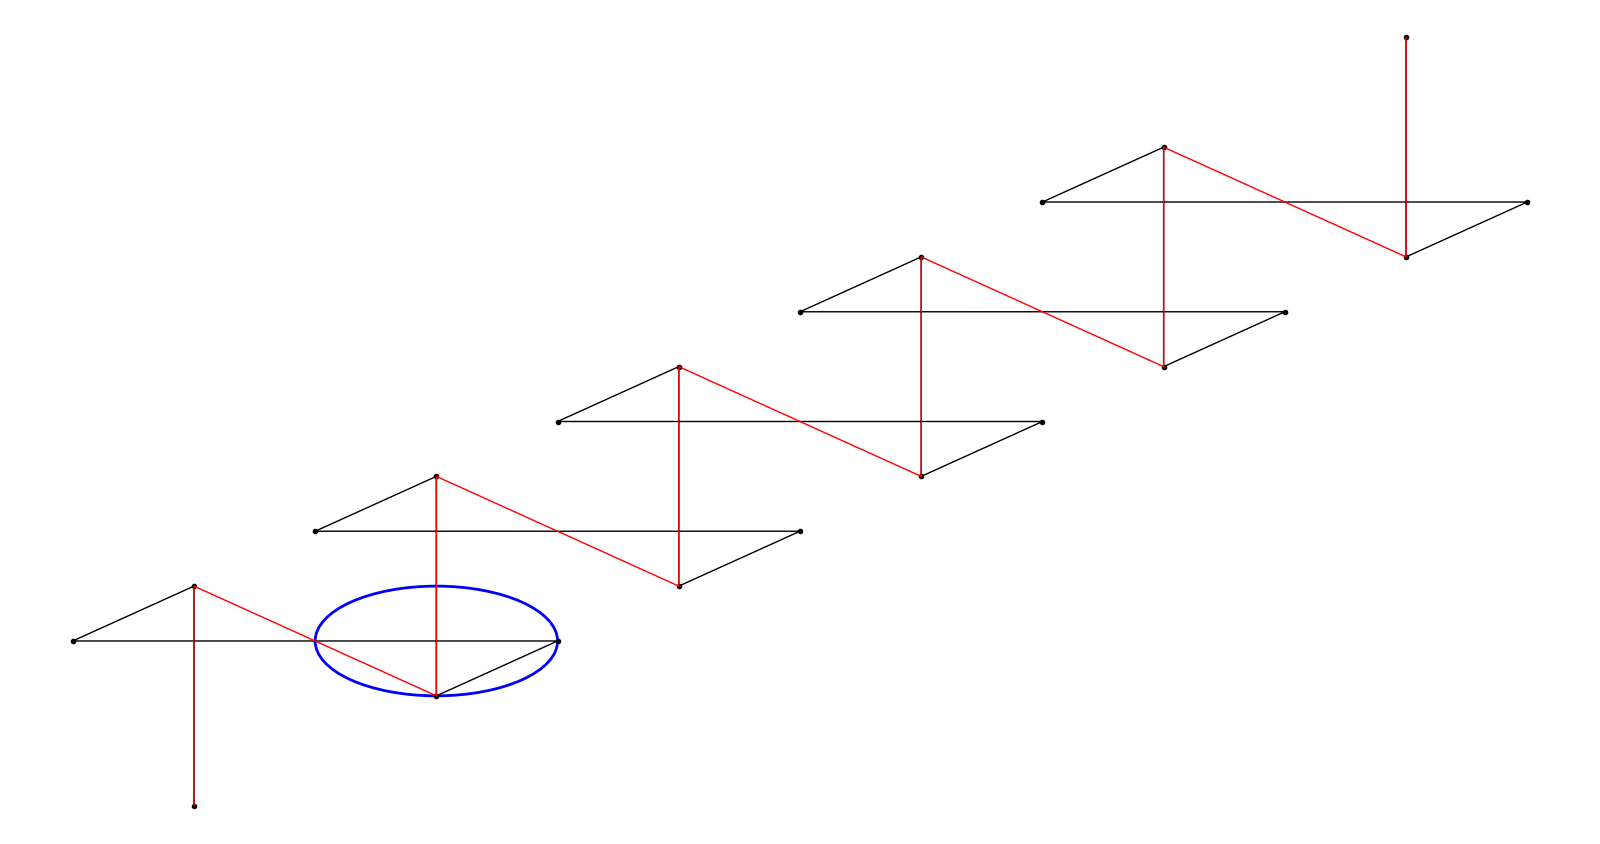
\includegraphics[scale=0.3]{./figures/local-global-bigdiff.png}
	\caption{Construction from \cref{thm:lg-approx} with \(i = 5\), a polyline consisting of multiple ``4"s. The local simplification contains all points and the global one is marked in red. The circle in blue has radius \(\varepsilon = 2\) and is centered around the self-intersection of the polyline.}
  \label{fig:local-global-bigdiff}
\end{figure}

This example demonstrates that local and global simplifications can differ by much but is not optimal. In fact, local simplifications can be arbitrarily bad in comparison to global ones.
\begin{theorem}
	Let \(n \in \N\) with \(n \geq 3\) and \(\varepsilon > 0\). There is a polyline with \(n\) vertices such that \(S(\delta^{LF}_2; P, \varepsilon) = n\) but \(S(\delta^F_2; P, \varepsilon) = 3\).

	It is impossible to achieve a greater difference in the simplification sizes.
\end{theorem}

\begin{proof}
  The only way how the difference could be bigger is if the global simplification uses only two vertices. This however would also be a local simplification and thus, the difference in sizes would actually be \(0\).

	For the actual construction see \cref{fig:local-global-mostdiff}. The idea is to choose an irrational angle \(\alpha\) in \((2\pi/4, 2\pi/3)\) like \(2\) radians. We consider the unit circle with radius \(\varepsilon\) and pick a point on it. Then we place the next point on the circle after rotation of \(\alpha\) and continue. We add a first point outside the circle such that \(\overline{P(0)P(1)}\) contains the center of the unit circle. The point count and angle are mostly arbitrary within the given bounds but should satisfy that \(\delta_2(P(1), P(n)) \leq \varepsilon\).

	For the global simplification only three points suffice: \(P(0)\), \(P(1)\) and \(P(n)\). The radius of the circle lies by construction on the first line segment of the simplification and is within distance of the whole polyline (except \(P(0)\)). Thus we can just proceed through the whole polyline while waiting at the center. After this we can finish the shortcut and as \(\delta_2(P(1),P(n)) \leq \varepsilon\) we can just append the shortcut to the last point.

	We now need to show that no local shortcuts exist. No shortcut other than \(\overline{P(0)P(1)}\) passes through the center as we rotate by an irrational angle. Any shortcut that contains the center must be constructed by two points that have a total angle of \(180^\circ\) between them which is rational but the sum of irrational angles is always irrational. This prevents us from skipping large parts of the polyline with a shortcut that contains the center like in the global case. The other possible shortcuts are easy to rule out because of the cyclical nature of the polyline. Shortcuts \(\overline{P(i-1)P(i+1)}\) that skip exactly one point \(P(i)\) cannot exist because by the choice of angle, no point on the shortcut is within \(\varepsilon\) of \(P(i)\). For any longer shortcut \(\overline{P(i')P(i)}\) we can similarly see that at least one of the skipped points has no point on the shortcut within distance \(\varepsilon\). Thus no local shortcuts exist and a local simplification requires all points.
\end{proof}

\begin{figure}[h!tbp]
  \centering
	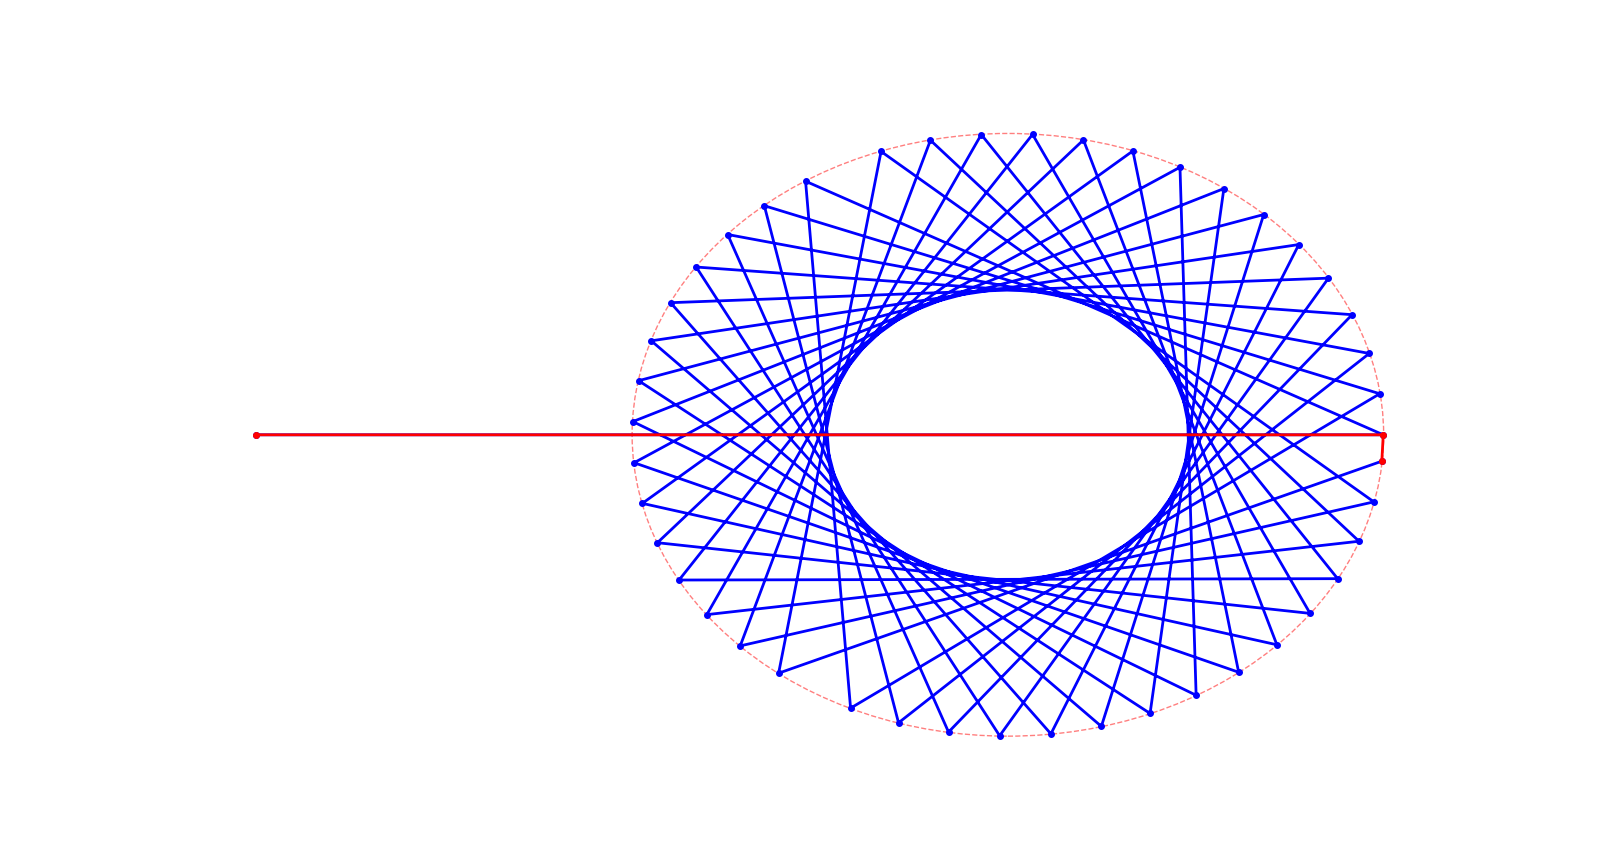
\includegraphics[scale=0.3]{./figures/local-global-mostdiff.png}
	\caption{Example polyline where the local and global sizes have maximal difference.}
  \label{fig:local-global-mostdiff}
\end{figure}

Unlike the previous example, this one uses mostly irrational coordinates. If one wants to test a simplification algorithm on such a polyline, we recommend placing the points not exactly on the circle but at a distance of \((1-\alpha)\varepsilon\) from the center where \(\alpha > 0\) is very small, otherwise, the global simplification might not be found. If the points are too close to the center the local simplification might be smaller. Fort this reason we have also provided the more stable previous example.

\subsection{A First Simplification Algorithm}
We conclude this section with a simple simplification algorithm for both the local and global Fréchet variants under any distance. This, however, only covers the case \(\varepsilon = 0\).

We know that \(\delta(u, v) = 0\) if and only if \(u = v\) for two points \(u\) and \(v\). A similar condition holds for polylines.

\begin{lemma}\label{lem:polyline_dist0}
	Let \(P\) and \(Q\) be polylines of length \(p\) and \(q\), respectively. Then \(\delta^F(P, Q) = 0\) if and only if there exists \(k \in \N\) with \(k \leq \min(p, q)\) and strictly increasing functions \(f:\set{0,\dots,k} \to \set{0,\dots,p}\) and \(g:\set{0,\dots,k} \to \set{0,\dots,q}\) with \(f(0) = g(0) = 0\), \(f(k) = p\), and \(g(k) = q\) such that:
	\begin{enumerate}
		\item \(P(f(t)) = Q(g(t))\) for all \(t \in \set{0, \dots, k}\).
		\item For each \(\ell \in \set{1, \dots, k}\) and each integer \(i\) with \(f(\ell-1) < i < f(\ell)\), there exists \(t_i \in [0,1]\) such that \(P(i) = (1-t_i)P(f(\ell-1)) + t_iP(f(\ell))\), and the sequence \(t_i\) is non-decreasing in \(i\).
		\item For each \(\ell \in \set{1, \dots, k}\) and each integer \(i\) with \(g(\ell-1) < i < g(\ell)\), there exists \(t_i \in [0,1]\) such that \(Q(i) = (1-t_i)Q(g(\ell-1)) + t_iQ(g(\ell))\), and the sequence \(t_i\) is non-decreasing in \(i\).
	\end{enumerate}
\end{lemma}

\begin{proof}
	(\(\Rightarrow\)) First, Assume \(\delta^F(P, Q) = 0\). Then there exist continuous, non-decreasing functions \(f'~:~[0,1]~\to~[0,p]\) and \(g':[0,1] \to [0,q]\) such that \(P(f'(t)) = Q(g'(t))\) for all \(t \in [0,1]\). \newline Let \(U = \set{u \mid u = P(i) = Q(j) \text{ for some } i=0,\dots,p, j=0,\dots,q}\). Define \(k = |U| - 1\), and let \(f\) and \(g\) map indices to the points in \(U\) in order. This satisfies Property (1).

	For Properties (2) and (3), the Fréchet condition ensures that between consecutive points in \(f\) (or \(g\)), the polyline must consist of a single line segment without bends, and the points on these segments must be in order. If there were multiple segments or out-of-order points, the Fréchet distance could not be zero.

	(\(\Leftarrow\)) If the conditions hold, the polylines are identical up to the addition of points on line segments. It is straightforward to construct functions \(f'\) and \(g'\) such that \(P(f'(t)) = Q(g'(t))\) for all \(t \in [0, 1]\).
\end{proof}

According to \cref{lem:polyline_dist0}, two polylines have Fréchet distance zero if and only if they differ only by points that lie on the line segments of the polyline. In other words, by removing all collinear points, the polylines become identical.

This leads to a linear-time algorithm for optimal simplification when \(\varepsilon = 0\). The start and end points must be included. For each intermediate point, we test if it lies on the line segment between its neighbors. If not, it is added to the simplification; otherwise, it is skipped.

\begin{algorithm}[ht]
  \DontPrintSemicolon
  \KwData{Polyline \(P\) of length \(n\)}
  \KwResult{Smallest \(0\)-simplification of \(P\)}
  \BlankLine
	\(simplification \gets [0]\)\;
	\For{\(i=1\) \KwTo \(n - 1\)}{
		\If{\(P(i)\) does not lie on \(\overline{P(i-1)P(i+1)}\)}{
			\(simplification.\text{append}(i)\)
		}
	}
	\(simplification.\text{append}(n)\)
	\Return{\(simplification\)}
  \caption{PolylineSimplificationWithEpsilon0(\(P\))}
  \label{algo:simplify_epsilon0}
\end{algorithm}

Testing if a point lies on a line segment is straightforward. For completeness, we derive the condition. A point \(p\) lies on \(\overline{uv}\) if and only if there exists \(t \in [0,1]\) such that \(p = u + t(v-u)\), or equivalently, \(p - u = t(v-u)\). Thus, for all coordinates \(i\), we need \(t = (p_i - u_i)/(v_i - u_i)\) to be the same. To avoid division by zero, we can reformulate this as \((p_{i-1} - u_{i-1})(v_i - u_i) = (p_i - u_i)(v_{i-1} - u_{i-1})\) for all \(i \geq 1\). To ensure \(t \in [0, 1]\), we require \(u_i \leq p_i \leq v_i\) (or \(v_i \leq p_i \leq u_i\)) for any coordinate where \(u_i \neq v_i\).


\section{Equation Solving}
\label{sec:equation_solving}
Before delving into the actual algorithms, we first need to address a problem at the core of the following procedures: the \emph{line segment intersection problem}. 
\begin{definition}[Line Segment Intersection Problem]
  Let \(e = \overline{e_1e_2}\) be a \(d\)-dimensional line segment, \(u \in \R^d\) a point, \(\varepsilon > 0\) and \(\delta\) a distance function. In the \emph{line segment intersection problem}, we aim to determine the set \newline \(\set{t \in [0, 1] \mid \delta(e_1 + t(e_2 - e_1), u) \leq \varepsilon}\), where \(t\) represents the parameter along the line segment \(e\).

  As the name suggests, this corresponds to the intersection of \(\set{x \in \R^d \mid \delta(x, u) \leq \varepsilon}\), the set of points within distance \(\varepsilon\) of \(u\), and the line segment \(e\). 
\end{definition}

\begin{observation}
  For \(\ell \in [1, \infty]\) the solution set to the line segment intersection problem using the distance \(\delta_\ell\) is convex. Thus we can express it as a single interval \(I \subseteq [0, 1]\). This interval is empty or closed, which allows us to identify it by its left and right boundaries. 
\end{observation}
\begin{proof}
  Follows directly from the convexity property of \cref{lem:distance_properties} and the fact that intervals and the points on line segments are convex sets. 
\end{proof}

This simplifies the process of finding these sets to determining the boundaries or identifying that the interval is empty. To do so, we solve equations involving distance functions \(\delta\). Specifically, we aim to solve 
\begin{equation}
  \delta(u + t \cdot (v - u), w) = \varepsilon \label{eq:eq_solve_main}
\end{equation}
for arbitrary, fixed vectors \(u, v, w \in \R^d\), and fixed \(\varepsilon \in \R_{>0}\), solving the variable \(t \in \R\), or determine that no such solution exists. This corresponds to the points that lie on the line \(e = \overline{uv}\) (not just the line segment) and have distance \(\varepsilon\) from \(w\).

We label the smallest solution of \cref{eq:eq_solve_main} \(\hat{t}_0\) and the largest solution \(\hat{t}_1\). Note that these may not be the solutions the line segment intersection problem as the solutions may be outside of the interval \([0, 1]\), i.e., they lie on the line defined by the two points but not the line segment. These two solutions may be the same (i.e, the interval collapses to a single point), or may not exist at all, in which case the interval is empty.

We need to modify the solutions \(\hat{t}_0\) and \(\hat{t}_1\) to obtain the actual solutions, \(\hat{t}_0'\) and \(\hat{t}_1'\), which can be defined as 
\begin{equation}
  \hat{t}_0' \coloneq \begin{cases}
    0 & \textrm{ if } \hat{t}_0 < 0 \textrm{ and } \hat{t}_1 \geq 0\\
    \hat{t}_0 & \textrm{ if } \hat{t}_0 \in [0, 1]\\
    \infty &\textrm{ otherwise }
  \end{cases}\\
  \hat{t}_1' \coloneq \begin{cases}
    1 & \textrm{ if } \hat{t}_1 > 1 \textrm{ and } \hat{t}_0 \leq 1\\
    \hat{t}_1 & \textrm{ if } \hat{t}_1 \in [0, 1]\\
    \infty &\textrm{ otherwise }
  \end{cases},
\end{equation}
where the \emph{otherwise} case also accounts for the absence of a solution to \cref{eq:eq_solve_main}. This corresponds to the smallest and largest points in the modified interval \([\hat t_0, \hat t_1] \cap [0, 1]\), which represents the actual solution to the line segment intersection problem. \cref{fig:solution_kinds} shows how this affects the solutions.
For a line segment \(\overline{uv}\) and a point \(w\) we denote \(\hat t_0'(\overline{uv}, w)\) and \(\hat t_1'(\overline{uv}, w)\) to be the respective modified solutions for the given line segment and point. We do not include \(\varepsilon\) in that notation as it is fixed throughout all algorithms and thus requires no disambiguation.

\begin{figure}
    \centering
    % First row of subfigures
    \begin{subfigure}[t]{0.3\textwidth}
      \includegraphics{tikz-fig/solution-kinds-1.pdf}
      \caption{\(\hat t_0 < 0 < \hat t_1 < 1\) \\ 
        \(\hat t_0' = 0, \hat t_1' = \hat t_1\)}
    \end{subfigure}
    \hfill
    \begin{subfigure}[t]{0.3\textwidth}
      \includegraphics{tikz-fig/solution-kinds-2.pdf}
      \caption{\(0 < \hat t_0 < \hat t_1 < 1\)\\ 
        \(\hat t_0' = \hat t_0, \hat t_1' = \hat t_1\)}
    \end{subfigure}
    \hfill
    \begin{subfigure}[t]{0.3\textwidth}
      \includegraphics{tikz-fig/solution-kinds-3.pdf}
      \caption{\(0 < \hat t_0 < 1 < \hat t_1 \) \\
        \(\hat t_0' = \hat t_0, \hat t_1' = 1\)}
    \end{subfigure}

    % Second row of subfigures
    \begin{subfigure}[t]{0.3\textwidth}
      \includegraphics{tikz-fig/solution-kinds-4.pdf}
      \caption{\(\hat t_0 < \hat t_1 < 0\)\\ 
        \(\hat t_0' = \hat t_1' = \infty\)}
    \end{subfigure}
    \hfill
    \begin{subfigure}[t]{0.3\textwidth}
      \includegraphics{tikz-fig/solution-kinds-5.pdf}
      \caption{\(\hat t_0 < 0 < 1 < \hat t_1\)\\ 
        \(\hat t_0' = 0, \hat t_1' = 1\)}
    \end{subfigure}
    \hfill
    \begin{subfigure}[t]{0.3\textwidth}
      \includegraphics{tikz-fig/solution-kinds-6.pdf}
      \caption{\(1 < \hat t_0 < \hat t_1\)\\ 
        \(\hat t_0' =  \hat t_1' = \infty\)}
    \end{subfigure}

    % Third row of subfigures (centered)
    \begin{subfigure}[t]{0.3\textwidth}
      \includegraphics{tikz-fig/solution-kinds-7.pdf}
      \caption{\(\hat t_0, \hat t_1\) do not exist\\ 
        \(\hat t_0' = \hat t_1' = \infty\)}
    \end{subfigure}
    \caption{The different kinds of solutions. Note that we associate \(0\) with \(u\), \(1\) with \(v\), and \(t\) with \((1-t)u + tv\)}
    \label{fig:solution_kinds}
\end{figure}

In general, determining these solutions requires finding roots of polynomials. Therefore, there is no exact solution algorithm for Minkowski distances \(\delta_e\) when \(e > 4\), as such polynomials are not solvable. Here, we derive explicit solutions for the Euclidean Distance, Manhattan Distance, and Chebyshev Distance. 

\subsection{Euclidean Distance}
\label{ssec:eq_euclidean_distance}
For the Euclidean distance, \cref{eq:eq_solve_main} simplifies to 
\begin{align*}
  \| (u - w) + t(v - u) \|_2 &= \varepsilon \\
  \| (u - w) + t(v - u) \|_2^2 &= \varepsilon^2 \\
  \| u - w \|_2^2 + 2\braket{u - w | v - u} t  +  \| v - u \|_2^2 t^2 &= \varepsilon^2 \\
  \underbrace{\delta(u,w)^2 - \varepsilon^2}_{\alpha_0} + 2\underbrace{\braket{u - w | v - u} }_{\alpha_1}t  +  \underbrace{\delta(v, u)^2}_{\alpha_2} t^2 &= 0 \\
  \alpha_0 + 2\alpha_1 t  + \alpha_2 t^2 &= 0.
\end{align*}

Here, we use Dirac notation for the inner product as \(\langle \cdot , \cdot \rangle\) denotes a polyline of length \(1\).
This is a quadratic equation in \(t\) and can be solved explicitly as 

\begin{equation}
	\hat t_{0,1} = \frac{-2\alpha_1 \pm \sqrt{(2\alpha_1)^2 - 4\alpha_0\alpha_2}}{2\alpha_2} = \frac{-\alpha_1 \pm \sqrt{\alpha_1^2 - \alpha_0\alpha_2}}{\alpha_2}.\label{eq:sol_explicit_euclidean}
\end{equation}

If the discriminant \(\alpha_1^2 - \alpha_0\alpha_2\) is negative, there is no real solution. Otherwise, we can compute the two roots and identify the smallest and largest among them. 


\subsection{Manhattan Distance}
\label{ssec:eq_manhattan_distance}
For the Manhattan distance, \cref{eq:eq_solve_main} simplifies to 
\begin{equation}
  \sum_{i=0}^d |u_i - w_i + t (v_i - u_i)| = \varepsilon. \label{eq:solve_manhattan}
\end{equation}

To handle both the Manhattan and Chebyshev distances, we make use the following observation: 
\begin{observation}\label{obs:permute-coordinates}
  Let \(u, v \in \R^d\) and let \(\sigma: \set{1, \dots, d} \to \set{1, \dots, d}\) be a permutation. Define \(\sigma(u) \in \R^d\) as the vector obtained by permuting the coordinates of \(u\) according to \(\sigma\), i.e., \(\sigma(u)_i = u_{\sigma(i)}\) for each \(i\). Then \(\delta_\ell(u, v) = \delta_\ell(\sigma(u), \sigma(v))\) for any \(\ell \in [1, \infty]\).
\end{observation}

Note that the term \(|u_i - w_i + t (v_i - u_i )|\) takes on either the value \(u_i - w_i + t(v_i - u_i)\) or its negation, depending on the sign. For a fixed \(t\), each term in the sum becomes a linear expression in \(t\), and the entire equation reduces to a linear equation, which is trivial to solve. 

We define 
  \[t_i \coloneq \frac{w_i - u_i}{v_i - u_i},\]
which is the zero of the respective coordinate. Let \(\sigma:\set{1,\dots, d} \to \set{1,\dots, d}\) be the sorting permutation such that 
  \[t_{\sigma(1)} < t_{\sigma(2)} < \cdots < t_{\sigma(d)}.\] 
By applying this permutation to both \(u-w\) and \(v -u\), the overall distance remains unchanged by \cref{obs:permute-coordinates}. 

Within any interval \(t \in [t_{\sigma(i)}, t_{\sigma(i+1)}]\), each term in the sum can be simplified to a linear form without absolute values. Thus, over each such interval, the equation can be solved analytically. We then verify whether the obtained solution lies within the current interval. 

A na\"ive implementation using a sweep-line approach would compute the \(t_i\), sort them, and evaluate each interval in linear time. To check each of the \(d+1\) intervals\footnote{Additionally, we need to account for the intervals \((-\infty, t_{\sigma(1)}]\) and \([t_{\sigma(d)}, \infty)\)} requires \(\O(d^2)\) runtime in total. However, by observing that only a single term in the sum changes sign between adjacent intervals, we can incrementally update the linear expression in constant time, reducing the complexity to \(\O(d \log d)\), dominated by the sorting step. 

We also address two edge cases:
\begin{itemize}
	\item Coinciding \(t_i\): No special treatment is needed; these form single point intervals and thus can be ignored. If the solution is exactly the point in that interval it is also in the neighboring intervals as the total function is continuous in \(t\).
	\item \(u_i = v_i\): In this case, the corresponding term becomes a constant and can be subtracted from \(\varepsilon\).
\end{itemize}

\begin{algorithm}[ht]
  \DontPrintSemicolon
  \KwData{vectors \(u, v, w \in \R^d\), \(\varepsilon > 0\)}
  \KwResult{Solution to \cref{eq:solve_manhattan}}
  \BlankLine
  \(global\_slope \gets 0, global\_offset \gets 0\) \;
  \(events \gets Array(d)\)
  \For{\(i = 1, \dots, d\)}{
    \(slope \gets v_i - u_i, offset \gets u_i - w_i\)\;
    \If{\(slope < 0\)}{
      \(slope \gets -slope, offset \gets -offset\)
    } \ElseIf{\(slope = 0\)}{
      \(\varepsilon \gets \varepsilon - |offset|\)\;
      \Continue
    }
    \(zero \gets - \frac{offset}{slope}\)\;
    \If{\(zero \leq 0\)}{
      \(global\_offset \gets global\_offset + offset\)\;
      \(global\_slope \gets global\_slope + slope\)\;
      \Continue
    } 
    \(global\_offset \gets global\_offset - offset\)\;
    \(global\_slope \gets global\_slope - slope\)\;
    \If{\(zero \geq 1\)}{
      \Continue
    }
    \(events.append((zero, slope, offset))\)\;
  }
  Sort \(events\) by their \(zero\) component\;
  \(start \gets 0\)\;
  \For{\((zero, slope, offset) \in events\)}{
    Test if solution \(\frac{\varepsilon - global\_offset}{global\_slope} \in [start, zero]\) and report it if so\;
    \(global\_offset \gets global\_offset + 2offset\)\;
    \(global\_slope \gets global\_slope + 2slope\)\;
    \(start \gets zero\)
  }
  Test if solution \(\frac{\varepsilon - global\_offset}{global\_slope} \in [start, 1]\) and report it if so\;

  \caption{manhattan\_solver(\(u, v, w, \varepsilon\))}
  \label{algo:solve_manhattan}
\end{algorithm}

Finally, we can further reduce the runtime to expected linear time by observing that a full ordering of the \(t_i\) values is unnecessary. Instead, we only require the two values that bound the potential solutions. This allows us to use a modified version of the Quickselect algorithm to find the relevant boundaries in \(\O(d)\) expected time\footnote{This holds under the assumption of random pivot selection. A deterministic worst-case linear runtime is also achievable using robust pivot strategies, such as the median-of-medians method.}. 

The structure of the algorithm remains similar. We work with an array of candidate pairs \((a, b)\), each representing a term of the form \(|a+bt|\). Initially, we define artificial left and right boundary tuples \((1, 0)\) and \((-1, 0)\), representing infinite bounds\footnote{We can also use the artificial bounds \((0, 1)\) to represent \(0\) and \((-1, 1)\) to represent \(1\) and ignore all coordinates outside of the interval \((0, 1)\) as previously. Note again that the zero of \((a, b)\) is \(-\frac{a}{b}\) forcing a negative sign.}. 

To compare tuples \((a, b)\) and \( (c,d)\), we define an ordering based on the location of their respective zero crossing, i.e.,
  \[(a, b) < (c, d) \quad \iff \quad -\frac{a}{b} < - \frac{c}{d} \quad \iff \quad ad > bc.\]
This comparison is division-free, compatible with the artificial boundaries, and ensures numerical stability.  

At each iteration, we 
\begin{enumerate}
	\item Choose a pivot \((a, b)\)	and find all tuples in the array that have the same zero (i.e., the same \(-\frac{a}{b}\)).
	\item Merge those terms into the pivot by adding their components, keeping the same zero-crossing.
	\item Partition the array into those before and after the pivot (based on the ordering defined above).
	\item Maintain the global linear equation not only for the start but also directly before the pivot, updating it as in \cref{algo:solve_manhattan}.
\end{enumerate}

We then evaluate the distance at the pivot point using the current linear expression. Since the Manhattan distance is a convex function of \(t\), we can determine which direction to search based on the slope: 
\begin{itemize}
	\item If the distance at the pivot is greater than \(\varepsilon\), we can continue in the direction that the slope at the pivot indicates\footnote{If the slope at the pivot is negative, the solution must lie to the right. If the slope is positive, the solution lies to the left.}.
	\item If the distance at the pivot is less than \(\varepsilon\), then one solution lies to the left of the pivot and one to the right. We can then search each side independently to find both.
\end{itemize}

This approach behaves like a simplified convex-aware gradient descent and ensures that solutions are found (if they exist) with high efficiency. 

 It is also possible that no solution exists, in which case the function value at all breakpoints will exceed \(\varepsilon\). 

 Throughout the search, we update the left and right boundary tuples to maintain the current interval of interest, replacing either with the pivot depending on which half of the array we are searching. 

\subsection{Chebyshev Distance}
\label{ssec:eq_chebyshev_distance}
For the Chebyshev distance, \cref{eq:eq_solve_main} simplifies to 
\begin{equation}
  \max_{i = 1,\dots, d} |u_i - w_i + t(v_i - u_i)| = \varepsilon.\label{eq:solve_chebyshev}
\end{equation}

\paragraph{Na\"ive Approach.}
A simple algorithm evaluates all possible breakpoint candidates. Each absolute value expression \(|u_i - w_i + t(v_i - u_i)|\) has two branches (positive and negative), resulting in \(2d\) candidate expressions. At each such candidate value \(t\), we compute whether that term is indeed the global maximum in \cref{eq:solve_chebyshev}. This leads to a straightforward \(\O(d^2)\) time algorithm: each candidate is evaluated in \(\O(d)\) time.

For low dimensions, especially \(d = 2\), this approach is practical. Furthermore, as with the Manhattan case, we may restrict considerations to \(t \in [0, 1]\), reducing the number of candidates.

\paragraph{Geometric Approach. }
To improve performance, we observe that each term in the maximum of \cref{eq:solve_chebyshev} is linear in \(t\), forming a collection of \(2d\) linear functions. Solving this equations corresponds to tracking the upper envelope of these lines over the interval \([0, 1]\) and identifying when the envelope reaches value \(\varepsilon\).

We can adapt a sweep-line method inspired by the Bentley-Ottmann algorithm~\cite{computational_geometry}, modified for our use case: 
\begin{enumerate}
	\item We sort all lines in decreasing order of their initial value (offset), breaking ties using slope.
	\item We construct a doubly linked list to maintain the ordering of active lines. When two lines intersect, the lower one is removed, and only the upper continues to be tracked.
	\item A priority queue holds upcoming intersections. At each step, we remove the lower line at the intersection and enque the next relevant intersection. 
	\item When the topmost line changes, we check whether it intersects the level \(\varepsilon\) between the last and current intersection.
\end{enumerate}

This process guarantees that only \(\O(d)\) relevant intersections are processed, even if there are potentially \(\O(d^2)\) total line intersections. A self-balancing tree is unnecessary as deletion is the only operation that needs to be performed dynamically. An array-based doubly-linked list suffices, where each element stores previous and next nodes and the line parameters which are the offset and slope. 

Pseudocode for this approach is provided in \cref{algo:solve_chebyshev_init} and \cref{algo:solve_chebyshev}. An example run of this algorithm is illustrated in \cref{fig:chebyshev_algo}. For a complete solution, the logic from \cref{sec:equation_solving} on tracking valid solutions must also be applied.

\begin{figure}
  \centering 
  \begin{subfigure}[t]{0.3\textwidth}
		\includegraphics{tikz-fig/chebyshev-algo-1.pdf}
    \caption{All candidate lines}
  \end{subfigure}
  \begin{subfigure}[t]{0.3\textwidth}
    \includegraphics{tikz-fig/chebyshev-algo-2.pdf}
    \caption{Lines that are not fully negative}
  \end{subfigure}
  \begin{subfigure}[t]{0.3\textwidth}
    \includegraphics{tikz-fig/chebyshev-algo-3.pdf}
    \caption{Lines that are not fully below another line}
  \end{subfigure}\\
  \begin{subfigure}[t]{0.3\textwidth}
    \includegraphics{tikz-fig/chebyshev-algo-4.pdf}
    \caption{Find next intersection. Here between topmost line so check for solution.}
  \end{subfigure}
  \begin{subfigure}[t]{0.3\textwidth}
    \includegraphics{tikz-fig/chebyshev-algo-5.pdf}
    \caption{Find next intersection. No solution found}
  \end{subfigure}
  \begin{subfigure}[t]{0.3\textwidth}
    \includegraphics{tikz-fig/chebyshev-algo-6.pdf}
    \caption{Check final line for an intersection}
  \end{subfigure}
  \caption{Line representation of the equation \(\delta_\infty((0,0,0) + t(-2,0,3), (-2,-1,1)) = 1.5\)}
  \label{fig:chebyshev_algo}
\end{figure}

\begin{algorithm}[ht]
  \DontPrintSemicolon
  \KwData{vectors \(u, v, w \in \R^d\), \(\varepsilon > 0\)}
  \BlankLine
  \(candidates \gets \set{(2i, u_i - w_i, v_i - u_i), (2i+1, w_i - u_i, u_i - v_i) | i = 0, \dots, d - 1}\) \;
  \(queue \gets PriorityQueue()\) \;
  \(list \gets Array(|candidates|)\) \;
  sort candidates according to second component descendingly,
  in case of ties use the third component as tie breaker descendingly \;
  \(PREV \gets 0, NEXT \gets 1\) \tcp{constants for readability}
  \(curr \gets -1\) \;
  \For{\((i, a, b) \in candidates\)}{
    \If{\(curr = -1\)} {
      \(curr \gets i, a' \gets a, b' \gets b\)\;
      \(list[curr] \gets (-1, -1, a, b)\) \;
      \Continue
    } 

    \If{\( a' + b' \geq a + b\)}{
      \Continue \tcp{new line fully below current line so never maximum}
    } 

    \(list[curr][NEXT] \gets i, list[i] \gets (curr, -1, a, b)\) \;
    \(intersection \gets \frac{a' - a}{b - b'}\) \tcp{always in \([0,1]\)}
    \(queue.insert\_with\_priority((curr, i), intersection)\) \;
    \(curr \gets i, a' \gets a, b' \gets b\) \;
  }

  \caption{chebyshev\_solver\_initialization(\(u, v, w\))}
  \label{algo:solve_chebyshev_init}
\end{algorithm}

\begin{algorithm}[ht]
  \DontPrintSemicolon
  \KwData{vectors \(u, v, w \in \R^d\), \(\varepsilon > 0\)}
  \KwResult{Solution to \cref{eq:solve_chebyshev}}
  \BlankLine
  \(chebyshev\_solver\_initialization(u, v, w)\) \;
  \(last\_intersection \gets 0\) \;
  \While{\(\lnot queue.empty()\)}{
    \((i, j), intersection \gets queue.poll()\) \;
    \If{\(list[i][PREV] = -1 \lor list[j][PREV] = -1\)}{
      \Continue \tcp{One of the lines already removed, no intersection}
    } 
    \If{\(i = HEAD\)}{
      \(HEAD \gets j\) \;
      \(\_, \_, a, b \gets list[i]\) \;
      \If{\(b = 0\)}{
        \If{\(a = \varepsilon\) }{
          Mark \(last\_intersection\) as earliest solution or \(intersection\) as last solution \;
        }
        \(last\_intersection \gets intersection\) \;
        \Continue 
      }
      \(solution \gets \frac{\varepsilon - a}{b}\) \;
      Mark \(solution\) as earliest or last solution if \(solution \in [last\_intersection, intersection]\) \;
      \(last\_intersection \gets intersection\) \;
      \Continue
    }
    \(before_i \gets list[i][PREV]\) \;
    \(list[before_i][NEXT] \gets j, list[j][PREV] \gets before_i\) \;
    \(list[i][PREV] \gets -1\) \tcp{mark as removed}
    \(last\_intersection \gets intersection\) \;
    \If{\(before_i \neq HEAD\)}{
      \(\_, \_, a, b \gets list[j]\) \;
      \(\_, \_, a', b' \gets list[before_i]\) \;
      \(intersection \gets \frac{a' - a}{b - b'}\) \tcp{also in \([0,1]\)}
      \(queue.insert\_with\_priority((before_i, j), intersection)\) \;
    }
  }
  Check for solution in \([last\_intersection, 1]\) \;

  \caption{chebyshev\_solver(\(u, v, w, \varepsilon\))}
  \label{algo:solve_chebyshev}
\end{algorithm}

\paragraph{Algebraic Approach.}
There exists a simpler, linear-time algorithm to solve \cref{eq:solve_chebyshev}, based on rewriting the condition as a system of inequalities.

\begin{observation}
	Let \(a_1, \dots, a_d, b_1, \dots, b_d, t \in \R\). Then
	\[\max_{i=1,\dots, d} |a_i + tb_i| = \varepsilon \iff \forall i \in \set{1,\dots, d}:  |a_i + tb_i| \leq \varepsilon \land \exists i \in \set{1,\dots, d}: |a_i + tb_i| = \varepsilon.\]
\end{observation}

This observation allows us to reduce the problem to computing and intersecting a set of intervals. Each inequality \(|a_i + tb_i| \leq \varepsilon\) defines a valid interval for \(t\), given by 
	\[t \in \left[\frac{-\varepsilon - a_i}{b_i}, \frac{\varepsilon - a_i}{b_i}\right] \quad \text{if } b_i > 0.\]

If \(b_i < 0\), we can flip the sign of both \(a_i\) and \(b_i\) to make the slope positive. If \(b_i = 0\), the term reduces to \(|a_i|\). This yields
\begin{itemize}
	\item No solution if \(|a_i| > \varepsilon\),
	\item A trivially satisfied constraint if \(|a_i| < \varepsilon\) that can be ignored, or 
	\item An always-satisfied constraint if \(|a_i| = \varepsilon\) that must be accounted for as a possible solution.
\end{itemize}

The solution set is the intersection of all valid intervals, which can be computed in linear time by maintaining the maximum of the left interval boundaries and the minimum of the right ones. We then verify whether any expression \(|a_i + tb_i| = \varepsilon\) is realized within this interval.

\paragraph{Summary}
We have described three methods to solve \cref{eq:solve_chebyshev}: A na\"ive, quadratic runtime method, an efficient, geometric \(\O(d\log d)\) method and a simple and elegant \(\O(d)\) method using interval intersection. For practical implementations, the linear method is typically preferable due to its clarity and performance.





\section{Algorithm \& Implementation}
\label{sec:algorithm_implementation}

In this section we will sketch \citeauthor{on_optimal_polyline_simplification_using_the_hausdorff_and_frechet_distance}'s algorithm for polyline simplification as well as a simplified version of \citeauthor{computing_the_frechet_distance_between_two_polygonal_curves}'s algorithm to decide if two polylines have Fréchet distance of at most \(\varepsilon\). We will see an example of these algorithms and end with optimizations that can be applied.

\subsection{Fréchet Distance Decision Algorithm}
\label{ssec:alt_godau}
The simplification algorithm we will describe heavily uses a subroutine to solve the following problem: Given \(\varepsilon > 0\), a polyline \(P\) of length \(p\), a subpolyline \(P[j' + t' \dots j+1]\), and a line segment \(\overline{P(i')P(i)}\) (where \(i' < i \leq p, j' \leq j < p\in \N\), and \(t' \in [0, 1]\)), decide whether there exists \(t \in [0, 1]\) such that \(\delta^F(P[j' + t' \dots j + t], \overline{P(i')P(i)}) \leq \varepsilon\). If so, return the smallest such \(t\).  

This can be solved by a simplified version of \citeauthor{computing_the_frechet_distance_between_two_polygonal_curves}'s algorithm to decide if the Fréchet distance of two polylines is at most \(\varepsilon\). We present the algorithm in the specific form needed for this problem. 

By definition, the Fréchet distance requires the starting points to match, i.e., \(\delta(P(j' + t'), P(i')) \leq \varepsilon\). If this fails, we immediately return ``no solution". We set \(t_0 \coloneq \hat t_0'(\overline{P(j)P(j+1)}, P(i))\) and \(t_1 \coloneq \hat t_1'(\overline{P(j)P(j+1)}, P(i))\). Similarly, as the end points must match, we get that \(t \in [t_0, t_1]\). Thus if there is no such interval we can return that there is no solution.

We distinguish the two cases \(j' = j\) and \(j' < j\). 
\begin{enumerate}
	\item[\(j' = j\): ] The subpolyline reduces to a single line segment \(\overline{P(j)P(j+1)}\). The constraints simplify to \(t \in [t', 1] \cap [t_0, t_1]\), which is feasible if and only if \(t' \leq t_1\). The solution is then \(\max(t', t_0)\).

	\item[\(j' < j\): ] We iterate over the intermediate points \(P(k) = P(j'+1), \dots, P(j)\) and compute the solutions \(\hat t_0'(\overline{P(i')P(i)}, P(k))\), and \(\hat t_0'(\overline{P(i')P(i)}, P(k))\). We maintain the first reachable point \(s\) on the line segment \(\overline{P(i')P(i)}\) (initially \(s = 0\)) for these points and test if \(s \leq \hat t_1'(\overline{P(i')P(i)}, P(k))\). If this fails we return that there is no solution. Otherwise we update \(s = \max(s, \hat t_0'(\overline{P(i')P(i)}, P(k)))\). Finally, we have fully traversed the line segment and most of the subpolyline. At this point the solution is merely \(t_0\).
\end{enumerate}

The correctness for the first case follows directly from \cref{lem:distance_properties}. The correctness of case \(j' < j\) can also be shown relatively easily. 

\begin{lemma}\label{lem:ag-neq}
	Let \(P = \angl{u_0, \dots, u_p}\) be a polyline of length \(p\) and \(e = \overline{v_0v_1}\) be a line segment. Then 
	\(\delta^F(P, e) \leq \varepsilon\) if and only if 
	\begin{enumerate}
		\item \(\delta(u_0, v_0) \leq \varepsilon\),
		\item \(\delta(u_p, v_1) \leq \varepsilon\), and
		\item There are \(x_i \in [\hat t_0'(e, u_i), \hat t_1'(e, u_i)]\) for \(i \in \set{1, \dots, p - 1}\) with \(x_1 \leq \cdots \leq x_{p-1}\).
	\end{enumerate}
\end{lemma}
\begin{proof}
	For the forward direction there are function \(f \in \mathcal{C}([0,1], [0, p])\) and \(g \in \mathcal{C}([0,1], [0, 1])\) with \(\delta(P(f(t)), e(g(t))) \leq varepsilon\) for all \(t \in [0, 1]\). By plugging in \(0\) or \(1\) we get the first two properties. For the third one pick \(x' \in [0, 1]\) such that \(f(x) = i\) and pick \(x_i = g(x)\). Such an \(x\) exists as \(f\) is continuous (but it may not be unique). Then \(\delta(P(i), e(x_i)) \leq \varepsilon \) implying that \(x_i \in [\hat t_0'(e, u_i), \hat t_1'(e, u_i)]\). Furthermore, \(x_1 \leq \cdots \leq x_{p-1}\) as \(1 < \cdots < p-1\) and both \(f\) and \(g\) are monotonous.

	For the backward direction, we must construct suitable function \(f\) and \(g\). For \(g\) we pick the identity and we define \(f(x_i) = i\) for all \(i \in \set{1, \dots, p - 1}\) and additionally \(f(0) = 0\) and \(f(1) = p\). All other points are linearly interpolated between the defined points resulting in \(f((1-t)x_i + tx_{i+1}) = i + t\) for \(t\in [0,1]\) (where we extend \(x_0 = 0\) and \(x_p = 1\)). The correctness of \(f\) follows directly from the convexity property from \cref{lem:distance_properties} as well as \(x_1 \leq \cdots \leq x_{p-1}\) which guarantees monotonicity.
\end{proof}

\subsection{Polyline Simplification Algorithm}
\label{ssec:simple_algo_main}

Here we outline the global polyline simplification algorithm from \citeauthor{on_optimal_polyline_simplification_using_the_hausdorff_and_frechet_distance} which we have implemented and tested for the Euclidean distance, the Manhattan distance, and the Chebyshev distance. 

Similar to the decision problem we use a dynamic program in which we store the earliest reachable points although in a more complicated manner. We build a 3D table \(DP[k,i,j] \in [0, 1] \cup \set{\infty}\) for each triple \((k, i, j)\) with \(k, i \in \set{0, \dots, n}\) and \(j \in \set{0, \dots, n - 1}\) where \(n\) is the length of the given polyline \(P\). 

Each entry \(DP[k, i, j]\) stores the smallest \(t \in [0, 1]\) s.t. there is a simplification \(Q\) of \(P[0 \dots i]\) with exactly \(k\) line segments with \(\delta^F(Q, P[0\dots j + t]) \leq \varepsilon\). If no such \(t\) exists we store \(\infty\) in that entry. 
To retrieve the simplification from this table, we find the smallest \(k^*\) s.t. \(DP[k^*, n, n - 1]\) exists, i.e., there is a simplification \(Q\) of the whole polyline with \(k^*\) many line segments that has \(\delta^F(Q, P[0\dots n - 1 + t]) \leq \varepsilon\) for some \(t \in [0, 1]\) so we can complete the simplification by simply going from \(n-1+t\) to \(n\) on the last line segment of \(P\) while staying on the last point of the simplification. 

For \(k = 0\) it is trivial to compute the entries. If \(i > 0\) no simplification exists, i.e., we can store \(\infty\), as it is impossible to create a simplification of size \(0\) that goes to any point other than the initial point. To find \(DP[0, 0, j]\) we only need to compute the distances from \(P(0)\) to the points \(P(j)\) (see \cref{fig:simpl_init}). Until the first \(j\) with \(\delta(P(0), P(j)) > \varepsilon\) we can store \(0\). From the first such \(j\) we store \(\infty\). Since the simplification consists only of a single point \(P(0)\), the condition \(\delta^F(Q, P[0\dots j + t]) \leq \varepsilon\) simplifies to \(\delta^F(P[0 \dots 0], P[0 \dots j + t])\) and as we cannot move on the single point \(P(0)\) the earliest reachable point on each line segment must be \(t = 0\). 

The correctness of this initialization can be shown rather easily. 
\begin{lemma}
  Let \(P = \angl{P(0)}\) a polyline consisting of a single point and \(Q\) be a polyline of size \(n\). Then \(\delta^F(P, Q) \leq \varepsilon\) if and only if \(\delta(P(0), Q(i)) \leq \varepsilon\) for all \(i \in \set{0, \dots, n}\). 
\end{lemma}
\begin{proof}
  For the forward direction, there exist functions \(f\) and \(g\) such that \(\delta(P(f(t)), Q(g(t))) \leq \varepsilon\) for all \(t\in [0,1]\), where \(f(0) = g(0) = 0\), \(f(1) = 0\), \(g(1) = n\), and \(f\) and \(g\) are  monotone. This implies that \(\delta(P(0), Q(g(t))) \leq \varepsilon\). As \(g\) is continuous and \(g(0) = 0 \leq g(1) = n\) there must be some \(t \in [0,1]\) with \(g(t) = x\) for any \(x\in \set{0, \dots, n}\).
  
  For the backward direction, we show that every point on \(Q\) has distance at most \(\varepsilon\) from \(P(0)\) thus we can choose any suitable function \(g\) (for \(f:[0,0] \to [0,0]\) there is only one possibility). This follows directly from the convexity property from \cref{lem:distance_properties} applied to all individual line segment on \(Q\).
\end{proof}

\begin{figure}[b]
  \centering
  \includegraphics{tikz-fig/simpl_init.pdf}
  \caption{Initialization of the simplification algorithm for \(k = 0, i = 0\). Only the points in the circle until \(P(2)\) are reachable.}
  \label{fig:simpl_init}
\end{figure}


As for the other entries, the authors show that the entry \(DP[k, i, j]\) can be computed by the minimization over all \(i' < i\) and \(j' \leq j\). We lookup the value \(t' \coloneq DP[k-1, i', j']\) and test if there is a \(t \in [0, 1]\) to which we can proceed, i.e., \(\delta^F(P[j' + t' \dots j + t], \overline{P(i')P(i)}) \leq \varepsilon\) and return the smallest such \(t\) if possible. This can be done with the algorithm from \citeauthor{computing_the_frechet_distance_between_two_polygonal_curves} with the mentioned modifications. Among all those candidates \(t\) we choose the minimal one. If no such \(t\) exists we can store \(\infty\).

\begin{algorithm}[ht]
  \DontPrintSemicolon
  \KwData{Polyline \(P\) of length \(n\), \(\varepsilon > 0\)}
  \KwResult{Smallest \(\varepsilon\)-simplification of \(P\)}
  \BlankLine
  \(DP \gets Array((n + 1, n + 1, n))\) initialized with \(\infty\) \;
  \For{\(j = 0, \dots, n\)}{
    \If{\(\delta(P(0), P(j)) > \varepsilon\)}{
      \Break
    }
    \(DP[0, 0, j] \gets 0\)
  }
  \For{\(k=1,\dots\) until \(DP[k, n, n-1] \neq \infty\)}{
    \For{\(i=0,\dots, n\)}{
      \For{\(j=0,\dots, n-1\)}{
        \For{\(i' < i\)}{
          \For{\(j' \leq j\)}{
            Let \(t' \gets DP[k-1, i', j']\)\;
						\If{\(t' = \infty \)}{
							\Continue
						}
            Let \(t \gets AltGodau(P[j' + t' \dots j + 1], \overline{P(i')P(i)}, \varepsilon)\)\;
            \(DP[k, i, j] \gets \min(DP[k, i, j], t)\)
          }
        }
      }
    }
  }
  \caption{PolylineSimplification(\(P, \varepsilon\))}
  \label{algo:simplify_simple}
\end{algorithm}

There are \(\O(k^* n^2)\) many iterations to fill in the table and each entry requires \(\O(n^2)\) many computations to find the minimum where \(k^*\) is the size of the output simplification. Each call to the \(AltGodau\) subroutine requires linear runtime thus in total we have \(\O(k^*n^5)\) run time.

\subsection{Examples}
Before discussing possible optimizations, we want to go through an example for the algorithm as well as the \citeauthor{computing_the_frechet_distance_between_two_polygonal_curves} subroutine. This gives us more intuition for the algorithms as well as ideas for further optimizations. Because of the cubic number of entries it is unreasonable to show all computations thus we only show the computations that lead to the simplification and the subroutine for them. 

\begin{figure}
  \centering
  \includegraphics{tikz-fig/poly-ex-main.pdf}
  \caption{Example polyline with circles with radius \(\varepsilon\) drawn around all points. We note the following relations which may be hard to notice: \(\delta(P(2), P(4)) = \delta(P(2), P(5)) = \varepsilon\), \(\delta(P(2), P(3)) > \varepsilon\), \(\delta(P(2), P(6)) > \varepsilon\).}
  \label{fig:poly-ex-main}
\end{figure}

For the polyline and \(\varepsilon\) in \cref{fig:poly-ex-main} we initialize the table layer for \(k = 0\) by only setting the value \(DP[0,0,0]\) to \(0\) as \(\delta(P(0), P(1)) > \varepsilon\). Even though \(\delta(P(0), P(4)) \leq \varepsilon\) the value \(DP[0,0,4]\) is \(\infty\) as there are points between that already fail.

For the layer \(k = 1\) we can only proceed from the entry \(DP[0,0,0] = 0\) as it is the only one we found on the previous layer. All triples \(k, i, j\) for which a valid entry in \([0, 1]\) can be found for the layer \(k = 1\) are listed in \cref{tab:exlayer1}. We do not list the respective \(i', j'\) and \(t'\) as there is only one possible entry.
\begin{table}[ht]
\centering
\begin{tabular}{|ccc|}
\hline
$(1,1,0)$ & $(1,1,1)$ & $(1,1,2)$ \\
$(1,2,0)$ & $(1,2,1)$ & $(1,2,2)$ \\
$(1,2,3)$ & $(1,2,4)$ & $(1,2,5)$ \\
$(1,3,2)$ & $(1,3,3)$ & $(1,4,0)$ \\
$(1,4,1)$ & $(1,4,2)$ & $(1,5,0)$ \\
$(1,5,1)$ & $(1,5,2)$ & \\
\hline
\end{tabular}
\caption{Valid entries for layer \(k = 1\). All proceed from \((0,0,0)\).}
\label{tab:exlayer1}
\end{table}

Let us explicitly go through the AltGodau subroutine for the entry \((1, 2, 3)\), i.e., A simplification consisting of one line segment for the subpolyline \(P[0\dots 2]\) that has distance of at most \(\varepsilon\) from \(P[j' + t'\dots j + t] = P[0 \dots 3 + t]\) where \(t\) is gotten from the subroutine. We consider the line segment \(\overline{P(i')P(i)} = \overline{P(0)P(2)}\) and the polyline segment \(P[j' + t' \dots j + 1] = P[0 \dots 4]\) and perform the algorithm. 

\begin{figure}
  \centering
  \begin{subfigure}[b]{0.4\textwidth}
    \includegraphics{tikz-fig/poly-ex-123-ag-1.pdf}
  \end{subfigure}
  \begin{subfigure}[b]{0.4\textwidth}
    \includegraphics{tikz-fig/poly-ex-123-ag-2.pdf}
  \end{subfigure}\\
  \begin{subfigure}[b]{0.4\textwidth}
    \includegraphics{tikz-fig/poly-ex-123-ag-3.pdf}
  \end{subfigure}
  \begin{subfigure}[b]{0.4\textwidth}
    \includegraphics{tikz-fig/poly-ex-123-ag-4.pdf}
  \end{subfigure}
  \caption{Finding the first reachable point on \(\overline{P(3)P(4)}\). Resulting in \(t = 0.04\) marginally below point \(P(3)\). Note again that \(\delta(P(2), P(3)) > \varepsilon\). The point \(P(4)\) is not part of the simplification, it only lies on the line segment \(\overline{P(0)P(2)}\) by chance.}
  \label{fig:poly-ex-123-ag}
\end{figure}

From \(DP[1,2,3] = 0.04\) we can proceed to the end of the polyline to get a simplification of size \(2\) as seen in \cref{fig:poly-ex-265-ag}. A simplification of size \(1\) is not possible as that would be the line segment \(\overline{P(0)P(6)}\) but there is no point on that line segment within distance \(\varepsilon\) from \(P(3)\). 

\begin{figure}
  \centering
  \begin{subfigure}[b]{0.4\textwidth}
    \includegraphics{tikz-fig/poly-ex-265-ag-1.pdf}
  \end{subfigure}
  \begin{subfigure}[b]{0.4\textwidth}
    \includegraphics{tikz-fig/poly-ex-265-ag-2.pdf}
  \end{subfigure}\\
  \begin{subfigure}[b]{0.4\textwidth}
    \includegraphics{tikz-fig/poly-ex-265-ag-3.pdf}
  \end{subfigure}
  \caption{Finding the first reachable point on \(\overline{P(5)P(6)}\). With that we have found a simplification for the whole polyline.}
  \label{fig:poly-ex-265-ag}
\end{figure}

We can also convince ourselves that the solution must be correct as the application of the algorithm from \citeauthor{computing_the_frechet_distance_between_two_polygonal_curves} guarantees that the Fréchet distance is at most \(\varepsilon\) by construction and even yields the points that can be used to construct suitable functions that show this. 

For completeness sake the entries on the layer \(k = 2\) are listed in \cref{tab:exlayer2}. The entry \((k - 1, i', j')\) they reference from the previous layer is added after the tuple. This predecessor tuple is not necessarily unique, in fact, every single one of these has at least two different possibilities for \(i', j'\).
\begin{table}[ht]
\centering
\begin{tabular}{|ccc|}
\hline
$(2,4,3):(2, 1)$ & $(2,4,4):(2, 1)$ & $(2,5,4):(2,4)$ \\
$(2,5,5):(2,4)$ & $(2,6,5):(2,4)$ & \\
\hline
\end{tabular}
	\caption{Valid entries for layer \(k = 2\). Each entry proceeds from \((1, i', j')\) where \(i'\) and \(j'\) are annotated as a tuple after the colon.}
\label{tab:exlayer2}
\end{table}

In total, for all three layers there were only \(1 + 17 + 5 = 23\) entries, far smaller than \(7^4 = 2401\), the (approximate) number of iterations iterations over all \(i, j, i', j'\). This motivates ideas to reduce the runtime.

\subsection{Optimizations}
\label{ssec:optimizations}
Based on the just described algorithm we outline optimizations that greatly reduce the \(\O(k^*n^5)\) runtime in practice. The most effective optimizations circumvent the theoretical runtime by skipping iterations. 

We first note that for the entry \((k, i, j)\) in the dynamic program we do not always need to iterate over all possible \(i' < i\) and \(j' \leq j\). As we are interested in the minimal value \(t\) on the line segment \(\overline{v_{j}v_{j+1}}\) that can be reached, we can stop further search if we have reached a lower bound for that value. Such a lower bound is \(\hat t_0'(\overline{v_{j}v_{j+1}}, i)\), i.e. the modified solution to the \cref{eq:eq_solve_main}, which is tight as for a sufficiently large \(k\) this value must be reached eventually. This allows an early break out of the search through the \(i' < i, j'\leq j\) and a speed up of upto quadratic runtime. This is the \emph{local minimality} optimization. 

Another optimization based on a similar insight is the following: If the entry at \((k-1, i, j) = \hat t_0'(\overline{v_{j}v_{j+1}}, i)\), i.e., we have found a simplification for the same \(i\) and \(j\) that has already reached the optimal value, we know this cannot be improved in the current layer \(k\) or any further one. This means, the entry at \((k, i, j)\) can never be used by some entry \((k + 1, i'', j'')\) because of minimality as any such entry that uses \((k, i, j)\) could have already used \((k-1, i, j)\) for \((k, i'', j'')\). This enables us to completely ignore the computation of the value, resulting in a continuous speed up of the algorithm while it runs as once this happens for an entry, it will happen for all further ones with a higher value of \(k\) so with each layer more entry computations can be skipped. This is the \emph{global minimality} optimization.

Another way to skip computations is to ignore all \(i\) with \(i < k\) as well as all \(i'\) with \(i' < k - 1\) in the computations as there can never be a simplification of \(P[0\dots i]\) that uses more than \(i\) line segments thus it must always hold that \(i \geq k\). This optimization does not get a name and all our implementations have this inherently.

A last simple optimization of a similar type which is particularly useful for well-behaved polylines is to not even start the iterations over the \(i', j'\) if there is no solution \(\hat t_0'(\overline{v_{j}v_{j+1}}, i)\). This happens often if there are not too many line segments close to each other. This is the \emph{reachability} optimization. 





\section{Implicit Polyline Simplification}\label{sec:implicit_polyline_simplification} 
In this section, we review the polyline simplification algorithm and all of its dependencies in order to avoid explicitly computing the solutions of distance equations. We abstract the instances which need explicit solutions to these equations in \citeauthor{on_optimal_polyline_simplification_using_the_hausdorff_and_frechet_distance}'s algorithm for polyline simplification and the required Fréchet distance decision algorithm from \citeauthor{computing_the_frechet_distance_between_two_polygonal_curves} to a small set of decision problems. 
We show how these decision problems can be solved for the Euclidean distance without square roots or even divisions, meaning, only addition, subtraction, and multiplication are required. Correctness for the implicit algorithms follows directly from the correctness of the explicit version as only the comparison is abstracted while the actual logic is unaffected. 

\subsection{Decision Problems}
We introduce three decision problems, each based on a relation. 
\begin{definition}[Implicit Decision Relations]\label{def:implicit_relations}
  Let \(e = \overline{e_1e_2}\) be a line segment, and \(u, v\) with \(e_1, e_2, u\) and \(v\) having the same dimension. 
  \begin{itemize}
    \item We say \(u\) \emph{reaches} \(e\) (in symbols \(u \leftrightarrow e\)) if there is a point \(x\) on \(e\) with \(\delta(u,x)\leq \varepsilon\). This is equivalent to the existence of \(\hat t_0'(e, u)\).
    \item Let \(u \leftrightarrow e\). We say \(u\) \emph{proceeds to} \(v\) \emph{in} \(e\) (in symbols \(u \overset{e}\rightarrow v\)) if, and only if 
      \begin{itemize}
        \item \(v \leftrightarrow e\), 
        \item \(\hat t_0'(e, u) \leq \hat t_0'(e, v)\)
      \end{itemize}

    \item Let \(u \leftrightarrow e\). We say \(u\) \emph{waits for} \(v\) \emph{on} \(e\) (in symbols \(u \overset{e}\leftarrow v\)) if, and only if
      \begin{itemize}
        \item \(v \leftrightarrow e\), 
        \item \(\hat t_0'(e, v) \leq \hat t_0'(e, u) \leq \hat t_1'(e, v)\)
      \end{itemize}
  \end{itemize}
  For \(u \overset e\rightarrow v\), we say that \(v\) becomes the new \emph{restriction point} and similarly if \(u \overset e\leftarrow v\) we say that \(u\) remains the restriction point.
\end{definition}

As a note, for \(e = \overline{e_1e_2}\) and a point \(u\) it holds \(u \leftrightarrow e\) if, and only if, \(e_1 \overset{e}\rightarrow u\). Thus it is not necessary to provide an implementation for \(\leftrightarrow\) directly. We separate the relations because \(\rightarrow\) is more complex but often the simpler \(\leftrightarrow\) relation suffices and is geometrically more intuitive.

We will see how we can implement the previous algorithms using procedures to decide these relations for a line segment and points. The idea is, instead of computing the solutions to the required equations and then comparing them throughout the algorithms, we have procedures to compare them directly. This allows us to only maintain the point that causes the solution of the equation, which we call the restriction point as it restricts the earliest reachable point on a line segment. A visual example of these relations can be seen in \cref{fig:restrictions}.

A trivial fact we will use to find initial restrictions is that \(u \overset e\rightarrow v\) always holds if \(v \leftrightarrow e\) and \(u\) is the starting point of \(e\). Also, if both \(u \overset e\rightarrow v\) and \(u \overset e\leftarrow v\) then the first solutions of both are the same, i.e., \(\hat t_0'(e, u) = \hat t_0'(e,v)\), thus either is a restriction. 

\begin{figure}[ht]
  \centering
  \begin{subfigure}[t]{0.3\textwidth}
    \includegraphics[width=\linewidth]{tikz-fig/restrictions-1.pdf}
    \caption{\(u \overset e\rightarrow v\). We go from \(\hat t_0'(e, u)\) to \(\hat t_0'(e, v)\) and \(v\) becomes the new restriction point.}
  \end{subfigure}
  \begin{subfigure}[t]{0.3\textwidth}
    \includegraphics[width=\linewidth]{tikz-fig/restrictions-2.pdf}
    \caption{Neither \(u \overset e\rightarrow v\) nor \(u \overset e\leftarrow v\).}
  \end{subfigure}
  \begin{subfigure}[t]{0.3\textwidth}
    \includegraphics[width=\linewidth]{tikz-fig/restrictions-3.pdf}
    \caption{\(u \overset e\leftarrow v\). We cannot go backward but \(v\) is reachable so we can wait for it and \(u\) remains the restriction point. }
  \end{subfigure}
  \caption{Illustration of the relations and how to interpret them. }
  \label{fig:restrictions}
\end{figure}

\subsection{Fréchet Distance Decision}
We review the algorithm from \citeauthor{computing_the_frechet_distance_between_two_polygonal_curves} and adapt it to use the relations from \cref{def:implicit_relations} instead of solving equations. This can be done both for the general problem of deciding for two polylines if their Fréchet distance is at most \(\varepsilon\) as well as for the modified version we are interested in which returns the earliest reachable point on the last line segment\footnote{Obviously, this requires modifications to the statement of the algorithm as we cannot explicitly compute the solution. These modifications will be mentioned later.}. 

For the general Fréchet distance decision problem fix two given polylines \(P\) of length \(p\) and \(Q\) of length \(q\) with a fixed \(\varepsilon > 0\) and \(p \geq q\) (otherwise swap the two polylines). We decide if \(\delta^F(P, Q) \leq \varepsilon\) by using the dynamic programming approach from \citeauthor{computing_the_frechet_distance_between_two_polygonal_curves}. 

We start by explaining only the version needed where \(q = 1\), meaning the second polyline is a single line segment. As we cannot return an explicit solution to the equation we return the restriction point \(r\) on the last line segment that causes the solution instead. Furthermore, the input also takes an initial restriction point \(r'\) for the line segment \(\overline{P(0)P(1)}\) so that we do not have to compute the initial point of the subpolyline. 

The start of the algorithm is similar, we first need to test if the initial points match and if so we can distinguish the two cases where \(p = 1\) or \(p > 1\). To test if the initial points match is equivalent to testing \(r \overset e\leftarrow Q(0)\) for \(e = \overline{P(0)P(1)}\) as the initial point on \(P\) is \(P(\hat t_0'(e, r))\) so the initial points of the polylines have a distance of at most \(\varepsilon\) if this point is in the interval \([\hat t_0'(e, Q(0)), \hat t_1'(e, Q(0))]\).

\begin{itemize}
  \item[Case \(p = 1\): ] Set \(e = \overline{Q(0)Q(1)}\). The first points of the two line segments already match so we only need to fully traverse \(Q\). We either need to proceed on \(P\) from the restriction or wait, so the result is \(r\) if \(r \overset e\leftarrow Q(1)\) and \(Q(1)\) if \(r \overset e\rightarrow Q(1)\). If neither case occurs there is no solution. 
    See \cref{fig:alt_godau_implicit_eq} for visual examples of this.
  \item[Case \(p > 1\): ] We first traverse the line segment \(e = \overline{Q(0)Q(1)}\) and maintain the current restriction \(r'\) which is initially \(r\). We iterate through \(P(1), P(2), \dots, P(p-1)\) and for each point \(P(i)\) we test if \(r' \overset e\rightarrow P(i)\). If so we update \(r'\) to \(P(i)\). If \(r' \overset e\leftarrow P(i)\) there is no need to update \(r'\). If neither occurs there is no solution. 

    Finally, \(P[0\dots p-1]\) is traversed and we need to determine the restriction on the line \(e'=\overline{P(p-1)P(p)}\). As the only possible restriction on this line segment we get \(Q(1)\) as we only need to fully traverse \(e\). If \(Q(1) \leftrightarrow e'\) we can return \(Q(1)\) otherwise there is no solution.
\end{itemize}

\begin{figure}
    \centering
    \begin{subfigure}[t]{0.3\textwidth}
      \includegraphics[width=\linewidth]{tikz-fig/alt-godau-implicit-eq-1.pdf}
      \caption{\(r \overset e\leftarrow Q(0)\) and \(r \overset e\rightarrow Q(1)\) for \(e = \overline{P(0)P(1)}\). We proceed from the restriction \(r\) to the new restriction \(Q(1).\)}
    \end{subfigure}
    \begin{subfigure}[t]{0.3\textwidth}
      \includegraphics[width=\linewidth]{tikz-fig/alt-godau-implicit-eq-2.pdf}
      \caption{\(r \overset e\rightarrow Q(1)\) but not \(r \overset e\leftarrow Q(0)\) for \(e = \overline{P(0)P(1)}\). Invalid way to proceed on the line.}
    \end{subfigure}
    \begin{subfigure}[t]{0.3\textwidth}
      \includegraphics[width=\linewidth]{tikz-fig/alt-godau-implicit-eq-3.pdf}
      \caption{\(r \overset e\leftarrow Q(0)\) and \(r \overset e\leftarrow Q(1)\) so we can proceed on \(\overline{Q(0)Q(1)}\) while remaining on the same restriction point \(r\) on \(e = \overline{P(0)P(1)}\)}
    \end{subfigure}

    \caption{Modified implicit Fréchet distance, case \(p = 1\).}
    \label{fig:alt_godau_implicit_eq}
\end{figure}

The general algorithm can be adapted with the same ideas, replacing the first reachable points with the respective restrictions in the dynamic program. 

\subsection{Simplification Algorithm}
Now that we have already modified the Fréchet distance decision algorithm for the implicit case, adapting the Simplification algorithm from \citeauthor{on_optimal_polyline_simplification_using_the_hausdorff_and_frechet_distance} is relatively simple. 

The dynamic programming table \(DP\) stores point indices from \(\set{0, \dots, n}\) or a value that indicates that there is no solution for that entry, e.g., \(\infty\). the point index stored at \(DP[k,i,j]\) is the restriction point \(r\) on the line segment \(\overline{P(j)P(j+1)}\) that would create the solution in the explicit case. 

The initialization remains the same with a slight abuse of data types. The \(0\) that indicates the first reachable point on the line segment for the explicit approach now indicates that the point \(P(0)\) is the restriction point. This results in the same solution as we only store \(0\) for points that have distance within \(\varepsilon\) from \(P(0)\). Thus the first solution on any line segment that starts with such a point must be \(0\) which is the same as in the explicit approach.

For \(k > 0\) we only need to adapt how we use the Fréchet distance decision subroutine. During the iteration over \(i\), \(j\), \(i' < i\) and \(j' \leq j\), the explicit approach would retrieve the earliest reachable point \(DP[k-1, i', j']\) which marks the start of the subpolyline that we consider. Then it would compute the earliest reachable point on the line segment \(\overline{P(j)P(j+1)}\) and return this as a solution. Both such points will be replaced with the respective restriction point that bound them. We have already shown how to adapt the algorithm to take as input the restriction point from \(DP[k-1,i',j']\) and returns the new one on the line segment so it only remains to show how to minimize this point. 

Throughout the inner iterations over \(i'\) and \(j'\) we maintain the restriction on the line segment \(e = \overline{P(j)P(j+1)}\) that causes the first reachable point. This is initially \(\infty\) and when we find the first actual point we just store it. Once we have a current minimum restriction \(r\) and a new candidate \(r'\) we need to determine whose solution comes first on \(e\). For this we only need to test \(r \overset e\to r'\). If so, \(r\) remains and otherwise \(r'\) becomes the new current minimum. Note that here the left side of \(\to\) remains the restriction instead of the right side becoming the new one as we minimize the restriction.

This already concludes the necessary modifications to the algorithm. As a final note, we mention how to apply the optimizations to this approach. The reachability optimization is equivalent to testing \(P(i) \leftrightarrow \overline{P(j)P(j+1)}\). For the minimality conditions we only need to determine the restriction point that causes the boundary we compared against. A brief lookup shows that we only need to compare the restriction against \(i\) in both cases. \cref{algo:simplify_simple_implicit} shows the full algorithm with the optimizations.

\begin{algorithm}[ht]
  \DontPrintSemicolon
  \KwData{Polyline \(P\) of length \(n\), \(\varepsilon > 0\)}
  \KwResult{Smallest \(\varepsilon\)-simplification of \(P\)}
  \BlankLine
  \(DP \gets Array((n + 1, n + 1, n))\) initialized with \(\infty\) \;
  \For{\(j = 0, \dots, n\)}{
		\If{\(\delta'(P(0), P(j)) > \nu(\varepsilon)\)}{
      \Break
    }
    \(DP[0, 0, j] \gets 0\)
  }
  \For{\(k=1,\dots\) until \(DP[k, n, n-1] \neq \infty\)}{
    \For{\(i=k,\dots, n\)}{
      \For{\(j=0,\dots, n-1\)}{
				\If{\(DP[k-1,i,j] = i\)} {
					\(DP[k,i,j] \gets i\)\;
					\Continue \tcp{Global Minimality}
				}
				\If{\(\lnot P(i) \leftrightarrow \overline{P(j)P(j+1)}\)} {
					\Continue \tcp{Reachability}
				}
        \For{\(k - 1 \leq i' < i\)}{
          \For{\(j' \leq j\)}{
            Let \(r' \gets DP[k-1, i', j']\)\;
						\If{\(r' = \infty\)}{
							\Continue 
						}
            Let \(r \gets AltGodau(P[j' \dots j + 1], r', \overline{P(i')P(i)}, \varepsilon)\)\;
						\If{\(r \neq \infty \land P(r) \overset e\to P(r')\)} {
							\(DP[k, i, j] \gets r\)\;
							\If{\(r = i\)} {
								Skip further iterations over \(i', j'\) \tcp{Local Minimality}
							}
						}
          }
        }
      }
    }
  }
  \caption{PolylineSimplification(\(P, \varepsilon\))}
  \label{algo:simplify_simple_implicit}
\end{algorithm}


\subsection{Euclidean Implementation}
Having seen how we can use these decision problems to implement the algorithms, we make use of them in the Euclidean case. By avoiding the explicit computation of solutions of \cref{eq:eq_solve_main} we can avoid computing square roots and even avoid divisions leading us to the following results. 

\begin{theorem}
  For \(d\)-dimensional polylines \(P\) and \(Q\) of length \(p\) and \(q\) respectively, it is possible to decide if \(\delta_2^F(P, Q) \leq \varepsilon\) in runtime \(\O(d p q)\) with the only arithmetical operations necessary being addition, subtraction and multiplication. 
\end{theorem}

\begin{theorem}\label{thm:euclidean_implicit_simplification_simple}
  For a \(d\)-dimensional polyline \(P\) of length \(n\) the problem of global polyline simplification using the Euclidean Fréchet distance can be solved in \(\O(d k^*n^5)\) with the only arithmetical operations necessary being addition, subtraction and multiplication where \(k^*\) is the size of the simplification.
\end{theorem}

As we expect that the adaptions from \citeauthor{polyline_simplification_has_cubic_complexity_bringmannetal} are compatible with our decision problems, the runtime of \cref{thm:euclidean_implicit_simplification_simple} can likely be adjusted to \(\O(d n^3)\). We will review, and hopefully verify, this in a following thesis. 
This theorem also extends to the Manhattan and Chebyshev distance (even with the cubic runtime algorithm) by using explicit computations but storing the results as a numerator-denominator pair. For this, note that we only compare the fractions but do not perform any computations with these thus the magnitudes of numerator and denominator do not explode.

The decision problems for the relations \(\leftrightarrow, \leftarrow\) and \(\rightarrow\) are simple to implement without division and square roots but quite technical. We start with \(\leftrightarrow\) which can be implemented as a special case of \(\rightarrow\) but can be solved even simpler. Fix a line segment \(e = \overline{e_1e_2}\) and a point \(u\). \(u \leftrightarrow e\) holds if, and only if, the distance to the closest point on \(e\) to \(u\) has distance at most \(\varepsilon\). This closest point with respect to the Euclidean distance is the projection of \(u\) onto \(e\). We write it as \(e_1 + t(e_2 - e_1)\) then \(t = \frac{\braket{e_2 - e_1 | u - e_1}}{\delta_2'(e_1, e_2)}\)~\cite{linear_algebra}. 

To decide \(u \leftrightarrow e\) we only need to test if either of the two end points is reachable from \(u\), i.e., \(\delta_2'(e_i, u) \leq \varepsilon^2\) for \(i = 1\) or \(i = 2\). If both fail we must check the projection. Thus we return true if, and only if, \(t \in [0, 1]\) and the following inequality is true. 

\begin{alignat*}{3}
&\delta_2'(e_1 + t(e_2 - e_1), u) &&\leq \varepsilon^2 \\
  \iff& \|e_1 - u + t(e_2 - e_1)\|^2 &&\leq \varepsilon^2 \\
  \iff& \delta_2'(e_1, u) + 2\braket{e_1 - u | e_2 - e_1}t + \delta_2'(e_1, e_2)t^2 &&\leq \varepsilon^2 \\
  \iff& \delta_2'(e_1, u) + 2\braket{e_1 - u | e_2 - e_1}\frac{\braket{e_2 - e_1 | u - e_1}}{\delta_2'(e_1, e_2)} + \delta_2'(e_1, e_2)\parenth{\frac{\braket{e_2 - e_1 | u - e_1}}{\delta_2'(e_1, e_2)}} &&\leq \varepsilon^2 \\
  \iff& \delta_2'(e_1, u)\delta_2'(e_1, e_2) - 2\braket{e_1 - u | e_2 - e_1}^2 + \braket{e_2 - e_1 | u - e_1}^2 &&\leq \varepsilon^2 \delta_2'(e_1, e_2)\\
  \iff& \delta_2'(e_1, u)\delta_2'(e_1, e_2) - \braket{e_1 - u | e_2 - e_1}^2 &&\leq \varepsilon^2 \delta_2'(e_1, e_2)
\end{alignat*}

For the other two relations we get very similar procedures. For simplicity we only derive \(u \overset e\rightarrow v\). We define \(a_{0u} \coloneq \delta_2'(e_1, u)\), \(a_{0v} \coloneq \delta_2'(e_1, v)\), \(a_{1u} \coloneq 2\braket{e_2 - e_1 | e_1 - u}\), \(a_{1v} \coloneq 2\braket{e_2 - e_1 | e_1 - v}\), and \(a_{2} \coloneq \delta_2'(e_1, e_2)\) which are the coefficients of the quadratic equation needed to solve for \(\hat t_{0/1}(e, u)\) and \(\hat t_{0/1}(e, v)\). We further denote the discriminants of the solutions \(D_u \coloneq a_{1u}^2 - 4a_{0u}a_2\) and \(D_v \coloneq a_{1v}^2 - 4a_{0v}a_2\). We define \(x  \coloneq a_{1u} - a_{1v}\) and \(y \coloneq D_u + D_v - x^2\). With these we get 

\begin{alignat*}{2}
  u \overset e\rightarrow v \iff& v \leftrightarrow e \land \hat t_0'(e, u) \leq \hat t_0'(e, u) \\
  \iff& v \leftrightarrow e \land \frac{-a_{1u} - \sqrt{D_u}}{2a_2} \leq \frac{-a_{1v} - \sqrt{D_v}}{2a_2} \\
  \iff& v \leftrightarrow e \land -a_{1u} - \sqrt{D_u} \leq -a_{1v} - \sqrt{D_v} \\
  \iff& v \leftrightarrow e \land -a_{1u} - \sqrt{D_u} \leq -a_{1v} - \sqrt{D_v} \\
  \iff& v \leftrightarrow e \land \sqrt{D_v} - \sqrt{D_u} \leq a_{1u} - a_{1v}  \\
  \iff& v \leftrightarrow e \land \sqrt{D_v} - \sqrt{D_u} \leq x  \\
  \iff& v \leftrightarrow e \land ((x \geq 0 \land \sqrt{D_v} \leq \sqrt{D_u})\\ & \lor (x \geq 0 \land \sqrt{D_v} \geq \sqrt{D_u} \land \sqrt{D_v} - \sqrt{D_u} \leq x )\lor(x \leq 0 \land \sqrt{D_v} \leq \sqrt{D_u} \land \sqrt{D_u} - \sqrt{D_v} \geq -x ) )  \\
  \iff& v \leftrightarrow e \land ((x \geq 0 \land D_v \leq D_u)\\ & \lor (x \geq 0 \land D_v \geq D_u \land \sqrt{D_v} - \sqrt{D_u} \leq x )\lor(x \leq 0 \land D_v \leq D_u \land \sqrt{D_u} - \sqrt{D_v} \geq -x ) ).
\end{alignat*}

Now we consider only the inequalities \(\sqrt{D_v} - \sqrt{D_u} \leq x\) and \(\sqrt{D_u} - \sqrt{D_v} \geq -x\) where we know that all sides of the inequalities are positive thus squaring them preserves the inequalities. We get 

\begin{align*}
  \sqrt{D_v} - \sqrt{D_u} \leq x &\iff D_v + D_u - 2\sqrt{D_uD_v} \leq x^2 \\
   &\iff y \leq 2\sqrt{D_uD_v} \\
   &\iff (y \leq 0) \lor (y^2 \leq 4D_uD_v)
\end{align*}

and similarly for the other inequality. With that this problem can be decided without square roots or divisions albeit in a rather technical manner.

\subsection{General Minkowski Distances}
Having seen how implicit computations simplifies simplification in the Euclidean case, we want to try to extend this technique to other Minkowski distances. As of writing this we do not know whether it is possible to implement all three decision problems without the use of approximations but implicit computations allows a simpler and possibly more numerically stable way to approximate. 

First, we consider the relation \(\leftrightarrow\). Again, we can easily check if \(\delta_\ell'(e_1, u) \leq \nu_\ell(\varepsilon)\) and \(\delta_\ell'(e_2, u) \leq \nu_\ell(\varepsilon)\) when testing \(u \leftrightarrow e\). If neither occurs we need to test \(\hat t_0'(e, u) \in [0,1]\). This can be solved using Sturm's theorem~\cite{algorithms_in_real_algebraic_geometry}. 
\begin{theorem}[Sturm's Theorem]
  Let \(p\) be a polynomial and \(p'\) be its derivative. The number of roots of \(p\) in the interval \((a,b)\) is 
  \[Var(p_0(a), p_1(a), \dots, p_k(a)) - Var(p_0(b), p_1(b), \dots, p_k(b)),\]
  where \(p_0 \coloneq p\), \(p_1 \coloneq p'\) and \(p_i \coloneq -Rem(p_{i-2}, p_{i-1})\) for \(i \in \set{2, \dots, k}\) until \(p_{k+1} = 0\). 
  Here \(Rem\) denote the remainder of the polynomial division and \(Var\) is the number of sign changes of a sequence, i.e., \(Var(a_0,\dots, a_k) = |\set{i \in \set{1, \dots, k} \mid a_ia_{i-1} < 0}|\).
\end{theorem}

In fact, as the interval is \((0, 1)\) this simplifies the computations as we only need to lookup the constant term and the sum of the coefficients for each polynomial. 
Multiplicities of roots does not affect the results as we are only interested in the existence of a root in the interval. 
The only necessary operations needed to implement this are addition, subtraction, multiplication, and division and as the degree of the polynomials is fixed for a given distance function we can estimate the required space for a sufficiently precise representation of the coefficients that occur during the polynomial division. 

As for the other two relations, it may be possible to use methods from real algebraic geometry to argue about the position of the roots of the polynomials. 

As a final note on the Minkowski distances we want to note that the absolute values for odd \(\ell\) can be dealt with similarly as with the Manhattan distance by sorting the inner linear terms according to their zero and partitioning the real numbers into intervals for which all absolute values can be simplified. There are at most two intervals in which the root of the polynomial can lie in and those can be found by evaluating the polynomials at the interval bounds. If any interval has a positive and negative bound there must be exactly one zero in that interval by the intermediate value theorem. Otherwise all interval bounds are positive. If there are solutions they must be in the interval with the smallest bounds. This leaves \(\O(d\log d)\) preprocessing to determine a constant amount of candidate intervals and thus a constant amount of polynomials to test. Alternatively, the linear runtime approach from the Manhattan distance can also be adapted to find the appropriate interval. 

\subsection{Semiexplit Decisions}
As a final point of our discussion of implicit simplification we present a method that uses aspects from both explicit computations and implicit decisions which we call semiexplicit. 

The idea is to implement the implicit decisions with an estimation of the roots. To test if \(u \overset e\rightarrow v\) we use a bisection approach. we test for both \(u\) and \(v\) if they have distance at most \(\varepsilon\) from any of the end points of \(e\). If \(\delta(u, e_1) \leq \varepsilon\) we can say that \(u \overset e\rightarrow v\). Otherwise if \(\delta(v, e_1) \leq \varepsilon\) this is false (but \(v \overset e\rightarrow u\) would be true). Otherwise suppose they both have solutions on the line segment. 

We performe the following for both \(x \in \set{u, v}\). We start with the following values \(a = 0, b = 1, t = 0.5\) and iterate  until \(d_t \coloneq \delta(e_1 + t(e_2 - e_1), x) \leq \varepsilon\). 
First, we test if \(d_t \leq \varepsilon\) and if we are done with this step. Otherwise we test if \(d_a \leq d_t \leq d_b\) in which case we proceed with \(b \gets t\) and \(t \gets \frac{a + t}2\). If \(d_a \geq d_t \geq d_b\) we proceed with \(a \gets t\) and \(t \gets \frac{b + t}2\). Otherwise it must be \(d_a \geq d_t \leq d_a\) as \(d_a \leq d_t \geq d_a\) is impossible due to property 3 of \cref{lem:distance_properties}.
We compute \(i \coloneq \frac{a + t}2\) and \(j \coloneq \frac{t + b}2\). It holds \(a < i < t < j < b\) and there are three different cases for the computed distances. If \(d_a \geq d_i \leq d_t\) we update \(b \gets t\) and \(t \gets i\). If \(d_t \geq d_j \leq d_b\) we update \(b \gets t\) and \(t \gets i\) and otherwise it holds \(d_i \geq d_t \leq d_j\) and we update \(a \gets i\) and \(b \gets j\). By doing this we improve a bound for the interval that contains the solutions and after this step we have found a point \(t\) that separates the two solutions. 

At this point we know the first solutions is in the interval \((a, t]\) we have computed for both. If the two intervals have an empty intersection we can directly answer which first solutions comes first. Otherwise we trim both intervals to their intersection and perform another bisection on this interval but compare both \(u\) and \(v\) simultaneously until we find a point that separates the first solution of both distances. This results in the solution. There are a few edge cases that need to be considered as well as the case that there is no solution in the interval for one of the points. We could use Sturm's theorem to test for solutions but this would likely be slower than using the bisection method until some threshold is reached.

The semiexplicit approach seems like a worse version of both the explicit approach as we need to perform multiple comparisons in the worst case, as well as a worse version of the implicit appraoch as we still rely on approximating solutions instead of comparing them directly. However, it has the advantage that it is the most general of the three approaches in the sense that it requires the least amount of primitives. The explicit approach requires both a distance function and an equation solver for that distance function. The implicit approach requires the distance function and at least solvers for the decision problems \(\leftarrow\) and \(\rightarrow\) and possibly even \(\leftrightarrow\). The semiexplicit only requires the distance function as a black box with no further information of it thus it also works for general\footnote{The distance function still must be convex in the sense of of \cref{lem:distance_properties}} distance functions on \(\R^d\), not only Minkowski distances. Furthermore, the approximations can speed up computations if the first solutions for both points can be separated easily. In the worst case the solutions are close or even coincide which results in many iterations, this however is rather unlikely and may not even affect the overall solution to the simplification at all\footnote{Of course, it is possible to construct a degenerate polyline where the solutions are arbitrarily close and the result matters.}.

It can also be optimized by storing the resulting intervals into the dynamic programming table as a substitute for the earliest reachable point in the explicit approach. The respective restriction point is still required just like in the implicit approach because the interval may need to be improved when comparing agains another one. This allows fewer computations in total while still keeping the advantage of lazy computations with which we mean that the solution is only approximated to a precision that is sufficient allowing fast decisions for sufficiently well behaved polylines.

\subsection{Open Problems}
To conclude this discussion on implicit polyline simplification we want to list some questions, mostly of theoretical nature. 

The first and simplest, but also broadest, question is to which current algorithms this approach extends. We have shown that it works for the algorithm from \citeauthor{computing_the_frechet_distance_between_two_polygonal_curves} as well as the algorithm from \citeauthor{on_optimal_polyline_simplification_using_the_hausdorff_and_frechet_distance}. We suspect that it also extends to the algorithm from \citeauthor{polyline_simplification_has_cubic_complexity_bringmannetal} and will investigate this in a future thesis. For other algorithms, especially for local polyline simplification there are no results. We are optimistic that it extends to most other current, as well as future algorithms, albeit possibly by introducing more decision problems. This process of reanalyzing the algorithms is tedious but technically simple. 

Another open question is whether the decision problems can be fully answered for general \(\ell\)-Minkowski distances with \(\ell \in \N\). We have already proposed a method to decide the \(\leftrightarrow\) relation using simple methods from real algebraic geometry but failed to solve the other two relations. This requires a more sophisticated approach and will likely involve more properties of the distance polynomials, e.g., that they have at most two roots, or that they are the sum of linear terms to the power \(\ell\). These results will likely be only of theoretical interest as they simplify the required computational model but do not lead to practical algorithms. 



\section{Simplification Algorithm from Bringmann and Chaudhury}
\label{sec:cubic_algo}
In this section, we explain the algorithm from \citeauthor{polyline_simplification_has_cubic_complexity_bringmannetal}. This algorithm is a refinement of \citeauthor{on_optimal_polyline_simplification_using_the_hausdorff_and_frechet_distance}'s algorithm and achieve cubic worst-case runtime. We first introduce their cell reachability problem and show how to solve it before we detail their algorithm.

\subsection{Cell Reachability}
\label{ssec:cell_reachability}
As the main step to achieve cubic runtime, \citeauthor{polyline_simplification_has_cubic_complexity_bringmannetal} introduce the \emph{cell reachability} problem and show how to solve it efficiently. We introduce a slightly generalized version of the problem and a modified version of the algorithm. 

\begin{definition}[Cell Reachability Problem]
	Let \(X\) and \(Y\) be sets, and let \(\leq\) be a relation on \(X \times (X \cup Y)\) such that it is a total preorder on \(X\) (i.e., \(\leq\) is reflexive, transitive, and any two elements in \(X\) are comparable, but it is not necessarily antisymmetric). Let \(0 \in X\) be a minimal element and \(1 \in Y\) be a maximal element (both of which must exist). Furthermore, \(\leq\) must be transitive in the sense that if \(x_1 \leq x_2 \leq y\) for \(x_1, x_2 \in X\) and \(y \in Y\), then also \(x_1 \leq y\).

	In the \emph{cell reachability problem}, we are given \emph{entry-costs} \(\lambda_1, \dots, \lambda_n \in (0, \infty]\), as well as intervals \(I_1, \dots, I_{n-1}\), each written as a pair \([a_i, b_i]\) with \(a_i \in X, b_i \in Y\).

	\begin{itemize}
		\item As with regular intervals, we say \(x \in [a, b]\) for \(x \in X\) if and only if \(a \leq x \leq b\). The interval is empty if \(\lnot (a \leq b)\).

		\item We define a relation \(\prec\) on \(\set{1, \dots, n}\) such that \(i \prec j\) holds if and only if \(i < j\) and there exist \(x_i \in I_i, \dots, x_{j-1} \in I_{j-1}\) with \(x_i \leq \dots \leq x_{j - 1}\).

		\item The goal of cell reachability is to find the sequence of minimal \emph{exit-costs} \(\angl{\mu_1, \dots, \mu_n}\), where \(\mu_i \coloneq \min \set{ \lambda_j \mid j \prec i}\) and we define \(\min \emptyset = \infty\).
	\end{itemize}
\end{definition}

This problem can be interpreted as a set of \(n\) consecutive square cells arranged in a line. Each cell has an assigned entry-cost, and an exit-cost is to be computed. The intervals represent passages between neighboring cells. See \cref{fig:ex_cell_reachability_statement} for an example instance with a solution.

This definition differs from \citeauthor{polyline_simplification_has_cubic_complexity_bringmannetal}'s in two ways: we allow positive real or infinite entry-costs \(\lambda \in (0, \infty]\) instead of only integral ones, and we allow empty intervals. The first modification can also be handled by their original algorithm, but only integral costs (including infinite costs) are used for the simplification algorithm. Empty intervals can occur, but their algorithm handles them by performing cell reachability multiple times. This makes their cell reachability algorithm simpler but requires the caller to handle this case. The final generalization is the use of preordered sets instead of just \(X = Y = [0, 1]\), which we use to cover the semiexplicit setting.

\begin{figure}[htb]
  \centering
  \includegraphics[scale=1, width=0.9\linewidth]{tikz-fig/ex_cell_reachability_statement.pdf}
  \caption{An instance of cell reachability. The last three intervals are empty. The first cell is the leftmost; the lower boundary of each interval is below, and the upper boundary is on top. Cells can be traversed only by moving right or up.}
  \label{fig:ex_cell_reachability_statement}
\end{figure}

We now examine properties of the exit-costs to derive the algorithm. We refer to the paths drawn in \cref{fig:ex_cell_reachability_statement} as examples for these properties. We define \(x_{i, j}\) as the minimal \(x_{j-1} \in I_{j-1}\) such that there exist \(x_i \in I_i, \dots, x_{j-2} \in I_{j-2}\) with \(x_i \leq \dots \leq x_{j-2} \leq x_{j-1}\) for \(i < j\). If no such value exists, we set \(x_{i, j} = \infty\). We call \(x_{i,j}\) the \emph{first reachable point in cell \(j\) from cell \(i\)}. It holds trivially that \(\mu_i = \min \set{\lambda_j \mid x_{i, j} \neq \infty}\).

\begin{observation}\label{obs:recursive_x}
  \begin{enumerate}
		\item \(x_{i, i+1} = a_i\) for \(i \in \set{1, \dots, n - 1}\).
		\item For \(i, j \in \set{1, \dots, n}\) with \(i + 1 < j\),
			\[x_{i, j} =
			\begin{cases}
				\max(a_{j-1}, x_{i, j - 1}) & \textrm{if } x_{i, j-1} \leq b_{j-1},\\
				\infty &\textrm{otherwise}.
			\end{cases}\]
  \end{enumerate}
\end{observation}

To compute \(\mu_j\), we maintain a set of relevant pairs \(S_j = \set{(\lambda_i, x_{i, j}) \mid i < j, x_{i, j} \neq \infty}\). At each iteration \(j\), we update this set by removing unnecessary pairs and possibly adding new ones. Then, \(\mu_j\) is the minimal \(\lambda\) among pairs \((\lambda, x) \in S_j\) for which \(x \in I_{j-1}\).

\begin{lemma}\label{lem:asc-desc}
	Let \((\lambda_i, x_{i, j}), (\lambda_{i'}, x_{i', j}) \in S_j\) for a fixed \(j \in \set{1, \dots, n-1}\). If \(x_{i, j} \leq x_{i', j}\) and \(\lambda_i \leq \lambda_{i'}\), we can safely remove \((\lambda_{i'}, x_{i', j'})\) from all \(S_{j'}\) with \(j' \geq j\) without affecting any \(\mu_{j'}\).
\end{lemma}
\begin{proof}
	Suppose that \(\mu_{j'} = \lambda_{i'}\). By following the construction in \cref{obs:recursive_x}, we see that \(x_{i, j'} \leq x_{i', j'}\), since \(x_{i, j} \leq x_{i', j}\). Thus, \((\lambda_i, x_{i, j'}) \in S_{j'}\), and \(\mu_{j'} \leq \lambda_i \leq \lambda_{i'}\). Therefore, \(\lambda_i = \lambda_{i'}\), but \(\lambda_i\) has the smaller first reachable point \(x\), so we can use that pair wherever \((\lambda_{i'}, x_{i', j})\) would be used to achieve the minimum.
\end{proof}

By \cref{lem:asc-desc}, sorting the tuples in ascending order by their first component (\(\lambda\)) is equivalent to sorting them in descending order by their second component (\(x\)). This motivates storing the tuples in a sorted list, which allows retrieving \(\mu_j\) by accessing the last element whose second component lies within the interval \(I_{j-1}\). Note that no pair with \(x > b_{j-1}\) can be in \(S_j\), as it would have been impossible to pass through interval \(I_{j-1}\). Thus, \(\mu_j\) is the first component of the last entry in the sorted sequence.

This also gives us a way to update the sequence: when updating for \(I_{j-1}\), we can remove entries from the end that lie outside the interval (\(x > b_{j-1}\)). Similarly, we must update entries from the beginning that are below the interval (\(x < a_{j-1}\)), as the new first reachable point cannot be less than \(a_{j-1}\). We can merge all such pairs into one with the least \(\lambda\). This concludes the construction of the algorithm. To account for empty intervals, it suffices to clear the entire current sequence. The implementation in \cref{algo:cell_reachability} is written to reuse the queue from the simplification algorithm to avoid unnecessary allocation and initialization.

The necessary queue operations can be implemented in constant time using an array. For each \(\lambda_i\), we add at most one element to the queue, so the total size is bounded by \(n\). By preallocating an array of size \(2n - 1\) and starting in the middle, we can guarantee that we avoid reaching either end of the array, allowing for a simple and fast queue implementation without modulo operations.

As a practical note, the two early returns in lines 5-6 in \cref{algo:cell_reachability_empty} and 20-21 in \cref{algo:cell_reachability} can be improved. The second return can be removed entirely, as it only prevents undefined behavior; the value of the interval is never used, as the loop would finish immediately after. Extending the array of intervals by one is a faster and more elegant solution. The first condition can be moved out of the innermost loop and placed just before the interval update (but it is necessary to compare against \(n\) instead of \(n-1\)). We only need to guarantee that the artificially added last entry is a non-empty interval.

\begin{algorithm}[htb]
  \DontPrintSemicolon
	\KwData{Entry-costs \(\lambda_0, \dots, \lambda_{n-1}\), intervals \(I_0 = [a_0, b_0], \dots, I_{n-2} = [a_{n-2}, b_{n-2}]\), Queue \(queue\)}
	\KwResult{Sequence \(\angl{\mu_0, \dots, \mu_{n-1}}\)}
  \BlankLine
	\(last\_interval \gets \emptyset\) \;
	\For{\(j=0\) \KwTo \(n - 1\)} {
		HandleEmptyIntervals\;
		\(k_{left} \gets \lambda_{j-1}\)\;
		\While{\(\lnot queue.empty()\)}{
			\((k, t) \gets queue.peek\_front()\)\;
			\If{\(k < \lambda_{j-1} \land t > last\_interval.left\) }{\Break}
			\(k_{left} \gets \min(k_{left}, k)\)\;
			\(queue.pop\_front()\)
		}
		\(queue.push\_front((k_{left}, last\_interval.left))\) \;
		\While{\(\lnot queue.empty()\)}{
			\((k, t) \gets queue.peek\_back()\)\;
			\If{\(t \leq last\_interval.right\) }{\Break}
			\(k_{left} \gets \min(k_{left}, k)\)\;
			\(queue.pop\_back()\)
		}
		\((k, t) \gets queue.peek\_back()\) \;
		\(\mu_j \gets k\) \;
		\If{\(j = n-1\)}{\Return}
		\(last\_interval \gets I_j\)
	}
	\caption{CellReachability(\(\lambda_0, \dots, \lambda_{n-1}, I_0, \dots, I_{n-2}\))}
  \label{algo:cell_reachability}
\end{algorithm}

\begin{algorithm}[htb]
  \DontPrintSemicolon
	\KwResult{Handles the empty intervals and sets the respective \(\mu_j\), updates data as necessary}
  \BlankLine
	\If{\(last\_interval = \emptyset\)}{
		\(queue.reset()\) \;
		\SetKwRepeat{Do}{do}{while}
		\Do{\(I_{j-1} = \emptyset\)}{
			\(\mu_j = \infty\)\;
			\If{\(j = n-1\)}{\Return}
			\(j \gets j + 1\)
		}
		\(last\_interval \gets I_{j-1}\)
	}
	\caption{HandleEmptyIntervals}
  \label{algo:cell_reachability_empty}
\end{algorithm}


\subsection{Cell Reachability Example}
\label{ssec:cell_reachability_ex}

To build practical intuition for \cref{algo:cell_reachability}, we perform an example run using the instance from \cref{fig:ex_cell_reachability_statement}. The intervals are given in \cref{tab:cell_reachability_intervals}, and the entry-costs are shown in \cref{fig:ex_cell_reachability_statement}.

\begin{table}[htb]
  \centering
	\begin{tabular}{|ccc|}
		\hline
		\(I_0\) & \(=\) & \([0.70, 1.00]\) \\
		\(I_1\) & \(=\) & \([0.44, 0.90]\) \\
		\(I_2\) & \(=\) & \([0.00, 1.00]\) \\
		\(I_3\) & \(=\) & \([0.23, 0.90]\) \\
		\(I_4\) & \(=\) & \([0.12, 0.80]\) \\
		\(I_5\) & \(=\) & \([0.34, 0.68]\) \\
		\(I_6\) & \(=\) & \(\emptyset\) \\
		\(I_7\) & \(=\) & \(\emptyset\) \\
		\(I_8\) & \(=\) & \(\emptyset\) \\
		\hline
	\end{tabular}
	\caption{Intervals from \cref{fig:ex_cell_reachability_statement}}
	\label{tab:cell_reachability_intervals}
\end{table}

We iterate from \(j = 0\) to \(j = n - 1 = 9\). The initial \(last\_interval\) is the empty set \(\emptyset\). Thus, we enter theempty-interval branch, and the queue is reset. This always happens initially, so we can reuse the queue throughout all calls to this algorithm without needing an explicit reset.

The loop in lines 3 to 8 in \cref{algo:cell_reachability_empty} skips over all empty intervals until it reaches the next non-empty one. If the interval before a cell is empty, the exit-cost must be \(\infty\), as the minimization is over an empty set. In this example, we set \(\mu_0 = \infty\) and increment \(j\). After the first iteration, \(j = 1\) and \(last\_interval = I_0 = [0.70, 1.00]\).

Lines 12 to 18 update values in the queue whose first reachable point is before the current interval. In this case, the queue is empty, so we only need to add the tuple \((1, 0.7)\) to the queue. This entry means that we can reach the current cell \(j = 1\) with a cost of at most \(1\), and the first reachable point within the cell is \(0.7\). For all further iterations, this first reachable point can only be shifted later, or the tuple can be removed.

Now, we remove pairs whose first reachable point is after the current interval. In this case, there are none. We set \(\mu_1 = 1\) and update \(last\_interval\) to \(I_1 = [0.44, 0.90]\).

In the next iteration (\(j=2\)), the last interval was not empty. We set \(k_{left} = \lambda_1 = 3\). Since the queue is non-empty, we check if any elements at the front need updating. Because \(0.44 \leq 0.7 \leq 0.9\), the queue remains unchanged in lines 5 to 10. We push the new pair \((3, 0.44)\) to the front. The queue now contains the elements \((3, 0.44)\) and \((1, 0.7)\) in that order. Notice that the first components (costs) are in descending order from front to back, while the second components (points) are in ascending order. This invariant will hold for all iterations.

Lines 20 to 25 do not affect the queue, as \(0.7\) is still within the interval bounds. We set \(\mu_2 = 1\).

Iteration \(j = 3\) is similar to the previous one. Let's examine \(j = 4\) in detail. The last interval is \(I_3 = [0.23, 0.90]\), and the current queue is \([(5, 0), (3, 0.44), (1, 0.7)]\). We skip the empty-interval branch and set \(k_{left} = \lambda_3 = 10\). The first element of the queue is \((5, 0)\). Since \(0 \not> 0.23\), we remove it from the front and update \(k_{left} = \min(5, 10) = 5\). This concludes the first while loop (lines 5-10). We push the new updated pair \((5, 0.23)\) to the front. This update corresponds to the merging of paths from cells with entry-cost 10 and 7 in \cref{fig:ex_cell_reachability_statement}.

Since all remaining stored points are within the interval bounds, the second while loop does nothing. We set \(\mu_4 = 1\).

Eventually, the return condition for empty intervals is triggered. A complete list of all iterations can be found in \cref{tab:cell_reachability_execution}.

\begin{table}[htb]
	\centering
	\begin{tabular}{|llcl|} \hline
		Iteration \(j\) & \(last\_interval\) & Queue & Performed Actions \\ \hline
		\(j=0\) & \(\emptyset\) & undefined & reset queue \\
		        & \(\emptyset\) & \([]\) & \(\mu_0 = \infty\) \\
		\(j=1\) & \([0.70, 10]\)  & \([]\) & pushfront \((1, 0.7)\) \\
		        & \([0.70, 10]\)  & \([(1, 0.7)]\) & \(\mu_1 = 1\)\\
		\(j=2\) & \([0.44, 0.90]\) & \([(1, 0.7)]\) & pushfront \((3, 0.44)\)\\
		        & \([0.44, 0.90]\) & \([(3, 0.44), (1, 0.7)]\) & \(\mu_2 = 1\)\\
		\(j=3\) & \([0.00, 1.00]\) & \([(3, 0.44), (1, 0.7)]\) & pushfront \((5, 0)\)\\
		        & \([0.00, 1.00]\) & \([(5, 0), (3, 0.44), (1, 0.7)]\) & \(\mu_3 = 1\)\\
		\(j=4\) & \([0.23, 0.90]\) & \([(5, 0), (3, 0.44), (1, 0.7)]\) & popfront\\
						& \([0.23, 0.90]\) & \([(3, 0.44), (1, 0.7)]\) & pushfront \((5, 0.23)\)\\
						& \([0.23, 0.90]\) & \([(5, 0.23), (3, 0.44), (1, 0.7)]\) & \(\mu_4 = 1\)\\
		\(j=5\) & \([0.12, 0.80]\) & \([(5, 0.23), (3, 0.44), (1, 0.7)]\) & pushfront \((7, 0.12)\)\\
						& \([0.12, 0.80]\) & \([(7, 0.12), (5, 0.23), (3, 0.44), (1, 0.7)]\) & \(\mu_5 = 1\)\\
		\(j=6\) & \([0.34, 0.68]\) & \([(7, 0.12), (5, 0.23), (3, 0.44), (1, 0.7)]\) & popfront \\
		        & \([0.34, 0.68]\) & \([(5, 0.23), (3, 0.44), (1, 0.7)]\) & popfront \\
						& \([0.34, 0.68]\) & \([(3, 0.44), (1, 0.7)]\) & pushfront \((5, 0.34)\) \\
						& \([0.34, 0.68]\) & \([(5, 0.34), (3, 0.44), (1, 0.7)]\) & popback \\
						& \([0.34, 0.68]\) & \([(5, 0.34), (3, 0.44)]\) & \(\mu_6 = 3\)\\
		\(j=7\) & \(\emptyset\)    & \([(5, 0.34), (3, 0.44)]\) & reset queue\\
		        & \(\emptyset\)    & \([]\) & \(\mu_7 = \infty\)\\
		\(j=8\) & \(\emptyset\)    & \([]\) & \(\mu_8 = \infty\)\\
		\(j=9\) & \(\emptyset\)    & \([]\) & \(\mu_9 = \infty\)\\
		\hline 
  \end{tabular}
	\caption{Iterations performed on the instance from \cref{fig:ex_cell_reachability_statement} using \cref{algo:cell_reachability}}
	\label{tab:cell_reachability_execution}
\end{table}

\subsection{Simplification Algorithm}
\label{ssec:simplification_algo_cubic}

The \(\Oh(n^3)\) algorithm from \citeauthor{polyline_simplification_has_cubic_complexity_bringmannetal} is a modification of the original polyline simplification algorithm from \citeauthor{on_optimal_polyline_simplification_using_the_hausdorff_and_frechet_distance} that improves the computation of each table entry. The cubic runtime per entry in the na"ive algorithm is reduced to amortized constant time per entry, resulting (with some restructuring) in total cubic runtime.

Similar to the Fréchet distance decision algorithm outlined earlier, we separate the two cases of subpolylines that consist of one or multiple line segments. We recall the setting of the specialized Fréchet distance decision problem: given a subpolyline \(P[j' + t' \dots j + 1]\), a line segment \(e = \overline{P(i')P(i)}\), and \(\varepsilon > 0\), we want to determine if there exists \(t \in [0, 1]\) such that \(\delta^F(P[j' + t' \dots j + t], e) \leq \varepsilon\), and if so, return the smallest such \(t\) (or the respective restriction point in the implicit version). We have seen that the restriction point depends on whether \(j' = j\) (comparing a single line segment against \(e\)) or \(j' < j\) (comparing a proper subpolyline).
In the case of \(j' < j\), there are two possible restriction points (if a solution exists): \(i'\) and \(r'\), where \(r'\) bounds \(t'\). If \(j' = j\), only \(i'\) can be the restriction point. This suggests the two cases behave inherently differently and should be treated separately. Instead of minimizing over all \(i' < i\) and \(j' \leq j\) simultaneously, we minimize separately over the cases \(i' < i, j' < j\) and \(i' < i, j' = j\), and finally combine the results.

We introduce two additional tables, \(DP_1\) and \(DP_2\), with the same dimensions as \(DP\), which store the results of the minimization over \(j'=j\) and \(j' < j\), respectively. It holds trivially that \(DP[k, i, j] = \min(DP_1[k,i,j], DP_2[k,i,j])\).

\subsubsection{Case \(j' = j\)}\label{ssec:cubic_eq}

In this case, we start and end on the same line segment \(e = \overline{P(j)P(j+1)}\) when traversing the polyline, while we traverse the shortcut \(\overline{P(i')P(i)}\). Let \(t'\) be the start on \(e\) and \(t\) the end. Then \(t'\) must be some entry \(DP[k-1, \cdot, j']\), because of the algorithm's construction. As \(j' = j\), we only need to determine the respective \(i'\) such that \(t' = DP[k-1, i', j]\).

Recall that Property 4 from \cref{lem:distance_properties} characterizes the Fréchet distance when comparing two line segments:
	\[\delta^F(P[j + t' \dots j + t], e) \leq \varepsilon \quad \iff \quad \delta(P(j+t'), P(i')) \leq \varepsilon \land \delta(P(j+t), P(i)) \leq \varepsilon.\]
	
The condition \(\delta(P(j+t'), P(i')) \leq \varepsilon\) already holds by the construction of \(t'\) in the algorithm. Thus, the only requirements on \(t\) are:
\begin{enumerate}
	\item \(t' \leq t\) (monotonicity on the polyline), and
	\item \(\delta(P(j + t), P(i)) \leq \varepsilon\).
\end{enumerate}

Let \(t_0 = \hat t_0'(e, P(i))\) and \(t_1 = \hat t_1'(e, P(i))\). A solution exists if and only if \([t_0, t_1] \cap [t', 1] \neq \emptyset\). Thus, a solution exists if and only if \(t' \leq t_1\), and the minimal solution is \(\max(t_0, t')\). 

\begin{observation}
	\(DP_1[k, i, j] = \min \set{ \max(\hat t'_0(e, P(i)), t') \mid i' \in \set{0, \dots, i - 1},\ t' = DP[k-1, i', j],\ t' \leq \hat t_1'(e, P(i)) }\)
\end{observation}

Define the function \(f_{i,j}: \R \cup \set{\infty} \to [0, 1] \cup \set{\infty}\) by
	\[f_{i,j}(x) =
	\begin{cases}
		\max(x, \hat t'_0(e, P(i))) &\textrm{if } x \leq \hat t'_1(e, P(i)), \\
		\infty &\textrm{otherwise}.
	\end{cases}\]

This allows us to rewrite the above as \(DP_1[k, i, j] = f_{i, j}(\min \set{DP[k-1, i', j] \mid i' \in \set{0, \dots, i - 1} })\). Denote the inner minimized term as \(\overline{DP}_1[k,i,j] = \min \set{DP[k-1, i', j] \mid i' \in \set{0, \dots, i - 1}}\).

\begin{observation}
	\[\overline{DP}_1[k,i,j] = \min (DP[k-1, i - 1, j], \overline{DP}_1[k, i - 1, j])\]
\end{observation}

This recurrence allows us to compute \(DP_1\) in constant time per entry, as both \(f_{i, j}\) and \(\overline{DP}_1\) can be computed in constant time.

% TODO: Images for proofs and such

\subsubsection{Case \(j' < j\)}

In the minimization over all \(j' < j\) and \(i' < i\), there are quadratically many entries to consider. To achieve amortized constant runtime, we need to exploit the structure of these computations.

We have noted that \(DP_2[k,i,j]\) can only take the value \(\hat t_0'(\overline{P(j)P(j+1)}, P(i))\) if it exists. Once we have found a \(k\) for which it exists, it will propagate to all higher \(k\). Thus, the only relevant information for \(DP_2[\cdot, i, j]\) is the least \(k\) such that \(DP_2[k,i,j]\) exists. It suffices to compute the function \(\kappa_2(i,j)\), defined as this minimal \(k\) if it exists, and \(\infty\) otherwise. Similarly, we define \(\kappa_1(i,j)\) via \(DP_1\) and \(\kappa(i,j)\) via \(DP\) as the smallest \(k\) such that the respective table entry exists.

Fix \(i\) and \(j\). Set \(t = \hat t_0'(\overline{P(j)P(j+1)}, P(i))\), which equals \(DP_2[k, i, j]\) for a sufficiently large \(k\). The condition for valid \(i'\) and \(j'\) in the minimization simplifies to testing:
\begin{equation}\label{eq:dp2-ag}
	\delta^F(P[j' + DP[\kappa(i', j'),i', j'] \dots j + t], \overline{P(i')P(i)}) \leq \varepsilon
\end{equation}
The result of the minimization is then the smallest \(\kappa(i', j')\) among all valid pairs. For the correctness of this, note that if \(t' \coloneq DP[k, i', j']\) exists, then \(\delta(P(j' + t'), P(i')) \leq \varepsilon\), meaning we can proceed on the line segment \(\overline{P(j' + t')P(j' + 1)}\) while standing still at \(P(i')\). Thus, the exact value of \(t'\) does not matter, only its existence, which is captured by the minimal \(k\) such that it exists, namely \(\kappa(i',j')\).

% TODO: Image, illustration of above

Similarly to \(\overline{DP}_1\), we aim to organize the computations in \cref{eq:dp2-ag} so that the same computation is performed only once for multiple entries. For this, we examine the procedure for solving the Fréchet distance decision problem when \(j' < j\). The procedure has three steps:
\begin{enumerate}
	\item Test that the initial points of the line segment and subpolyline are within distance \(\varepsilon\).
	\item Test all inner points of the subpolyline while proceeding on the line segment. If it is not possible to proceed at any point, return that no reachable point exists.
	\item Compute the first reachable point on the last line segment of the subpolyline as the restriction caused by the endpoint of the line segment.
\end{enumerate}

The first step can be skipped, as it is guaranteed by the simplification algorithm. The third step can be done in constant time. The second step is the nontrivial one. We need to traverse the line segment \(\overline{P(i')P(i)}\), which is required for all \(j' < j\). For example, all \(j' \leq 2 < j\) need to test if we can proceed through point \(P(2)\) on the same line segment \(\overline{P(i')P(i)}\), motivating the computation of \(\kappa_2(i, j)\) for all \(j\) at once using the same shortcut. 

We reuse \cref{lem:ag-neq}, specifically incorporating its third condition (the other two are trivial). This means we need to find \(x_i \in [\hat t_0'(e, P(i)), \hat t_1'(e, P(i))]\) for \(i \in \set{1, \dots, p - 1}\) such that \(x_1 \leq \cdots \leq x_{p-1}\), where \(e = \overline{P(i')P(i)}\). This resembles an instance of the cell reachability problem; we need to determine the entry-costs and understand how to use the exit-costs.

We are interested in the least \(k\) for given \(i\) and \(i'\) such that \(e\) is a valid shortcut allowing us to proceed along the subpolyline to \(j\). This \(k\) is exactly one more than the least \(k'\) such that we can find some \(j' < j\) and traverse the subpolyline from \(j' + t'\) to \(j\), where \(t' = DP[k', i', j']\). By setting the entry-cost for each cell \(j'\) as \(\kappa(i',j')\), and the intervals between cells as \([\hat t_0'(e, P(j')), \hat t_1'(e, P(j'))]\) as suggested by \cref{lem:ag-neq}, we can retrieve the solution for \(j\) as the successor of the exit-cost from the respective cell.

Thus, for fixed \(i'\) and \(i\), we can find the least \(k\) for all \(j\) in linear time using the cell reachability algorithm. To determine \(\kappa_2(i, j)\), we minimize these computed values over all \(i'\), which takes linear time per \(j\). For all \(j\), this results in quadratic runtime. In total, each cell entry is used an amortized constant number of times, resulting in an overall cubic runtime.

Note that this requires restructuring the algorithm: the outermost iteration is now over \(i\), and the innermost over \(k\), due to the data dependencies of the procedure outlined above. 

One might ask if a runtime of \(\Oh(k^*n^2)\) is possible, i.e., an algorithm that gains significant speedup for small simplifications. This is likely not the case. \citeauthor{polyline_simplification_has_cubic_complexity_bringmannetal}~\cite{polyline_simplification_has_cubic_complexity_bringmannetal} provided conditional lower bounds showing that in high dimensions for all \(\delta_\ell\) with \(\ell \in [1, \infty)\), \(\ell \neq 2\), no subcubic algorithm exists. Their reduction constructs a polyline that always has a simplification of constant size, implying that it is not possible to construct a general \(\Oh(f(k^*)n^{3-\varepsilon})\) algorithm for any function \(f\) and \(\varepsilon > 0\).


\section{Simplification Queries}
\label{sec:simplification-queries}

In this section, given a fixed polyline we design a datastructure that allows optimal simplification queries, i.e., for 
an input \(\varepsilon\) we find the smallest simplification within \(\varepsilon\). In total, we will be able to construct the datastructure in time \(\O(n^4\log n)\) and allow queries in time \(\O(\log n)\) where \(n\) is the length of the polyline.

\begin{lemma}\label{lem:datastructure-existence}
  Given a fixed polyline \(P\) of length \(n\). There is a datastructure \(D\) that uses \(\O(n^2)\) space that allows querying polyline simplifications in logarithmic time. That is, \(D\) allows queries of the following form: For \(\varepsilon > 0\) find the smallest simplification \(Q\) of \(P\) with \(\delta^F(P, Q) \leq \varepsilon\).
\end{lemma}

\begin{proof}
  The datastructure is a sorted array of length \(n\) with entries \((I, S_I)\) where \(I \subseteq \R_{\geq 0}\) and \(S_I\) is a simplification of \(P\). The \(I\) are intervals of the form \([\varepsilon_i, \varepsilon_{i+1})\) that partition \(\R_{\geq 0}\) with \(0 = \varepsilon_0 < \varepsilon_1 < \cdots < \varepsilon_{n} = \infty\) that satisfy the property that for all \(\varepsilon \in I\) the simplification size is the same and \(S_I\) is a simplification of that size with the smallest Fréchet distance. 

	Given an \(\varepsilon\) we can query for the simplification using binary search on this interval in time \(\O(\log(n))\) to lookup the simplification. By construction this simplification must be optimal.

	This datastructure needs to store \(\O(n)\) many intervals and simplifications and each simplification requires linear space resulting in \(\O(n^2)\) space consumption.
\end{proof}

This result is rather unspectacular as it does not give us any indication how to determine these intervals and thus how to construct the datastructure efficiently. Before we go into the construction, we mention that \cref{lem:datastructure-existence} did not make any assumption on how to measure the simplification against the polyline. Thus it also works in the local and Hausdorff cases albeit with different constructions than outlined here. 

\subsection{Datastructure Construction}
\label{ssec:ds-construction}

To construct the datastructure from \cref{lem:datastructure-existence}, it suffices to find the respective intervals as we can use them to query for the respective simplifications using any simplification algorithm. Thus the relevant information is the \(\varepsilon_i\) at which the simplification size changes.

These \(\varepsilon_i\) are independent of the simplification algorithm used, they only depend on the polyline. We analyze now the \citeauthor{on_optimal_polyline_simplification_using_the_hausdorff_and_frechet_distance} algorithm to identify all possible valus \(\varepsilon\) where the simplification size might change. We use the implicit algorithm as a basis as it is more obvious which \(\varepsilon\) need to be considered. Unlike previous sections, we adjust our notation for the equations solutions defined in \cref{sec:preliminaries} and for the relations defined in \cref{sec:implicit_polyline_simplification} to account for the \(\varepsilon\).

Using the implicit approach, we note that \(\varepsilon\) only appears in decision problems. More specifically in the following ones:
\begin{enumerate}
  \item During initialization (line 3 in \cref{algo:simplify_simple_implicit})
	\item During the Fréchet distance decision procedure (line 19 in \cref{algo:simplify_simple_implicit})
\end{enumerate}

The Fréchet distance decision procedure requires \(\varepsilon\) for the relations \(\overset e\rightarrow\) and \(\overset e\leftarrow\). In total, \(\varepsilon\) is only involved in decision problems thus we only need to track the values at which the value of each possible decision changes. 

For the initialization, there is at most one such changing event per point on the polyline as we only need to track if the point and all previous ones are within \(\varepsilon\) of the starting point. Thus, this gives us only linearly many events to consider.

The relation \(\leftrightarrow\) yields \(\O(n^3)\) many events \(\varepsilon\) to consider. We pick two points for the line segment and one to test against the line segment. For each such triple there is one \(\varepsilon\) at which the line segment is reachable from the point and for all larger \(\varepsilon\) it remains reachable. 

For the two relations \(\overset e\rightarrow\) and \(\overset e\leftarrow\) there are \(\O(n^4)\) many event types to consider: Pick two points for the line segment and two further points \(u\) and \(v\) to compare. We may assume that both \(u\) and \(v\) reach the line segment as we have already included all such reachability events. To get the total amount of events we need to determine how many events per line segment and pair of points there are. 

\begin{lemma}\label{lem:event_counts}
  Let \(e\) be a line segment and \(u\) and \(v\) be points. Let \(d\) be the dimension.
	\begin{enumerate}
		\item The solution set 
			\[S = \set{\varepsilon \mid t \in [0, 1], \varepsilon = \delta_2(e(t), u) = \delta_2(e(t), v)}\]
		is an interval \(I \subseteq \R_{\geq 0}\). Note that single points and the empty set are closed intervals.
			
		\item For \(\delta \in \set{\delta_1, \delta_\infty}\) the solution set 
			\[S = \set{\varepsilon \mid t \in [0, 1], \varepsilon = \delta(e(t), u) = \delta(e(t), v)}\]
		is the union of at most \(\O(d)\) many closed intervals. 	

		\item For \(\delta = \delta_\ell\) with \(\ell \in \N_{\geq 3}\) the solution set 
			\[S = \set{\varepsilon \mid t \in [0, 1], \varepsilon = \delta(e(t), u) = \delta(e(t), v)}\]
			is the union of \(\O(d \cdot \ell)\) many closed intervals. \(\O(\ell)\) many closed intervals suffice if \(\ell\) is even.
	\end{enumerate}
\end{lemma}

\begin{proof}
  \begin{enumerate}
		\item Consider the Voronoi diagram for the two points \(u\) and \(v\). The boundary between the two cells correspond to the points which are equidistant from both points and is a single line (or a hyperplane for general dimensions). The intersection of this boundary and the line segment is either empty, a single point or a line segment itself. The corresponding distances thus have one of the stated forms. 

		\item Define the function \(f(t) = \delta(e(t), u)\) and \(g(t) = \delta(e(t), v)\). For the Manhattan and Chebyshev distance both functions are piecewise linear convex functions. Each line segment of \(f\) can intersect \(g\) in at most two interval resulting in \(\O(d)\) many intervals. To show the last argument, note that liner functions are concave. Subtract the lienar function from \(g\) to obtain a new convex function whose zeros correspond to the intersections of the line and \(g\). A convex function cannot have three distjoint zeros.

		\item For even \(\ell\), \(\delta(e(t), u) = \delta(e(t),v)\) simplifies to a polynomial in \(t\) of degree \(\ell\) which ahs \(\O(\ell)\) many solutions which correspond to \(\O(\ell)\) many intervals. For the odd case, we combine this with the trick used to solve equations involving the Manhattan distance as described in \cref{sec:equation_solving}. We can partition the real numbers into \(\O(d)\) many intervals such that in each of these intervals the sides of the equation simplify to polynomials of degree \(\O(\ell)\). In total we get \(\O(d\ell)\) intervals at most. 
  \end{enumerate}
\end{proof}

To obtain all events, we need to find the \(\varepsilon\) where the result of the two relations changes. This happens exactly at the solution sets described in \cref{lem:event_counts}. To see this, we observe that the result of both relations can only change if the first solution of the first on the line segment crosses either the first solution of the second point (in the case of \(\overset e\rightarrow\)), or the second solution of the second point (in the case of \(\overset e\leftarrow\)). Thus, the relevant events occur when there is a point on the line segment that has distance exactly \(\varepsilon\)to both points. 

Single points are themselves events and for proper intervals we only need to include the boundaries. Thus the total amount of events depends on the distance function and dimension used. 

\begin{observation}\label{obs:event-count}
	The amount of events at which the simplification can change is 
	\begin{itemize}
		\item \(\O(n^4)\) when using the Euclidean distance, 
		\item \(\O((dn)^4)\) when using the Manhattan or Chebyshev distance,
		\item \(\O((\ell n)^4)\) when using an even \(\ell\)-Minkowski distance with \(\ell \geq 4\), or 
		\item \(\O((d \ell n)^4)\) when using an odd \(\ell\)-Minkowski distance
	\end{itemize}
\end{observation}

In the following we use the amount of events from the Euclidean case to analyze runtimes. We will state the total runtimes for the other cases at the end. 

Using \cref{obs:event-count} we can formulate a simple \(\O(n^7)\) algorithm to construct the datastructure: Compute all events, sort them and process them in order. For each, apply the cubic runtime algorithm and test if the simplification size changed. If so we have found the boundary of the current interval.

With a simple trick, we can reduce the runtime down to \(\O(n^4 \log n)\). After sorting the events, we perform binary search to find the events that constitute the boundaries of the intervals. We need to perform the binary search \(\O(n)\) times, once for each possible simplification size. Each binary search takes runtime \(\log(n^4) \in \O(\log n)\) resulting in \(\O(n \log n)\) many events to test. For each event we perform the cubic simplification algorithm to obtain \(\O(n^4 \log n)\) for this step. As both the sorting step and the search step require \(\O(n^4\log n)\) time, the total algorithm requires the same time. 

\begin{algorithm}[ht]
  \DontPrintSemicolon
  \KwData{Polyline \(P\) of length \(n\)}
  \KwResult{Sorted array of events}
  \BlankLine
	\(events \gets Array()\) \tcp{capacity can be bounded based on dimension and \(\delta\)}
	\For{\(i=1,\dots, d\)}{
		\(events.append(\delta(P(0), P(i)))\)
	}
	\For{\(0 \leq i < j \leq n, k = 0, \dots, n\)}{
		\(\varepsilon \gets \min_{t \in [0, 1]} \delta((1-t)P(i) + tP(j), P(k))\)\;
		\(events.append(\varepsilon)\)
	}
	\For{\(0 \leq i' < i \leq n, 0 \leq u < v \leq n\)}{
		Let \(S\) be the set of solutions in \((0,1)\) to \(\delta((1-t)P(i') + tP(i), P(u)) = \delta((1-t)P(i') + tP(i), P(v))\), 
		for interval solutions add only the boundaries \;
		\(events.addAll(S)\)
	}
	Sort \(events\) and filter out duplicates\;
  \caption{EventList(\(P\))}
  \label{algo:event-list}
\end{algorithm}

\begin{algorithm}[ht]
	\(events \gets EventList(P)\)\;
	\(D \gets Array(n)\)\;
	\(D[n-1] = (0, P)\)\;
	\For{\(i=n-1,\dots, 1\)}{
		\(left \gets 0, right \gets |events|\)\;
		\While{\(right - left > 1\)}{
			\(mid \gets \floor{\frac{left + right}{2}}\)\;
			\(k \gets \) Simplification size with \(\varepsilon = events[mid]\)\;
			\If{\(k < i\)}{
				\(right \gets mid\)
			}\ElseIf{\(k > i\)}{
				\(left \gets mid\)
			}\ElseIf{Simplification size with \(\varepsilon = events[mid-1]\) is \(i+1\)}{
				\(left \gets mid, right \gets mid + 1\)
			}\Else{
				\(right \gets mid\)
			}
		}
		\(\varepsilon \gets events[left]\)\;
		Compute a simplification \(S\) with \(\varepsilon\)\;
		\(D[i-1] = (\varepsilon, S)\)
	}
  \caption{QueryDatastructure(\(P\))}
  \label{algo:query-datastructure}
\end{algorithm}


\subsection{Space Reduction}\label{ssec:space-reduction-ds}
Finally, we want to improve the \(\O(n^4)\) space requirement that the events require. We shall see that \(\O(n^3)\) space consumption can be achieved which is the same as the simplification algorithm used. 

The main idea is that not all events need to be considered at the same time. With the exception of the events for the initialization (of which there are only linearly many), all events are tied to a unique line segment. Thus we separate them according to the line segment. 

There are \(\O(n^2)\) many line segments. Each of which has linearly many events for the reachabilities with the points. The other two event types, only occur when the solutions on the line segment for two given points intersect. We use a modified version of the Bentley-Ottmann algorithm to track these. For each line segment there are linearly many solutions to track on the line segment. An intersection can only occur for points whose solutions are next to each other at some point before the intersection. 

The algorithm now maintains the relative position of the roots on each line segment individually. Each point gets two entries in the status of the line segment, one for the first and one for the last solution. Each line segment has its own priority queue that maintains its events. These events are the insertion into the status, i.e., the reachability events, and the intersections, i.e., the events corresponding to \(\overset e\rightarrow\) and \(\overset e\leftarrow\). For each insertion we need to add two new possible events which correspond to the intersections with the direct neighbors at the insertion point. For each intersection we need to test for new intersections.

As there are only linearly many entries in the status for each line segment, there are at most \(\O(n^3)\) many events tracked. To find the solution intervals, we poll a cubic amount of events and test if the last event has a different simplification size. If so, we perform binary search to find the exact boundaries. After this step we can discard all events and proceed with the next set of events. This guarantees \(\O(n^3)\) space consumption.

As a final note, this allows some optimizations by introducing a few more events that occur when the solution on an interval reaches the boundary \(0\) or \(1\). In this case, the solution in the status can be removed which can improve performance as it removes checking events that cannot change the simplification size. 

\subsection{Equation Solving}\label{ssec:equations-solving-2}
Here, we extend the results from \cref{sec:equation_solving} to be able to compute the event points as described in \cref{lem:event_counts}. Again, we only consider the cases of the Euclidean, Manhattan, and the Chebyshev distance. 

\paragraph{Euclidean Distance}
As we have already seen in \cref{lem:event_counts}, the solution is unique if it exists. This is also a direct result from solving the relevant equation. In \cref{ssec:eq_euclidean_distance}, we have already determined determined an expression for the distance of a point \(e(t)\) from \(u\) on the line segment \(e\) which is 
	\[\delta_2'(e_1, u) + 2\braket{e_1 - u | e_2 - e_1}t + \delta_2'(e_1, e_2)t^2.\]
To get the point \(e(t)\) on \(e\) that has the same distance from both \(u\) and \(v\) we compute 
\begin{align*}
	\delta_2'(e_1, u) + 2\braket{e_1 - u | e_2 - e_1}t + \delta_2'(e_1, e_2)t^2 &= \delta_2'(e_1, v) + 2\braket{e_1 - v | e_2 - e_1}t + \delta_2'(e_1, e_2)t^2\\
	\delta_2'(e_1, u) - \delta_2'(e_1, v) &=  2\braket{u -v | e_2 - e_1}t \\
	\frac{\delta_2'(e_1, u) - \delta_2'(e_1, v)}{2\braket{u -v | e_2 - e_1}} &=  t. 
\end{align*}

Note that this solution is only valid if \(t \in [0, 1]\). Furthermore, we assume that \(u \neq v\) and \(u-v\) is not orthogonal to \(e_2 - e_1\). Otherwise there are no events to track\footnote{In both cases the result of neither relation will ever change. Both are always true.}. We can plug this into the distance expression to obtain \(\varepsilon^2\) and as \(\varepsilon \geq 0\) there is a unique solution. This mirrors our intuition that only one of the two relations \(\overset e\rightarrow\) and \(\overset e\leftarrow\) can change its result for different \(\varepsilon\).

We can observe that \(\varepsilon^2\) for any event can be computed without square roots. By using the implicit approach for simplification and storing \(\varepsilon^2\) instead of \(\varepsilon\) itself, we can avoid square root computations in a simple manner. 

\paragraph{Manhattan Distance}

As we have seen in \cref{lem:event_counts}, there may be \(\O(d)\) many events to track. This is not an overestimation, we can construct a line segment \(e\) and two points \(u\) and \(v\) for which there are \(\O(d)\) many events to track. The events are solutions to equations of the form 
\begin{equation}\label{eq:ds-manhattan}
	\sum_{i=1}^d |a_i + b_i t| = \sum_{i=1}^d |x_i + y_i t|.
\end{equation}

\begin{lemma}\label{lem:ds-manhattan}
	For any \(d \in \N\) there is a line segment \(e\) and points \(u\) and \(v\) in \(d+1\) dimensions such that \cref{eq:ds-manhattan} has \(2d + 2\) many solutions. 
\end{lemma}

\begin{proof}
	It suffices to find suitable coefficients \(a_i, b_i, x_i\) and \(y_i\) as in \cref{eq:ds-manhattan} as it is trivial to find \(e, u\) and \(v\) that result in these coefficients. We choose \(|a_0 + b_0 t| = |2d +1|\) and \(|a_i + b_i t| = |2t - 4i + 1|\) for \(i \in \set{1, \dots, d}\) as well as \(|x_i + y_i t| = |2t - 4i - 1|\) for \(i \in \set{0, \dots, d}\).

	The resulting sums intersect for \(t \in \set{0, \dots, 2d+1}\) as we get 
	\begin{align*}
		2d+1 + \sum_{i=1}^d \abs{2t - 4i + 1} &= 2d+1 + \sum_{i=1}^{\floor{t/2}} \parenth{2t - 4i + 1}  - \sum_{i=\floor{t/2}+1}^d \parenth{2t - 4i + 1} \\
		 &= 2d+1 + \sum_{i=1}^{\floor{t/2}} \parenth{2t - 4i - 1} + 2\floor{t/2} - \sum_{i=\floor{t/2}+1}^d \parenth{2t - 4i - 1}  - 2(d-\floor{t/2})\\
		 &= \sum_{i=1}^{\floor{t/2}} \parenth{2t - 4i - 1} + 4\floor{t/2} + 1 - \sum_{i=\floor{t/2}+1}^d \parenth{2t - 4i - 1} \\
		 &= \sum_{i=0}^{\floor{t/2}-1} \parenth{2t - 4i - 5} + 4\floor{t/2} + 1 - \sum_{i=\floor{t/2}+1}^d \parenth{2t - 4i - 1} \\
		 &= \sum_{i=0}^{\floor{t/2}-1} \parenth{2t - 4i - 1} + 1 - \sum_{i=\floor{t/2}+1}^d \parenth{2t - 4i - 1} \\
		 &= \sum_{i=0}^{\floor{t/2}-1} \abs{2t - 4i - 1} + \abs{2t - 4\floor{t/2}-1}+ \sum_{i=\floor{t/2}+1}^d \abs{2t - 4i - 1} = \sum_{i=0}^d \abs{2t - 4i - 1}
	\end{align*}
\end{proof}

% TODO: figure, maybe

To compute the solutions, we adapt the \(\O(d\log d)\) algorithm from \cref{ssec:eq_manhattan_distance}. This is, in fact, rather trivial as we can transform the equation \cref{eq:ds-manhattan} by moving all terms to one side, resulting in a sum with twice as many terms. To process events \((a, b)\) representing terms of the form \(-|a + bt|\) we proceed just as with the regular terms of the form \(|a+bt|\) with the only exception being that we negate both slope and offset. The intervals at which we can determine the absolute value does not change.

Because of the linearly many solutions and the fact that this sum is not convex, we can not apply the linear optimizations we have found in \cref{ssec:eq_manhattan_distance}. This results in a \(\O(d\log d)\) algorithm in total.

\paragraph{Chebyshev Distance}
For the Chebyshev distance, we get similar results as in the Manhattan distance. The required equation is 
\begin{equation}\label{eq:ds-chebyshev}
	\max_{i=1, \dots, d} \abs{a_i + b_i t} = \max_{i=1, \dots, d} \abs{x_i + y_i t}
\end{equation}

Again, the linear amount of solutions is indeed reached.

\begin{lemma}
	For any \(d \in \N\) there is a line segment \(e\) and points \(u\) and \(v\) in \(d+1\) dimensions such that \cref{eq:ds-chebyshev} has \(2d + 2\) many solutions. 
\end{lemma}

In fact, this follows directly from \cref{lem:ds-manhattan} and the following interesting lemma.

\begin{lemma}\label{lem:manhattan-is-chebyshev}
	Let \(f(t) = \sum_{i=1}^d |a_i + b_i t|\) be a function. There are \(x_i\) and \(y_i\) such that \(f(t) = \max_{i=1, \dots, d} |x_i + y_i t|\). This means the solutions to Manhattan distance equations can be formulated in terms of the Chebyshev distance.
\end{lemma}

\begin{proof}
	Without loss of generality, assume that the terms \(|a_i + b_i t|\) are sorted by their zero ascendingly. Then \(f\) is a piecewise linear function which can be defined by the line segments \(x_1 + y_1 t\), \(x_2 + y_2 t\), \(\dots\), \(x_d + t y_d\), \(-x_1 - y_1 t\) where the first and last term are the same except for their sign as before the first zero, all terms are negated and after the last zero, all terms are add in without the absolute value. These linear terms can be directly used to define \(f\) through maximization. 
\end{proof}

To find the solutions, we can use the \(\O(d \log d)\) algorithm described in \cref{ssec:eq_chebyshev_distance} by simultaneously iterating over the both sides of the equation, comparing the current line segment of both on the respective upper envelope and testing if they are in the current interval. Again, the linear algorithm is seemingly not able to be adapted to this more general question.



\subsection{Conclusion}

\begin{theorem}\label{thm:query-ds}
	Given a polyline \(P\) of length \(n\) in \(d\) dimensions. It is possible to construct a datastructure that requires \(\O(n^2)\) space and allows to query for optimal polyline simplifications for a given \(\varepsilon\) in \(\O(\log n)\) time. To construct this datastructure, we require \(\O(n^3)\) space and the runtime is 
	\begin{itemize}
		\item \(\O(d n^4 \log n)\) using the Euclidean distance, 
		\item \(\O(d^5 n^4 \log(nd)\log(d))\) using the Manhattan or Chebyshev distance, 
		\item \(\O(d\ell^4 n^4 \log(\ell n)f(\ell, d))\) using an \(\ell\)-Minkowski distance with even \(\ell\), and 
		\item \(\O(d^5\ell^4 n^4 \log(d \ell n)\log(d \ell)f(\ell, d))\) using an \(\ell\)-Minkowski distance with odd \(\ell\),
	\end{itemize}

	where \(f\) is the time required to solve the necessary equations.

	For the Euclidean distance, no square root computations are necessary.
\end{theorem}

\begin{corollary}
	Given a two dimensional polyline \(P\) of length \(n\) in \(d\) dimensions. It is possible to construct a datastructure that requires \(\O(n^2)\) space and allows to query for optimal polyline simplifications for a given \(\varepsilon\) in \(\O(\log n)\) time. To construct this datastructure, we require \(\O(n^3)\) space and the runtime is \(\O(n^4 \log n)\).
\end{corollary}

\subsection{Lower Bounds for Equation Solving}
We have previously seen how to find the solutions to the required equations for the Manhattan and Chebyshev case in runtime \(\O(d \log d)\). Similar to \cref{sec:equation_solving}, one might try to find linear algorithms for both. As a final note, we show that this is not possible. 

\begin{definition}[Integer Element Distinctness Problem]
  In the \emph{integer element distinctness problem} we are given integers \(x_1, \dots, x_d \in \N\). Decide if there are \(1 \leq i < j \leq d\) such that \(x_i = x_j\), i.e., we want to decide if all the given integers are unique or if there are duplicates.
\end{definition}

\begin{theorem}[\citeauthor{a_lower_bound_for_the_integer_element_distinctness_problem}~\cite{a_lower_bound_for_the_integer_element_distinctness_problem}]
	The integer element distinctness problem has a lower bound of \(\Omega(d \log d)\) for \(d\) given integers. 
\end{theorem}

\begin{definition}[Manhattan Equation Problem]\label{def:manhattan-problem}
	In the \emph{Manhattan equation problem} we are given \(a_i, b_i, x_i, y_i \in \R\) for \(i \in \set{1, \dots, d}\). We want to determine the solutions \(t \in \R\) of the equation 
	\begin{equation}
		\sum_{i=1}^d \abs{a_i + b_i t} = \sum_{i=1}^d \abs{x_i + y_i t}.
	\end{equation}
\end{definition}

\begin{definition}[Chebyshev Equation Problem]\label{def:chebyshev-problem}
	In the \emph{Chebyshev equation problem} we are given \(a_i, b_i, x_i, y_i \in \R\) for \(i \in \set{1, \dots, d}\). We want to determine the solutions \(t \in \R\) of the equation 
	\begin{equation}
		\max_{i=1, \dots, d} \abs{a_i + b_i t} = \max_{i=1,\dots, d} \abs{x_i + y_i t}.
	\end{equation}
\end{definition}

We will reduce the integer element distinctness problem to both of these equation problems to show an \(\Omega(d \log d)\) lower bound matching our algorithms. 

\begin{lemma}
	The Chebyshev equation problem as stated in \cref{def:chebyshev-problem} has a lower bound of \(\Omega(d \log d)\).
\end{lemma}

\begin{proof}
	Given an instance of the integer element distinctness problem \(x_1, \dots, x_d \in \N_+\). Let \(C\) be a large integer that we specify later. We construct the following instance of the Chebyshev equation problem. See \cref{fig:chebyshev-eq-red} for an example instance.
	\begin{equation}\label{eq:red-eq-chebyshev}
		\max_{i=1, \dots, d} |C + 4x_i - 4x_i^2 t| = \max_{i=1, \dots, d} |C + 2(2x_i + 1) - (2x_i+1)^2 t|
	\end{equation}	

	\begin{figure}
		\centering
		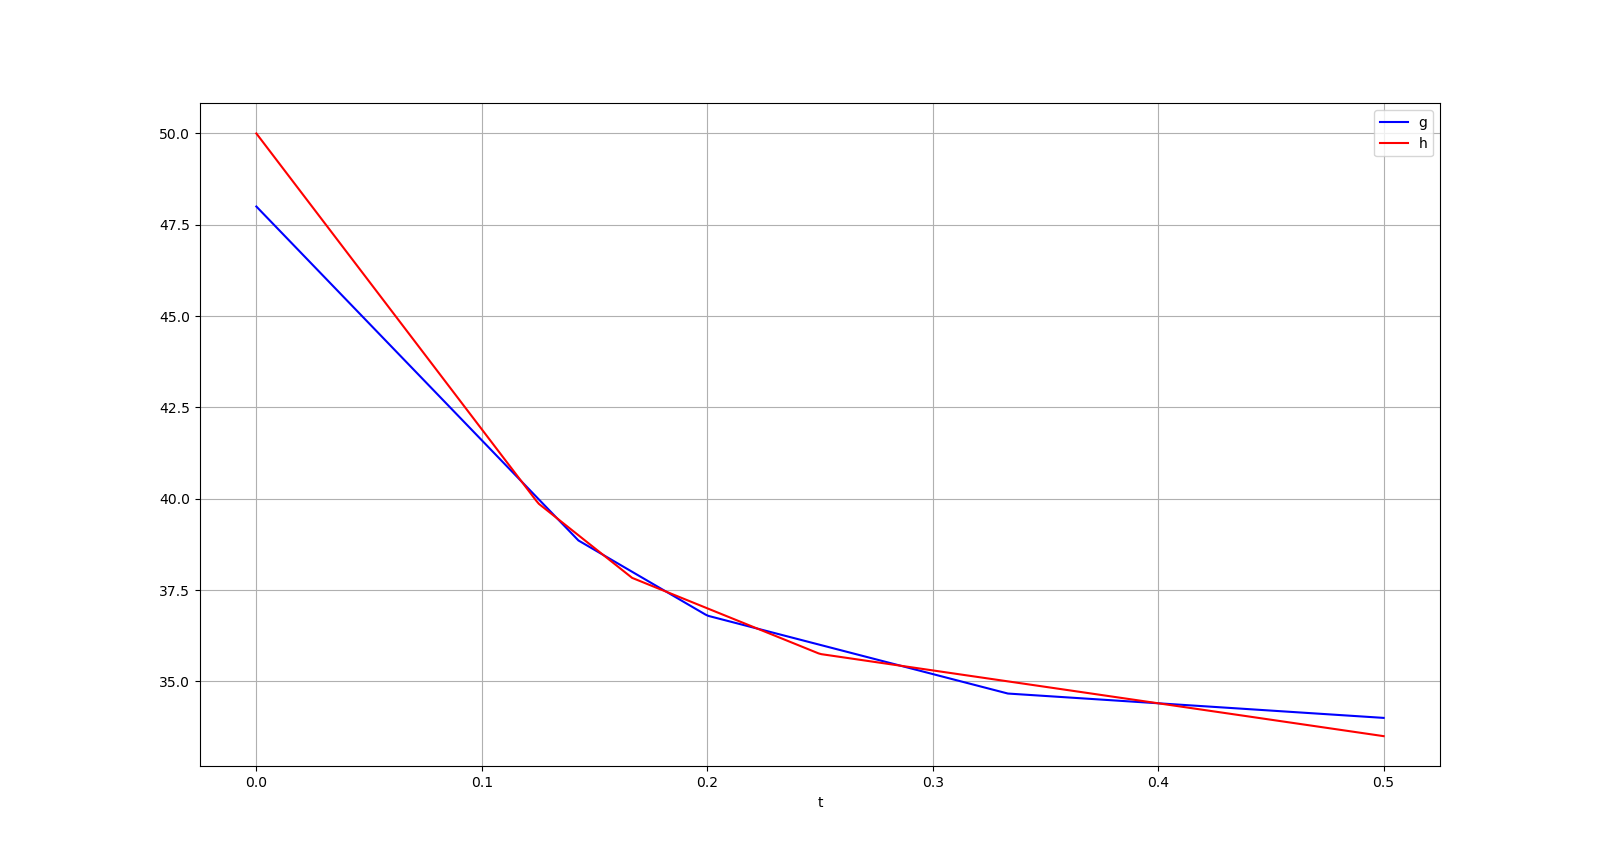
\includegraphics[scale=1, width=0.9\linewidth]{figures/chebyshev-eq-red.png}
		\caption{Example of the two functions constructed for the Chebyshev equation problem. Here the integer sequence \(1, 2, 3, 4\) was used. These functions do not change if any of the integers appear more than once. }
		\label{fig:chebyshev-eq-red}
	\end{figure}


	We define the function \(f_a(t) = C + 2a - a^2 t\) which corresponds to the maximized term on both sides without absolute value. The intuition behind this function is that \(f_a\) is the tangent on the function \(C + \frac{1}{x}\) at \(x = \frac{1}{a}\). Note that \(f_a(\frac{1}{a}) > f_b(\frac{1}{a})\) for all \(a \neq b \in \R_{> 0}\) as 
	\begin{alignat*}{3}
		& 0 &&< (b-a)^2 \\
		\iff & 0 &&> -\frac{1}{a}(b-a)^2 =  2b -\frac{b^2}{a} - a \\
		\iff & C + 2a - \frac{a^2}{a} &&> C + 2b -\frac{b^2}{a}.
	\end{alignat*}

	This means that the functions \(g(t) = \max_{i=1,\dots, d} f_{2x_i}(t)\) and \(h(t) = \max_{i=1,\dots, d} f_{2x_i+1}(t)\) consist of exactly \(d'\) many distinct line segments where \(d'\) is the amount of distinct elements as each corresponds to exactly one line segment. From \(t=0\) towards \(t = \frac{1}{2}\) all line segments are encountered in descending order of the respective \(x_i\) where the last line segment is encountered at least after \(t=1\) as we are dealing with integers and thus the maximal value of \(\frac{1}{n}\) is \(1\). 

	Note that these two functions are almost the ones from \cref{eq:red-eq-chebyshev} but without the absolute values. Thus, if all of their linear functions are positive on \([0,\frac{1}{2}]\) these two functions are equal to the sides of the equation. For \(C = \max_{i=1, \dots, d}2x_i^2\) it can be easily checked that all linear terms are positive on \([0, \frac{1}{2}]\).

	We now investigate the solutions to the equation \(g(t) = h(t)\) on \([0, \frac{1}{2}]\). For \(t = \frac{1}{2x_i}\) it holds \(g(t) > h(t)\) and for \(t = \frac{1}{2x_i + 1}\) it holds \(g(t) < h(t)\) for all \(i \in \set{1,\dots, d}\). Let \(d'\) again be the number of distinct elements. There are at least \(2d' - 1\) many solutions to the equation as there are \(2d'\) many distinct points of the form \(\frac{1}{2xi}\) and \(\frac{1}{2x_i+1}\) and the sign of \(g(t)-h(t)\) alternates between each of them. However, there cannot be more than \(2d'-1\) many solutions as each of the \(d'\) many line segments in \(g\) can only intersect at most \(2\) line segments in \(h\) because both are convex and the first and last line segment cannot both intersect \(h\) twice. Thus the amount of solutions in \([0,2]\) is exactly \(2d'-1\). 

	To decide the integer element distinctness, we construct \cref{eq:red-eq-chebyshev} and find the solutions. We iterate over them in linear time and count how many solutions there are in the interval \([0, \frac{1}{2}]\). This gives us \(2d'-1\) from which we can determine the amount of distinct elements.
\end{proof}

\begin{lemma}
	The Manhattan equation problem as stated in \cref{def:manhattan-problem} has a lower bound of \(\Omega(d \log d)\).
\end{lemma}

\begin{proof}
	Given an instance of the integer element distinctness problem \(x_1, \dots, x_d \in \N_+\). We construct the following instance of the Manhattan equation problem in \(2d\) dimensions. 
	\begin{equation}\label{eq:red-eq-manhattan}
		1 + \sum_{i=1}^d |6x_i + 4 - 2t| = \sum_{i=1}^d \parenth{|3x_i + 1 - t| + |3x_i + 3 - t|}
	\end{equation}
	
	For example instances see \cref{fig:manhattan-eq-red-1} and \cref{fig:manhattan-eq-red-2}. For a comparison of the subfunctions \(|6x_i + 4 - 2t|\) and \(|3x_i + 1 - t| + |3x_i + 3 - t|\) see \cref{fig:manhattan-building-block}.

	\begin{figure}
	  \centering
	  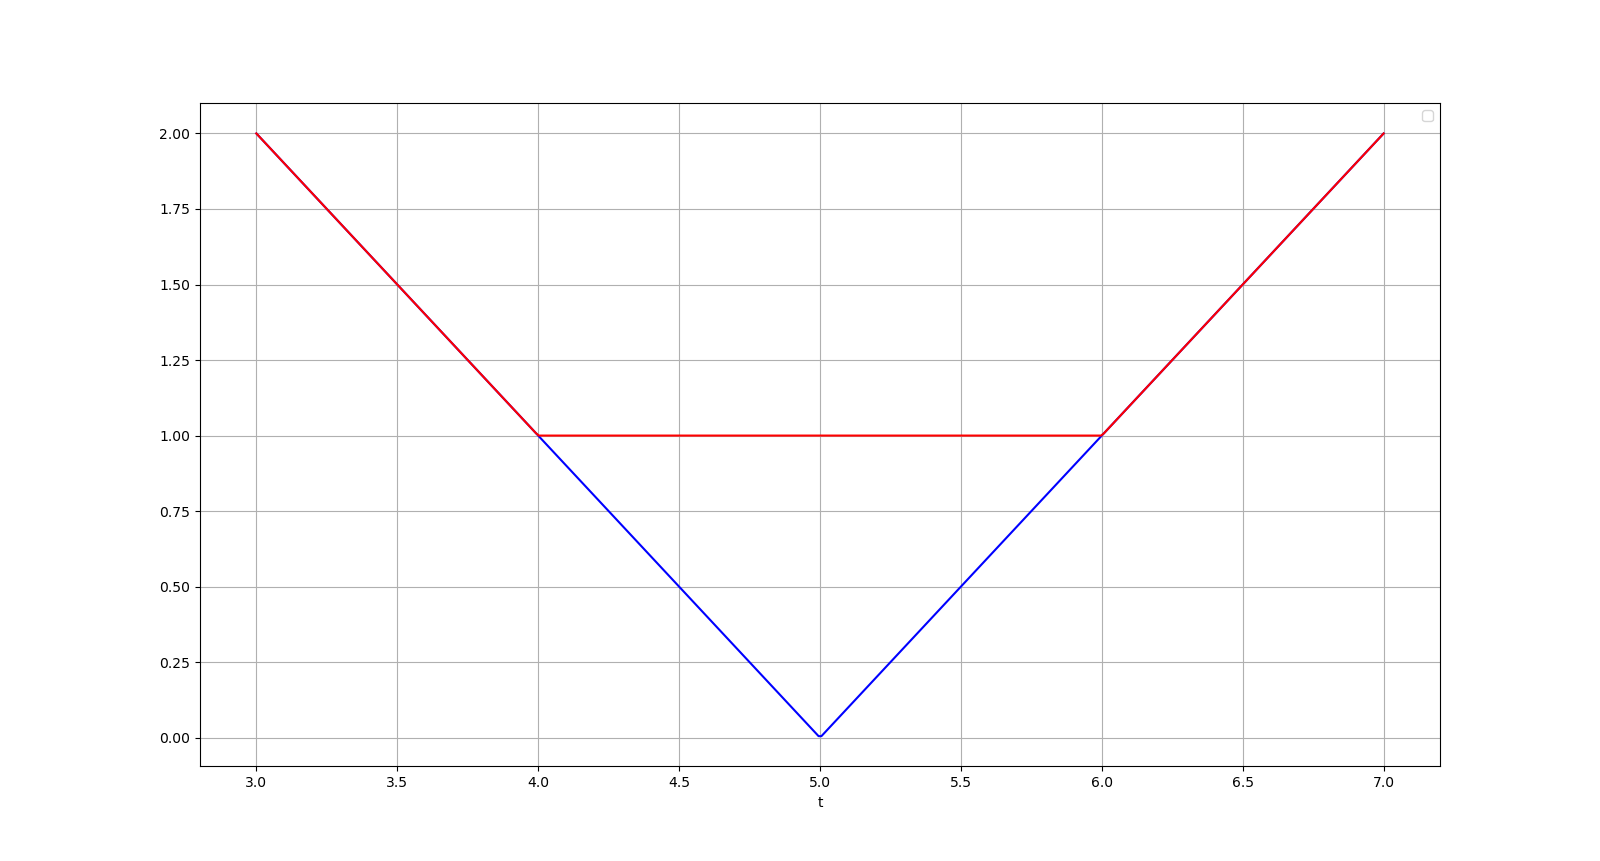
\includegraphics[scale=1, width=0.9\linewidth]{figures/manhattan-building-block.png}
	  \caption{Comparison of the functions \(|6x_i + 4 - 2t|\) and \(|3x_i + 1 - t| + |3x_i + 3 - t|\) for \(x_i = 1\).}
	  \label{fig:manhattan-building-block}
	\end{figure}

	\begin{figure}
	  \centering
	  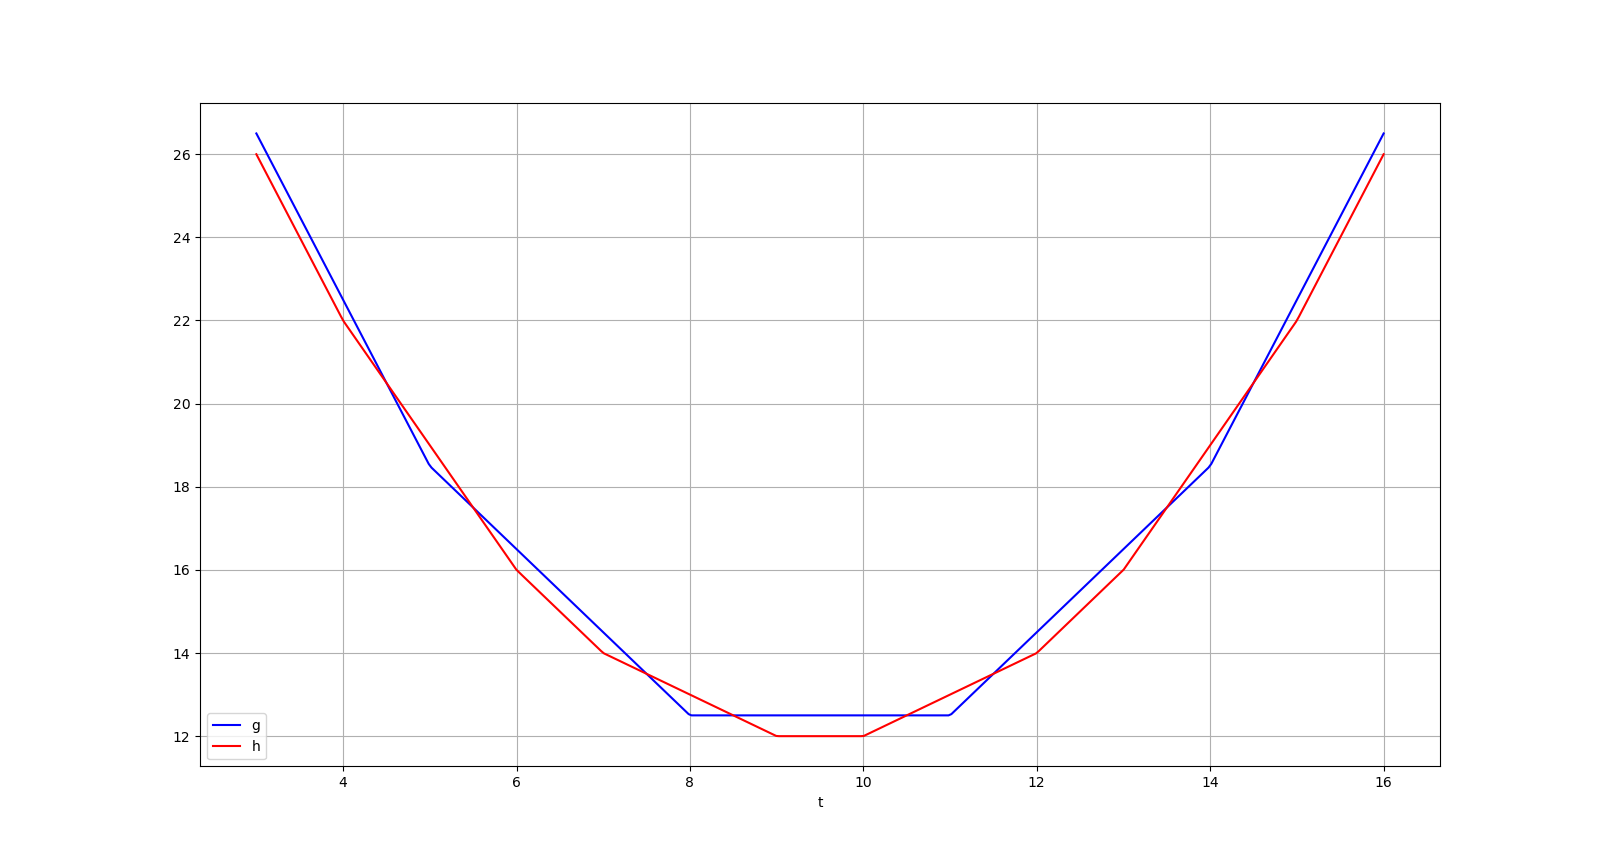
\includegraphics[scale=1, width=0.9\linewidth]{figures/manhattan-eq-red-1.png}
	  \caption{Instance for the numbers \(1,2,3,4\). There are \(8\) solutions which means there are \(4\) distinct values.}
	  \label{fig:manhattan-eq-red-1}
	\end{figure}

	\begin{figure}
	  \centering
	  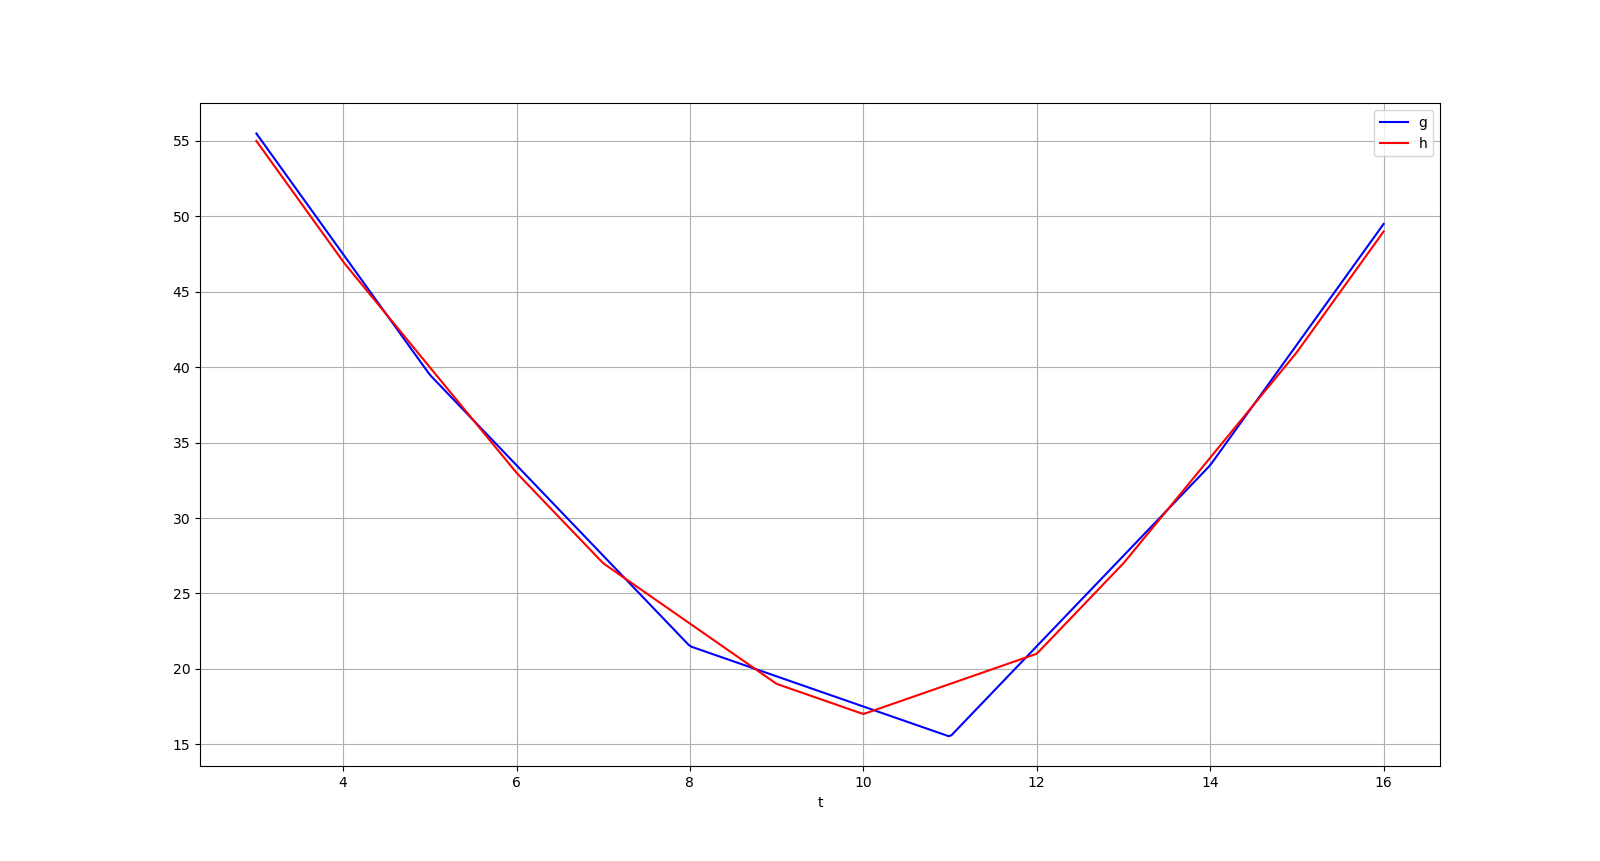
\includegraphics[scale=1, width=0.9\linewidth]{figures/manhattan-eq-red-2.png}
	  \caption{Instance for the numbers \(1,2,3,4,3,2,3,3\). The numbers \(2\) and \(3\) appear multiple times. This does not affect the amount of solutions but slightly moves their positions.}
	  \label{fig:manhattan-eq-red-2}
	\end{figure}

	It can easily be seen that for \(t \notin [3x_i + 1, 3x_i + 3]\) that \(|6x_i + 4 - 2t| = |3x_i + 1 - t| + |3x_i + 3 - t|\) and for \(t \in (3x_i + 1, 3x_i + 3)\) we get \(|6x_i + 4 - 2t| < |3x_i + 1 - t| + |3x_i + 3 - t|\). Further, the equation \(1 + k|6x_i + 4 - 2t| = k|3x_i + 1 - t| + k|3x_i + 3 - t|\) has exactly two solutions, both of which are in the interval \([3x_i+1,3x_i+3]\) for any \(k \in \N_+\). Set \(g(t) = 1 + \sum_{i=1}^d |6x_i + 4 - 2t|\) and \(h(t) = \sum_{i=1}^d \parenth{|3x_i + 1 - t| + |3x_i + 3 - t|}\).

	For \(t \in [3x_i, 3x_i + 1]\) for any \(x_i\) we can see that \(g(t) = 1 + h(t)\). For \(t \in (3x_i+1, 3x_i + 3)\) both sides of the equation are mostly the same, more specifically, \(g(t)- h(t) = 1 + k|6x_i + 4 - 2t| - k|3x_i + 1 - t| - k|3x_i + 3 - t|\) where \(k\) is the amount of datapoints which have the value \(x_i\). This has exactly two solutions in the interval. Thus the total amount of solutions is \(2d'\) where \(d'\) is the amount of distinct solutions.
\end{proof}





\section{Adapting Imai and Iri to the Global Fréchet Distance}
\label{sec:global_imai_iri}

In this section, we revisit the well-known \citeauthor{computational_geometric_methods_for_polygonal_approximations_of_a_curve}~\cite{computational_geometric_methods_for_polygonal_approximations_of_a_curve} algorithm for local Fréchet polyline simplification and demonstrate how to adapt it to the global Fréchet setting. By using different graph traversals, we can obtain the algorithm from \citeauthor{on_optimal_polyline_simplification_using_the_hausdorff_and_frechet_distance}, as well as rediscover a simplification algorithm from \citeauthor{global_curve_simplification}. We modify the algorithm slightly to create a simple cubic time heuristic which achieves optimality in many cases. This heuristic uses only quadratic space in the worst case, and for sufficiently well-behaved polylines, it can achieve a runtime of \(\Oh(n^2)\) and a space consumption of \(\O(n)\).

Throughout this section we fix \(\varepsilon > 0\) and a distance \(\delta\). Further, let \(P\) be a polyline of length \(n\). We note that some of the lemmas in this section can be seen rather trivial in the free space diagram. We have chosen not to use the free space diagram formalism in this thesis, as it introduces a layer of abstraction that we find obscure the intuitive mechanics of the algorithms presented. Furthermore, as it was not required for preceding sections, introducing it here would necessitate a significant digression. We find the direct proofs of the following lemmas to be more concise and equally rigorous.

\subsection{Local Case}

We recall the algorithm in the local setting to identify where modifications are needed to adapt it to the global setting. 

The algorithm consists of two main parts: first, a shortcut graph is constructed and then, a shortest path computation yields the simplification.

The shortcut graph is a directed acyclic graph whose vertices correspond to the polyline vertices. A directed edge \((P(i), P(j))\) with \(i < j\) exists if \(\delta^F(P[i \dots j], \overline{P(i)P(j)}) \leq \varepsilon\) (i.e., \(\overline{P(i)P(j)}\) is a shortcut for the subpolyline \(P[i \dots j]\)). 

To determine whether \(\delta^F(P[i \dots j], \overline{P(i)P(j)}) \leq \varepsilon\), we use the algorithm from \citeauthor{computing_the_frechet_distance_between_two_polygonal_curves}, modified versions of which are outlined in \cref{ssec:alt_godau,ssec:implicit_frechet_decision}. Here, the simpler classical version suffices. This test requires \(\Oh(n)\) time and as there are \(\O(n^2)\) many pairs to test, constructing the shortcut graph requires \(\Oh(n^3)\) time.

Each path from \(P(0)\) to \(P(n)\) corresponds to a valid, not necessarily optimal, local simplification of the polyline by construction and it is obvious that all such simplifications are captured in the shortcut graph. Thus, computing the shorted \(P(0)-P(n)\) path in this graph yields an optimal local simplification. This can be done easily in \(\O(n^2)\).

The total runtime is determined by the cubic graph construction phase thus the total runtime is \(\Oh(n^3)\).

\subsection{The Global Shortcut Graph}
In the global case the structure of these shortcuts is more complicated, necessitating a more sophisticated approach. To confront this problem, we store for each shortcut the set of all subpolylines for which it is a valid shortcut. 

\begin{definition}
  For a shortcut \(e = \overline{P(i')P(i)}\) we say that \((t', t) \in [0, n]^2\) with \(t' \leq t\) is \emph{\(e\)-admissible} if and only if \(\delta^F(P[t' \dots t], e) \leq \varepsilon\). We denote \(\mathcal{A}_e = \set{(t', t) \mid (t', t) \textrm{ is } e\textrm{-admissible}}\) as the set of \(e\)-admissible subpolylines.
\end{definition}

The following observation might seem complicated, but it follows directly from the definitions of admissibility and Fréchet distance. It captures our intuition that global simplifications are constructed of only admissible subpolylines.

\begin{observation}
	Let \(Q=\angl{P(u_0), \dots, P(u_q)}\) be a (not nessarily optimal) global simplification of \(P\) which means there are parameterizations increasing, continuous \(f, g\) with \(f([0, 1]) = [0, n]\) and \(g([0,1]) = [0, q]\) with \(\delta(P(f(\alpha)), Q(g(\alpha))) \leq \varepsilon\) for all \(\alpha \in [0, 1]\).

	Then, for \(i \in \set{1, \dots, q}\) and \(x \leq y \in [0, 1]\) such that \(g(x) = i - 1\) and \(g(y) = i\) it holds that 
	\[\delta^F(P[f(x) \dots f(y)], \overline{P(g(x)), P(g(y))}) \leq \varepsilon.\]
	This means \((f(x), f(y))\) is \(e\)-admissible for \(e = \overline{P(g(x), P(g(y)))} = \overline{Q(i-1), Q(i)}\).
\end{observation}

Next, we explore the set of admissible subpolylines \(\mathcal{A}_e\) with the goal of establishing an efficient representation.

\begin{lemma}\label{lem:admissible_are_intervals}
	Let \(e = \overline{P(i')P(i)}\).
  \begin{enumerate}
		\item Let \((r, t)\in \mathcal{A}_e\) and \(r \leq t' \leq t\) with \(\delta(P(t'), P(i')) \leq \varepsilon\). Then \((t', t) \in \mathcal{A}_e\).
		\item Let \((t', r)\in \mathcal{A}_e\) and \(t' \leq t \leq r\) with \(\delta(P(t), P(i)) \leq \varepsilon\). Then \((t', t) \in \mathcal{A}_e\).
  \end{enumerate}
\end{lemma}

\begin{proof}
	We show the first statement. The second one is analogous. We create suitable parameterizations \(f\) and \(g\) to show \(\delta^F(P[t' \dots t], e) \leq \varepsilon\). As \((r,t)\) is \(e\)-admissible, there are functions increasing, bijective parameterizations \(f':[0,1] \to [r \dots t]\) and \(g':[0,1] \to [0,1]\) (here we shift the range of \(f'\) to be consistent with \(P\) and not the subpolyline \(P[r \dots t]\)).

	Since \(f'\) is surjective onto \([r, t]\) and \(t' \in [r, t]\), there is \(x \in [0, 1]\) with \(f'(x) = t'\). This means that \(\delta(P(t'), e(g'(x))) \leq \varepsilon\). By the convexity property in \cref{lem:distance_properties}, \(\delta(P(t'), e(\lambda)) \leq \varepsilon\) for all \(\lambda \in [0, g'(x)]\). With this, we construct the parameterizations \(f\) and \(g\) such that \(f\) is the zero function until \(g\) assumes the value \(g'(x)\). After this point both functions are identical to \(f'\) and \(g'\) respectively (up to a shift in the range).
\end{proof}

\begin{definition}
	For sets \(A\) and \(B\) we define \(A \times_{\leq} B\) to be 
		\[A \times_{\leq} B = \set{(a, b) \in A \times B \mid a \leq b}.\]
\end{definition}

Using \cref{lem:admissible_are_intervals}, we define an efficient representation of \(\mathcal{A}_e\).
\begin{lemma}\label{lem:admissible-rep-1}
	Let \(e = \overline{P(i')P(i)}\) be a line segment. Denote \(\mathcal{I} = \set{t \in [0,n] \mid \delta(P(i'), P(t)) \leq \varepsilon}\) and \(\mathcal{J} = \set{t \in [0,n] \mid \delta(P(i), P(t)) \leq \varepsilon}\). There exist \(k \leq n\) and families of closed intervals \(I_1 \leq \cdots \leq I_k\) and closed intervals \(J_1 \leq \cdots \leq J_k\) such that 
	\[\mathcal{A}_e = \parenth{\mathcal{I} \times_\leq \mathcal{J}} \cap \bigcup_{j=1}^k I_j \times J_j.\]

	Here, the ordering on the intervals is defined by their lower bounds or equivalently by their upper bounds. It is further possible to achieve that the family \(I_j\) is pairwise disjoint or that the family \(J_j\) is pairwise disjoint (but not necessarily both).
\end{lemma}

\begin{proof}
	The lemma is trivial if \(\mathcal{A}_e\) is empty. Suppose it is not empty. It holds by definition that \(\mathcal{A}_e \subseteq \mathcal{I} \times_\leq \mathcal{J}\). 

	For any \(e\)-admissible subypolyine \((t', t)\) there exist closed maximal intervals \(I\) and \(J\) with \(t' \in I\), \(t' \in J\), and \(I \subseteq \mathcal{I}\) and \(J \subseteq \mathcal{J}\) by the distance constraints on the endpoints by the definition of the Fréchet distance. 

	We show that \(I \times_\leq J \subseteq \mathcal{A}_e\): pick any \(s' \leq s\) with \(s' \in I\) and \(s \in J\). If \(s' \leq t'\) then \(\delta^F(P[s' \dots t'], P[y \dots y]) \leq \varepsilon\) for any \(y \in J\) by construction of \(I\) and \(J\), and thus, we can extend any admissible \(t', y\) subpolyline to an admissible \((s', y)\). Similarly, if \(s \geq t\), for any \(x \in I\), we can extend admissible \((x, t)\) subpolylines to admissible \((x, s)\) subpolylines. Therefore, we can assume \(s' \geq t'\) and \(t \leq s\). Under these conditions, it follows that \((s', s)\) is admissible by using \cref{lem:admissible_are_intervals}.

	We now have seen that admissibility is a property shared by pairs of intervals, not only points. Thus, we will say \((I, J)\) is admissible if all point pairs \((t', t)\) with \(t' \leq t\) in \(I \times J\) are admissible.


	This shows that \(\mathcal{A}_e\) has almost such a structure. We need to show that \(k \leq n\) many interval pairs suffice. For this, we merge intervals: Let \(I < I'\) disjoint and \(J\) be closed intervals that we have already selected for the construction. Furthermore, assume that \((I, J)\) and \((I', J)\) are admissible. By \cref{lem:admissible_are_intervals}, for any point \(x \in [\min I, \max I'] \cap \mathcal{I}\) any \(y \in J\) with \(x \leq y\) must form an admissibily subpolyline \((x, y)\). Thus we merge all such intervals \(I'\) and \(I\) to form an interval of intervals per interval \(J\). This does not introduce no inadmissible subpolylines, as we already filter by \(\mathcal{I} \times_\leq \mathcal{J}\). As each interval \(J\) has a unique range of intervals \(I\), the \(J_j\) are disjoint. By merging the \(J\) per \(I\) instead, we can achieve disjointness of \(I_j\).

	The total number of interval pairs is bounded by the number of possible closed intervals that make up \(\mathcal{I}\) and \(\mathcal{J}\). There can be at most one closed interval per line segment of the polyline, thus \(k \leq n\), concluding the proof.
\end{proof}


\begin{definition}[Global Shortcut Graph]
	For a polyline \(P = \angl{v_0, \dots, v_n}\) and \(\varepsilon > 0\) we define the global shortcut graph as the directed acyclic graph \(G = (V, E)\) with \(V = \set{v_0, \dots, v_n}\) and \(E = \set{(v_i, v_j) \mid i < j, e = \overline{v_iv_j}, \mathcal{A}_e \neq \emptyset}\).

	We define a labelling function on the edges that assigns to each edge \(e\) the list of interval pairs from its admissible set representation:
	\[S(e) = ((I_1, J_1), (I_2, J_2), \dots, (I_k, J_k)),\]
	where the families of intervals \(\set{(I_i, J_i)}_{j=1}^k\) are constructed in the proof of \cref{lem:admissible-rep-1}. We extend this labelling on the vertices by \(S(v) = (I_1 < \cdots < I_k)\), which are the intervals that make up \(\mathcal{I}\) from the lemma.

	We refer to intervals \(I \in S(v)\) as \emph{solution intervals} as they are defined by solving equations. A pair \((I, J) \in S(e)\) will be referred to as a \emph{(interval) mapping} as the describe how to map points \(I\) to points in \(J\) using the shortcut \(e\).
\end{definition}

Let us briefly analyze the space consumption of the global shortcut graph: for each line segment, we may need to store up to \(n\) mappings, which in total requires cubic space. There are at most \(n\) solution intervals in \(\mathcal{I}\) per point, thus requiring total quadratic space. The total information of the global shortcut graph requires \(\O(n^3)\) space in the worst case. However, this is a pessimistic bound since solution intervals can span multiple line segments which we merge into a single interval to obtain fewer intervals. For further analysis, we denote \(\mathcal{E}\) the total number of mappings in the edges and \(\mathcal{V}\) for the number of solution intervals for the vertices. The total space thus is \(\O(n^2 + \mathcal{E})\).

We finally consider the runtime of constructing the global shortcut graph. For the point \(u\), the solution intervals \(S(u)\) can be determined by solving the necessary equation for each line segment of \(P\) and potentially merging ones that span multiple line segments. This takes runtime \(\Oh(n)\) per point and thus in total \(\Oh(n^2)\). 

To determine the mappings in \(S(e)\) for the line segment \(e = \overline{P(i')P(i)}\), we use a modified version of \citeauthor{polyline_simplification_has_cubic_complexity_bringmannetal}'s cell reachability algorithm that we have outlined in \cref{ssec:cell_reachability}.

\subsection{Modified Cell Reachability}
We describe how to modify the cell reachability problem to construct the interval mappings in \(S(e)\). We are given the ordered lists of solution intervals \(S(i')\) and \(S(i)\) and want to find the mappings between them. 

The setting is rather similar to \cref{ssec:cell_reachability} with few differences. First, there are no entry- or exit-costs, we only track admissibility. Second, the result is an interval \(J_j\) for each admissible interval \(I_j\). The passages between cells are the solution intervals of \(e\) and the respective vertex. For an example instance refer to \cref{fig:ex_cr_globalii}.

The core algorithm from \cref{ssec:cell_reachability} requires only minor modifications to compute the interval mappings \(S(e)\). The key changes are in how the queue of reachable cells is maintained when encountering a solution interval. Specifically, for each passage, we remove all queue entries at the front with a value below the lower lower bound of the passage and reinsert them as a single entry whose value is the lower bound. Each entry is now associated with an interval of indices which correspond to the intervals in \(S(i')\). When merging, we update the upper bound of the indices interval. If an interval in \(S(i')\) starts before the cell passage, it must be accounted for during the merging step.

Then, we remove all entries that lie above the upper end of the passage. Each of them contains an indices interval that represent  the intervals for which the last seen \(S(j')\) interval is the upper end. For all of these intervals we update their upper bound.

The intervals in \(S(i)\) can be ignored, if we are only interested to compute maximal intervals \(J_j\) for each \(I_j\). We can consider them to only store discrete intervals that represent the intervals in \(S(i)\) that are to be used.

\begin{figure}[htb]
  \centering
  \includegraphics[scale=1, width=0.9\linewidth]{./tikz-fig/ex_cr_globalii.pdf}
	\caption{Cell reachability example for computing \(S(\overline{P(0)P(1)})\). Here, \(S(0) = ([0, 0.5], [2.5, 2.5]), [3.59, 4.36]\) are marked in blue, and \(S(1) = ([0.5, 1.70], [2.5, 2.5], [4.64, 5])\) are marked in red. The one point interval \([2.5,2.5]\) is shared by both and is marked in purple. It is not a vertex of the polyline. We can see that \(S(\overline{P(0)P(1)}) = (([0,0.5], [0.5,5]), ([2.5,2.5],[2.5,5]), ([3.59,4.36],[4.64,5]))\).}
  \label{fig:ex_cr_globalii}
\end{figure}

A small optimization that can be applied is to skip cells when the queue becomes empty and resume at the next \(S(i')\) interval. Using this, the total runtime per line shortcut is proportional to the total length of the intervals which extends to the construction of the shortcut graph. Furthermore, we can actually skip all computations when adding an interval up to the end of the interval if it is the only element in the queue (and thus especially for the first interval). This is because the lower bound for the interval is zero throughout the interval.

\subsection{Simplification Construction}\label{ssec:simplification_construction}

To construct the simplifications from the graph, we iterate through it using the admissible subpolylines. Any simplification is a sequence of \(e_i\)-admissible subpolylines where the sequence of edges \(e_i\) form a 0-n-path and the endpoints of two consecutive subpolylines match.

Unlike the local case, it does not suffice to find a shortest path, thus we have to consider more wisely how to iterate through the graph. Interestingly, we can derive the algorithm from \citeauthor{on_optimal_polyline_simplification_using_the_hausdorff_and_frechet_distance} using suitable graph traversels: we start with \(S(0)\) as the starting interval and traverse the graph. In the subsequent traversals we repeat this procedure but start with the computed intervals from the last step. We stop once an interval is found that contains the endpoint of the polyline.

From this, we can see why the \citeauthor{on_optimal_polyline_simplification_using_the_hausdorff_and_frechet_distance} algorithm has poor runtime: we iterate through the whole graph multiple times. Furthermore, their algorithm does not precompute the global shortcut graph but computes everything once it is used which also means that the same computations are performed multiple times. Using our precomputed graph the runtime can be reanalyzed as follows: let the simplification size be \(k\), then the total runtime is \(\Oh(n^3 + kf(n))\) where \(f(n)\) is the runtime per iteration and \(\Oh(n^3)\) the runtime to construct the graph.

Let us analyze how many intervals there can be at most that need to be tracked: each interval is paired with an vertex from the polyline where the vertex represents the last point of the partial simplification (i.e., the point form which we start the next shortcut) and the interval is the end of the subpolyline. As seen previous, there can be at most one interval per line segment but as it can be paired with different points, there can be in total \(\O(n^2)\) many intervals per iteration to track. For each interval we must iterate over all possible shortcuts that start from its associated end vertex to compute the next interval and verex pairs. There are at most \(\O(n^2)\) many possibilities to iterate through, resulting in \(\O(n^4)\) runtime per traversal and thus in total \(\Oh(kn^4)\) runtime. This improves upon the standard algorithm by \(\O(n)\). Furthermore, this version of the algorithm benefits more from the well-behavedness of the input by having fewer intervals to track.

To obtain a better runtime, we traverse the graph only once. The most obvious iteration order is through the graph vertices which corresponds to the same order in the algorithm by \citeauthor{polyline_simplification_has_cubic_complexity_bringmannetal} however the resulting algorithm is different. We track all subpolylines that have a partial simplification that end in the currently tracked vertex. In the local case we iterate for each vertex over all previous vertices, test if there is a shortcut to the current vertex and if so extend the partial simplification and use the minimal found partial simplification. In the global case, we can also minimize over all previously computed values and extend the previously found partial simplifcations to one ending in the current vertex, however there is more data to track.

First, we consider how much data needs to be tracked per vertex in the iterations. Each subpolyline is an interval on the polyline. Per line segment on the polyline at most \(n\) many subpolylines can start because we track only minimal subpolylines. Each subpolyline is associated with the length of the partial simplification up to this point so if we have two subpolylines starting on the same line segment with the same length, we only need to track the one with the earlier start. Thus in total only \(\O(n^2)\) subpolylines can exist.

To propagate these subpolylines for the vertex \(i\), we iterate over all \(j < i\) and use \(S(\overline{P(j)P(i)})\). We iterate over all values in \(S(j)\) to find the previous subpolylines and iterate over all mappings in \(S(\overline{P(j)P(i)})\). We iterate in simultaneously over both of them to determine all possible subpolylines that use \(j\). As \(S(j)\) has \(\O(n^2)\) many subpolylines, the mapping also requires \(\O(n^2)\) time. As this needs to be done for all \(j < i\) we get cubic runtime for the mapping. We finally need to merge all the computed subpolylines which can be done while mapping by using \(n\) linked lists, one for each line segment. Each of those lists has size \(\O(n)\) and we can store pointers to the list elements in an array to find in constant time the position of a subpolyline with a given simplification size. For this, we observe the on each line segment, the subpolylines are ordered by the start of the subpolyline in ascending order and the size of of the simplification in descending order (if a subpolyline start before another one and requires a shorter simplification, the other one can be removed).

This results in a \(\Oh(n^4)\) algorithm, as we perform \(\O(n)\) propagation steps (one per vertex), each of which involves \(\O(n)\) predecessors, and for each predecessor, \(\O(n^2)\) work for processing intervals and mappings, yielding \(\O(n^3)\) work per step. Using insights from \citeauthor{polyline_simplification_has_cubic_complexity_bringmannetal}, \citeauthor{global_curve_simplification} further improved the runtime to \(\Oh(n^3)\). Both algorithms works essentially the same way but with a different order of computation.

\subsection{Cubic Runtime Heuristic}
As the cubic runtime variant of this algorithm is very similar to the \citeauthor{polyline_simplification_has_cubic_complexity_bringmannetal} algorith, we instead establish a simpler heuristic which results in smaller simplifications than local simplifications and achieves optimal results in many cases.

The main problems of the cubic variants are their rigid structure that force a cubic number of computations which seem to be resistant to further optimizations. The current \(\Oh(n^4)\) algorithm can adapt to the input to achieve up to near quadratic runtime and space in the best case.

To achieve worst case \(\Oh(n^3)\) time and quadratic space with possibly quadratic runtime for well-behaved polylines, we introduce a new heuristic based on the case distinction that both of the cubic runtime algorithms make. In \citeauthor{polyline_simplification_has_cubic_complexity_bringmannetal}'s algorithm, we distinguish the case carrying over the earliest reachable point on the same line segment or setting the earliest reachable point to the start of the solution interval when comparing different line segments. The first case is computed using a simple minimum computation while the second one requires the cell reachability procedure.

Even though the first of the two cases is simpler to compute, it causes the most problems: It is the reason why we need cubic space as we need to track linearly many points per line segment and vertex; the second case only requires one datum per line segment. Additionally, intuitively this case is less likely to affect the simplification. In this case we have multiple consective shortcuts that make little progress on the polyline which is in opposition to the goal of achieving as few shortcuts as possible. Furthermore, interval mappings that allow make this case necessary have a restrictive nature. 

To formlize our approach, we split mappings into three categories:
\begin{definition}
	Let \(m = ([a, b], [c, d])\) be a mapping in the global shortcut graph. We call \(m\)
	\begin{itemize}
		\item \emph{positive} if \(b \leq c\),
		\item \emph{neutral} if \(a \leq c \leq b\),
		\item \emph{negative} if \(c < a\).
	\end{itemize}

	We call global shortcut graph positive if it has no negative mappings. A polyline is called \(\varepsilon\)-positive its global shortcut graph is positive. If \(\varepsilon\) is clear from context we will omit it.
\end{definition}

\begin{theorem}
	Let \(\varepsilon > 0\) and \(P\) be positive polyline. Then \(\delta^F(P, \varepsilon)\) can be computed in \(\Oh(n^3)\) with quadratic space.
\end{theorem}

\begin{proof}
	In a positive polyline, for given vertices \(u\) and interval \(I \in S(u)\), the structure of the admissible mappings ensures that there is a unique 'best' (i.e., earliest starting point which is the start of the interval) subpolyline that achieves a partial simplification ending at \(u\) and covering \(I\). Therefore, an array of size \(\O(\mathcal{V}) \subseteq \O(n^2)\) suffices where we store for each vertex \(u\) and interval \(I \in S(u)\) the shortest partial simplification ending in \(u\) that reaches \(I\). For this only the preceding vertex and the size of the partial simplification need to be stored. With this, a graph traversal more similar to the algorithm from \citeauthor{computational_geometric_methods_for_polygonal_approximations_of_a_curve} can be applied. For each vertex \(v\), we iterate over all \(u < v\) and the reachable subpolylines in all reachable \(S(v)\) and their mappings \(S(\overline{uv})\). As all of these list are ordered and at most one mapping is applicable to any interval in \(S(v)\), the propagation onto \(u\) takes constant time per interval. For each vertex there are at most linearly many mappings and intervals to consider so by using the order, a merge-like procedure requires only linear time per \(v\) and thus quadratic time per \(u\). In total cubic runtime is achieved. 

	To reduce space to quadratic, we observe that we do not need to precompute the mappings as the mappings in \(S(\overline{uv})\) are used all at once when propagating reachability from \(u\) to \(v\) and thus, we can defer the computation to the propagation instead of storing them global. At any time only at most linearly many mappings are stored.
\end{proof}

As not every polyline is positive for a given \(\varepsilon\), we introduce a new heuristic simplification by transforming the global shortcut graph of the polyline into an positive one. This does not always yield optimal simplifications but the simplifications are never worse than local ones.

The first step is to split the unique interval \(I = [a, b] \in S(u)\) with \(u \in I\) into two intervals \([a, u]\) and \([u, b]\). The second and final step consists of narrowing the intervals in \(S(u)\) for all \(u\) and removing mappings in the following way. For any mapping negative \(([a,b], [c,d]) \in S(\overline{uv})\) with we either 
\begin{enumerate}
	\item update the first interval \([c, x] \in S(u)\) to \([a, x]\) if \(a \leq x\),
	\item If \(a > x\), we remove the interval \([c, x]\) from the mapping. If there are further intervals in the range of the mapping we repeat this process with the next interval until the first case occurs or no intervals remain in the range. In the latter case, we remove the mapping completely.
\end{enumerate}

After this process, the global shortcut graph is positive as we have modifed or removed all negative mappings. We now show that using this modified shortcut graph always yields a solution that is not worse than a local simplification. For this it suffices to show that all local shortcuts are still included. Take a local shortcut \(\overline{uv}\), which means that \(\delta^F(P[u \dots v], \overline{uv}) \leq \varepsilon)\). This means that \((u, v)\) is \(\overline{uv}\)-admissible and thus there is a mapping \((I, J) \in S(\overline{uv})\) with \(u \in I\) and \(v \in J\). Since we have split the solution intervals containing \(u\) in \(S(u)\), no intervals are removed in the process, and the intervals are only shrunk from the left, there is still an interval \([a, u]\) in \(S(u)\) and similarly for \(v\). The mapping that contains the local shortcut can not be removed by this process because \(u < v\). Thus all local shortcuts are still contained in the graph. Of course, a consequence of this is that this process can never remove too many mappings and thus will always find a solution.

To achieve quadratic space, we still do not need to precompute the whole global shortcut graph. When computing the reachable subpolylines for \(v\) the mappings in \(S(\overline{uv})\) only affect the solution intervals in \(S(v)\). It suffices to shrink the intervals as the mappings are computed and store the reachable subpolylines as an interval of indices (because the indices of the solution intervals do not change unlike their left bounds).

This heuristic can also be made into a simple optimal algorithm: for each negative mapping \(([a,b], [c,d]) \in S(\overline{P(i')P(i)})\) we split the interval \([c, d] \in (S(i))\) into two intervals \([c, a]\) and \([a, d]\). This basically transforms the heuristic back into the \(\Oh(n^4)\) algorithm as the amount of intervals can be quadratic per vertex. Using other interval-splitting and mapping-update strategies might yield better results than the outlined heuristic at the potential cost of runtime.

\subsection{Analysis of the Heuristic}
We have shown that our heuristic is never worse than a local simplification. Now, we analyze polylines on which the heuristic performs well and ones where it performes poorly.

The examples \cref{fig:local-global-bigdiff,fig:local-global-mostdiff} which have a high difference between the local and global simplifications can be solved optimally using our heuristic as both polylines are \(\varepsilon\)-positive using the given \(\varepsilon\). For further investigations into optimality criteria for the heuristic we differentiate polylines into two categories.

\begin{definition}
  Let \(P\) be a polyline and \(\varepsilon > 0\). We call \(P\)
	\begin{itemize}
		\item \(\varepsilon\)-\emph{neutral} if the result from the heuristic is optimal and 
		\item \(\varepsilon\)-\emph{negative} if the result from the heuristic is non-optimal.
	\end{itemize}
\end{definition}

Naturally, every positive polyline is also neutral and any the shortcut graph of a negative polyline contains at least one negative mapping. 

Let us present a few simple criteria for neutral polyines.
\begin{lemma}
  Let \(P\) be a polyline, \(\varepsilon > 0\) and \(G\) be the global shortcut graph of \(P\) using \(\varepsilon\). \(P\) is \(\varepsilon\)-neutral if any of these following conditions hold.
	\begin{enumerate}
		\item \(P\) is \(\varepsilon\)-positive.
		\item The local and global simplifications of \(P\) coincide.
		\item \(\varepsilon\) is at least as large as the distance between any pair of vertices of \(P\).
		\item \(S(i)\) contains exactly one solution interval and this unique interval contains only one polyline vertex (which must be \(i\)).
		\item \(\max \set{a \mid [a, b] \in S(i')} \leq \min \set{a \mid [a, b] \in S(i)}\) for all \(i' < i\).
	\end{enumerate}
\end{lemma}

\begin{proof}
	\begin{enumerate}
	  \item Already shown previously.
		\item The heuristic can never be smaller as the global simplification but it also cannot be larger than a local simplification.
		\item This implies both previous criteria. Each vertex contains exactly one interval \([0, n]\), i.e., each interval spans the whole polyline. As all intervals are the same there can be no negative mappings. Furthermore, this also implies that both the loval and global simplification only contain the start and end vertex.
		\item The interval in \(S(i)\) starts either on the line segment before the vertex \(i\) or the exactly on the vertex \(i\) (e.g., for \(i=0\)). Mapping the starts of the intervals onto the real numbers yields a monotone sequence. As shortcuts can only proceed to higher indexed vertices, the range interval must start after the domain interval and is thus neutral or positive. Thus, the polyline is positive.
		\item Follows directly from the proof for the last criterion.
	\end{enumerate}
\end{proof}

We present a negative polyline in \cref{fig:gii_diff_2}. The global simplification requires only four points while the heuristic needs 6. In the sequence of mappings in the global simplification there are no negative mappings, however, the heuristic stil cannot find it as the interval for the second vertex of the simplfication is shrunk because of other negative mappings. 

\begin{figure}[htb]
  \centering
  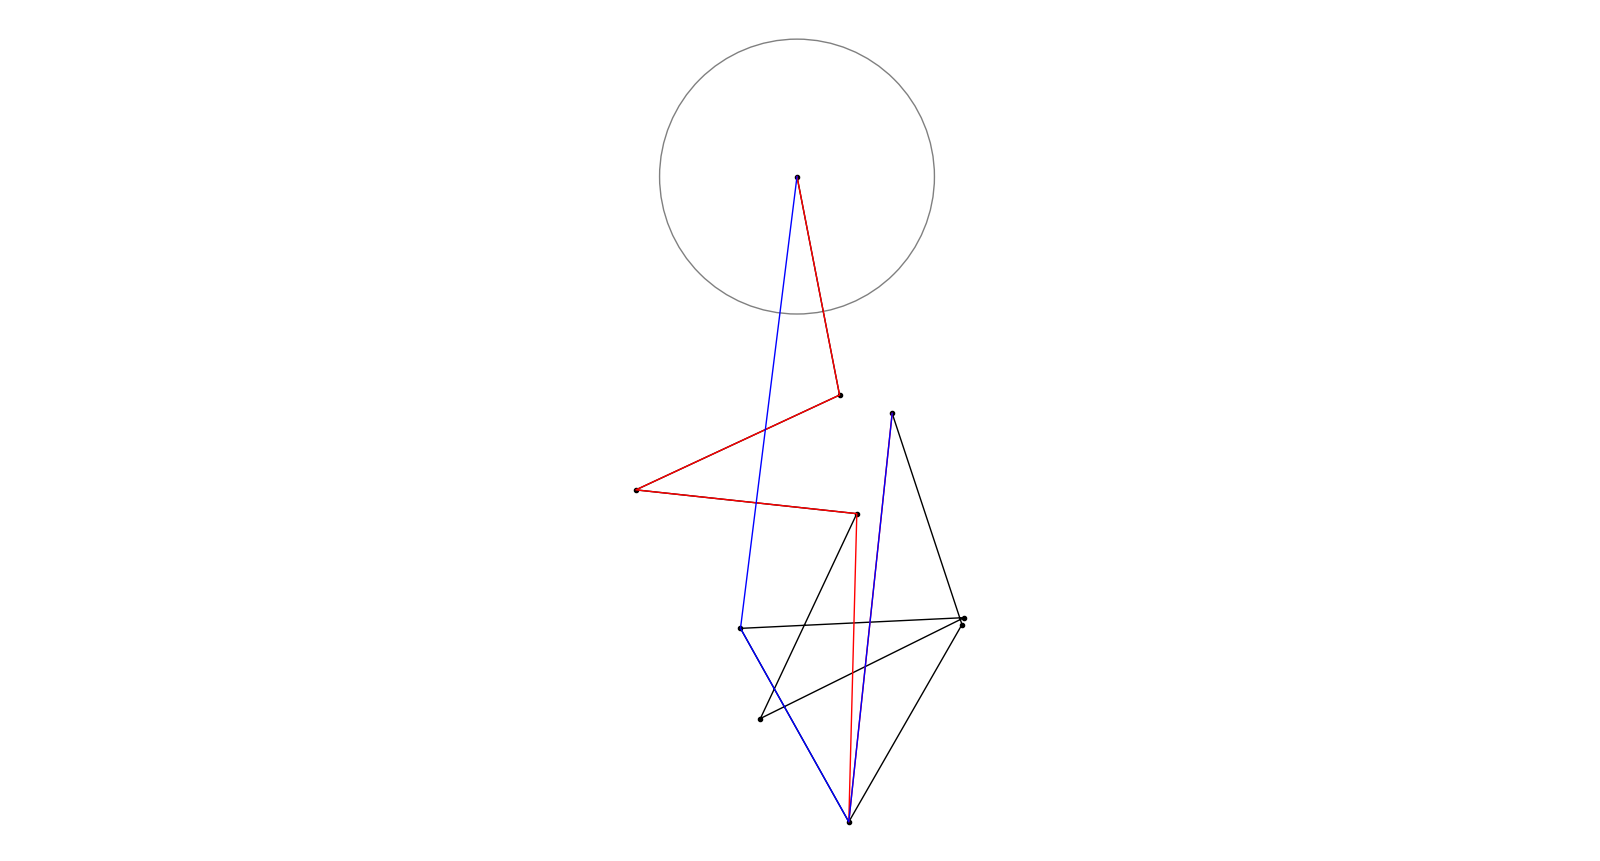
\includegraphics[scale=1, width=0.9\linewidth]{./figures/gii_diff_2.png}
	\caption{A negative polyline with 10 points. The difference between the heuristic and global simplification is 2. The last blue line segment is shared by both simplifications. The circle around \(P(0)\) has radius \(\varepsilon\).}
  \label{fig:gii_diff_2}
\end{figure}

We want to mention that we were not able to construct such an example ourselves. This example was found during testing on random polylines. We extracted the part that caused the difference into this example. Actually constructing polylines where the simplifications differ is non-trivial as negative mappings mostly arise in unintuitive substructures and to obtain a polyline with differing simplifications it is better to have multiple negative mappings.

\subsection{Conclusion}

This algorithm scheme generalizes \citeauthor{global_curve_simplification}'s algorithm and the \citeauthor{on_optimal_polyline_simplification_using_the_hausdorff_and_frechet_distance} algorithm but also the \citeauthor{computational_geometric_methods_for_polygonal_approximations_of_a_curve} algorithm. However, this approach is more complex than local simplification algorithms, and slower.

We have not shown any guarantees on our heuristic but it can easily be shown that is optimal on \cref{fig:local-global-bigdiff,fig:local-global-mostdiff} since those polylines are \(\varepsilon\)-proceeding. Thus, our heuristic is reasonable on some polylines where local simplifications suffer massively.

In their comprehensive study on global types of simplification, \citeauthor{global_curve_simplification} state ``what makes the problem difficult it is not well understood". We think our adaptation of the \citeauthor{computational_geometric_methods_for_polygonal_approximations_of_a_curve} algorithm to the global setting and the resulting heuristic make a convincing point that negative mappings and the resulting need to mainting large structures is a major difficulty.

We conclude with further research questions regarding the global shortcut graph and our heuristic.

\begin{itemize}
	\item	How much can the heuristic differ from the optimum?

	We gave an example where the heuristic's size was 6, while the optimal global simplification had size 4, a difference of 2 on a polyline of length 10. By replicating it with enough distance (similarly to \cref{fig:local-global-bigdiff}) we can create polylines with an arbitrary difference. However, this process can only create polylines where the difference is within a factor of \(1.5\). We do not know if the heuristic can be arbitrarily bad (like local simplifications) or whether an approximation guarantee can be established. We think that it can be arbitrarily bad by creating polylines with many negative mappings which reduce the intervals and thus disqualify many mappings which could be used for a global simplification but we have no construction to back this hypothesis.

	\item Which are strategies are there for the intervals and mappings?

	Our strategy is simple but comes with no guarantees as far as we know. More sophisticated update rules may allow for better simplifications while preserving the cubic time worst case and quadratic worst case space consumption.

	\item Under which conditions is a polyline positive or neutral?

	We have given some basic properties. However, our conditions are either trivial or are only useful as a certificate that the found heuristic is optimal. They are rather abstract which makes it hard to reason whether they are likely to apply to any class of polylines.

	\item Can the heuristic be implemented in (near-)quadratic runtime?

	For sufficiently nice polylines, the algorithm can achieve quadratic runtime. For this, there should be only few mappings and intervals, and the cell reachability to compute the mappings should use early exits as often as possible. 

	Our heuristic is structurally closer to the algorithm by \citeauthor{computational_geometric_methods_for_polygonal_approximations_of_a_curve} which has already been optimized to achieve that runtime (e.g. \cite{polyline_simplification_under_the_local_frechet_distance_has_almost_quadratic_runtime_in_2d_storandtetal}). It is still more complex than the local case as we do not only track one vertex but a list of intervals for each vertex. Some concept can be adapted, for example, \citeauthor{polyline_simplification_under_the_local_frechet_distance_has_almost_quadratic_runtime_in_2d_storandtetal} use wedges based on the unit circle around points to narrow down shortcuts. These can be adapted into the global setting by widening the wedges to all points on the respective subpolylines. 
\end{itemize}










% \section{Experimental Evaluation}
% \label{sec:evaluation}
% 
% \subsection{Experimental Setup}
% \label{subsec:exp_setup}
% 
% \subsection{Data and Hardware}
% \label{subsec:hardware}
% 
% \subsubsection{Software and Data}
% \label{subsubsec:software}
% 
% \subsubsection{Hardware}
% \label{subsubsec:hardware}
% 
% \subsection{Results}
% \label{subsec:results}
% 
% \section{Conclusions and Future Work}
% \label{sec:discussion_conclusion}

